%\documentclass[sigconf]{acmart}
\documentclass{style/vldb}


% Specific for acmart (CIKM) package
%\settopmatter{printacmref=false} % Removes citation information below abstract
%\renewcommand\footnotetextcopyrightpermission[1]{} % removes footnote with conference information in first column
%\pagestyle{plain} % removes running headers
%\usepackage{booktabs} % For formal tables, 


\usepackage{algorithm}
\usepackage{algorithmic}
\usepackage{color}
\usepackage{graphicx}
\usepackage{array}
\usepackage{caption}
\usepackage{subcaption}
\usepackage{multirow}
\usepackage{hyperref}


\let\proof\relax
\let\endproof\relax
\usepackage{amsthm}

\newcommand{\inv}[1]{#1\raisebox{1.15ex}{$\scriptscriptstyle-\!1$}}
\newcommand{\hindent}[1][1]{\hspace{#1\algorithmicindent}}



\newtheorem{theorem}{Theorem}
\newtheorem{lemma}{Lemma}
\newtheorem{exmp}{Example}
 
\theoremstyle{definition}
\newtheorem{definition}{Definition}


%%%%%%%%%%%%%%%%%%%%%%%%%%%% LaTeX Tweaks for space
\usepackage[font={small,bf}]{caption} %changes caption size style
\setlength{\textfloatsep}{2pt} %distance between floats on the top or the bottom and the text;
\setlength{\floatsep}{2pt} %distance between two floats
\setlength{\intextsep}{2pt} %distance between floats inserted inside the page text (using h) and the text proper.
\dbltextfloatsep 8pt plus 2pt minus 4pt %distance between a float spanning both columns and the text;
\dblfloatsep 11pt plus 2pt minus 2pt %distance between two floats spanning both columns.

\def\extraspacing{\vspace{1mm} \noindent}

\setlength{\abovecaptionskip}{2pt}
\setlength{\belowcaptionskip}{1pt}
%%%%%%%%%%%%%%%%%%%%%%%%%%%%

%\acmConference[]{}{}{}
  
\begin{document}


\title{Efficient Computation of Subspace Skyline over Categorical Domains}

\numberofauthors{1}
\author{
  \alignauthor
  Md Farhadur Rahman$^\dag$, Abolfazl Asudeh$^\dag$, Nick Koudas$^\ddag$, Gautam Das$^\dag$\\
  \affaddr { University of Texas at Arlington$^\dag$; University of Toronto$^\ddag$}
  {
    \email{
        $^{\dag}$\{mdfarhadur.rahman@mavs,~ab.asudeh@mavs,~gdas@cse\}.uta.edu, $^{\ddag}$koudas@cs.toronto.edu
    }
  }
}



\date{}



%\begin{abstract}
\label{sec:abstract}

%% 1. what is the problem 
Scientific applications that run on leadership computing facilities often face the challenge 
of being unable to fit leading science cases onto accelerator devices due to memory constraints 
(memory-bound applications).
%
% 2. what is your solution 
In this work, the authors studied one such US Department of Energy mission-critical condensed matter 
physics application, Dynamical Cluster Approximation (DCA++), and this paper discusses how device memory-bound challenges were successfully reduced  by proposing an effective 
``all-to-all'' communication method---a ring communication algorithm. 
%
This implementation takes advantage of acceleration on GPUs and remote direct memory access (RDMA) for fast data exchange between GPUs. 
%
\\Additionally, the ring algorithm was optimized with sub-ring communicators
and multi-threaded support to further reduce communication overhead and 
expose more concurrency, respectively.
%
% 3. What's the cherry-picked evaluation result you want to mention
The computation and communication were also analyzed 
by using the Autonomic Performance Environment for Exascale 
(APEX) profiling tool,  and this paper further discusses the 
performance trade-off for the ring algorithm implementation. 
%
The memory analysis on the ring algorithm shows that the allocation size for the authors' most 
memory-intensive data structure per GPU is now reduced to $1/p$ of the original size, where $p$ is the number of GPUs in the ring communicator.
%
The communication analysis suggests that 
the distributed Quantum Monte Carlo execution time grows linearly as sub-ring size increases, and the cost of messages passing through the network interface connector could be a limiting factor.


%
% \todoRed{Ronnie: Next sentence needs rewrite, too much information about Green's function that no one knows in the abstract; recommend generalizing.} \emph {However, DCA++ is currently facing memory-bound challenge as 
% a larger device array $G_t$ is limited by device memory size, where
% $G_t$ is a two-particle Green's function that allows condensed matter
% scientists to explore larger and more complex (higher fidelity)
% physics cases.}

\end{abstract}

\keywords{DCA++, Quantum Monte Carlo, GPU Remote Direct Memory Access, memory-bound issue, exascale machines}
   % for CIKM

\maketitle

\begin{abstract}
\label{sec:abstract}

%% 1. what is the problem 
Scientific applications that run on leadership computing facilities often face the challenge 
of being unable to fit leading science cases onto accelerator devices due to memory constraints 
(memory-bound applications).
%
% 2. what is your solution 
In this work, the authors studied one such US Department of Energy mission-critical condensed matter 
physics application, Dynamical Cluster Approximation (DCA++), and this paper discusses how device memory-bound challenges were successfully reduced  by proposing an effective 
``all-to-all'' communication method---a ring communication algorithm. 
%
This implementation takes advantage of acceleration on GPUs and remote direct memory access (RDMA) for fast data exchange between GPUs. 
%
\\Additionally, the ring algorithm was optimized with sub-ring communicators
and multi-threaded support to further reduce communication overhead and 
expose more concurrency, respectively.
%
% 3. What's the cherry-picked evaluation result you want to mention
The computation and communication were also analyzed 
by using the Autonomic Performance Environment for Exascale 
(APEX) profiling tool,  and this paper further discusses the 
performance trade-off for the ring algorithm implementation. 
%
The memory analysis on the ring algorithm shows that the allocation size for the authors' most 
memory-intensive data structure per GPU is now reduced to $1/p$ of the original size, where $p$ is the number of GPUs in the ring communicator.
%
The communication analysis suggests that 
the distributed Quantum Monte Carlo execution time grows linearly as sub-ring size increases, and the cost of messages passing through the network interface connector could be a limiting factor.


%
% \todoRed{Ronnie: Next sentence needs rewrite, too much information about Green's function that no one knows in the abstract; recommend generalizing.} \emph {However, DCA++ is currently facing memory-bound challenge as 
% a larger device array $G_t$ is limited by device memory size, where
% $G_t$ is a two-particle Green's function that allows condensed matter
% scientists to explore larger and more complex (higher fidelity)
% physics cases.}

\end{abstract}

\keywords{DCA++, Quantum Monte Carlo, GPU Remote Direct Memory Access, memory-bound issue, exascale machines}
   % for VLDB


%Reinforcement learning has achieved great success in areas such as Game-playing \citep{silver2018general,vinyals2019grandmaster}, robotics \cite{kober2013reinforcement}, large language models \citep{ouyang2022training}, etc.
However, due to safety concerns or physical limitations, in some real-world reinforcement learning problems, we must consider additional constraints that may influence the optimal policy and the learning process \citep{garcia2015comprehensive}.
% For example, a robotic arm must not take actions that may cause harm to itself or the environments.
A standard framework to handle such cases is the constrained Markov Decision Process (CMDP) \citep{altman1999constrained}.
Within the CMDP framework, the agent has to maximize
the expected cumulative reward while
obeying a finite number of constraints, which are usually in the form of expected cumulative cost criteria.

However, we are sometimes concerned with the problem with a continuum of constraints.
For example,
the constraints we meet might be time-evolving or subject to uncertain parameters, which
cannot be formulated as an ordinary CMDP
(see Examples \ref{Example_Time_Evolving} and  \ref{Example_Uncertain}).
In this paper we would study a generalized CMDP  
to address the above problem.  Because the constraints are not only infinite-number but also lie
in a continuous set,
the generalization is not trivial. Fortunately, we find that we can borrow the idea behind semi-infinite programming (SIP) \citep{remez1934determination, hettich1993semi} to deal with the semi-infinite constraints.
Accordingly, we propose \emph{semi-infinitely constrained Markov decision processes} (SICMDPs)
as a novel complement to the ordinary CMDP framework.
%More specifically,  an SICMDP model %, we consider 
%contains a continuum of constraints whereas an ordinary CMDP contains a finite number of constraints. 

%This generalization is natural but not trivial. However, we can brows the idea  
%The idea is quite natural and can be backtracked
%to the practice of extending linear programming to linear semi-infinite programming (LSIP) %\cite{remez1934determination, GobernaLSIO1998}.
%In addition, 
%As a complementary approach to the ordinary CMDP framework, 
%SICMDP can be used to model these problems  which cannot be described by a finite number of constraints
%that are not covered by .
%For example,
%the restrictions we consider can be time-evolving or subject to uncertain parameters
%, thus
%cannot be described by a finite number of constraints but a continuum of constraints 
%(see Examples \ref{Example_Time_Evolving} and  \ref{Example_Uncertain}).

We also present two reinforcement learning algorithms to solve SICMDPs called SI-CRL and SI-CPO, respectively.
SI-CRL is a model-based reinforcement learning algorithm designed for tabular cases, and SI-CPO is a policy optimization algorithm for non-tabular cases.
% and analyze its performance both theoretically and empirically.
The main challenge is that we need to deal with a continuum of constraints, thus reinforcement learning algorithms for ordinary CMDPs do not work anymore.
In SI-CRL, we tackle this difficulty by first transforming the reinforcement learning problem to an equivalent LSIP problem, which can then be solved using methods in the LSIP literature like the dual exchange methods \citep{Hu1990,reemtsen1998numerical}.
In SI-CPO, we resort to the idea of cooperative stochastic approximation developed in \cite{lan2020algorithms, wei2020comirror}.
As far as we know, we are the first to introduce tools from semi-infinitely programming (SIP) into the reinforcement learning community for solving constrained reinforcement learning problems.

% To the best of our knowledge, we are the first to apply tools from semi-infinitely programming (SIP) to solve reinforcement learning problems.
Furthermore, we give theoretical analysis for both SI-CRL and SI-CPO.
We decompose the error of SI-CRL into two parts: the statistical error from approximating the true SICMDP with an offline dataset and the optimization error due to the fact that the solution of the LSIP problem obtained by the dual exchange method is inexact.
On the optimization side, we show that the iteration complexity of SI-CRL is $O\left(\left\{\mathrm{diam}(Y)L\sqrt{|\gS|^2|\gA|m}/\left[(1-\gamma)\epsilon\right]\right\}^m\right)$.
On the statistical side, we show that the sample complexity of SI-CRL is $\widetilde O\left(\frac{|S|^2|A|^2}{\epsilon^2(1-\gamma)^3}\right)$ if the offline dataset is generated by a generative model, and $\widetilde O\left(\frac{|S||A|}{\nu_{\min} \epsilon^2(1-\gamma)^3}\right)$ if the dataset is generated by a probability measure $\nu$ as considered in \cite{chen2019information}.
Here $\widetilde O$ means that all logarithm terms are discarded.
For SI-CPO, things become a little more complicated because other than the statistical error and the optimization error, we also need to consider the function approximation error, which comes from imperfect policy parametrizations.
It is shown if the function approximation error can be controlled to $O(\epsilon)$ order, the iteration complexity of SI-CPO is $\widetilde{O}\left(\frac{1}{\epsilon^2(1-\gamma)^6}\right)$ and the sample complexity of SI-CPO is $\widetilde{O}(\frac{1}{\epsilon^4(1-\gamma)^{10}})$.
Here our iteration complexity bound is equivalent to a typical $\widetilde O(1/\sqrt{T})$ global convergence rate.

We perform a set of numerical experiments to illustrate the SICMDP model and validate our proposed algorithms.
Specifically, we examine two numerical examples, namely the discharge of sewage and ship route planning.
Through the discharge of sewage example, we show the advantage of the SICMDP framework over the CMDP baseline obtained by naive discretization in modeling realistic sequential decision-making problems.
Moreover, we demonstrate the effectiveness of the SI-CRL and SI-CPO algorithms in such tabular environments. 
In the ship route planning example, we illustrate the benefits of the SICMDP framework and the ability of the SI-CPO algorithm to address complex continuous control tasks involving continuous state spaces with modern deep reinforcement learning techniques.

% In summary, our contributions are listed as follows.
% First, we present the SICMDP model, which can be viewed as a generalization of the ordinary CMDP model.
% Second, we propose an algorithm to perform reinforcement learning for SICMDPs, which is called SI-CRL, and we believe that we are the first to apply tools from SIP
% to solve reinforcement learning problems.
% Third, we give a theoretical analysis of SI-CRL and identify both its sample complexity and iteration complexity.
% In addition, we perform numerical experiments to illustrate the SICMDP model and validate the SI-CRL algorithm.
% \{This paragraph can be removed!!! \}





\section{Introduction}\label{sec:inro}
\subsection{Motivation}
\label{sec:motivation}
Skyline queries are widely used in applications involving multi-criteria decision making~\cite{hwang2012multiple}, and are further related to well-known problems such as top-$k$ queries~\cite{ilyas2008survey,asudeh2016discovering}, preference collection~\cite{asudeh2015crowdsourcing}, and nearest neighbor search~\cite{kossmann2002}.
Given a set of tuples, skylines are computed by considering the dominance relationships among them. A tuple $p$ \textit{dominates} another tuple $q$, if $q$ is not better than $p$ in any dimension and $p$ is better than $q$ in at least one dimension. Moreover, a pair of tuples $p$ and $q$ are considered to be \textit{incomparable} if neither $p$ nor $q$ dominates the other. The {\em Skyline} is the set of tuples that are not dominated by any other tuple in the dataset~\cite{borzsony2001skyline}.

In recent years, several applications have gained popularity in assisting users in tasks ranging from selecting a hotel in an area to locating a nearby restaurant. AirBnB, TripAdvisor, hotels.com, Craigslist, and Zillow are a few such examples. The underlying datasets have numerous attributes that are mostly Boolean or categorical. 
They also include a few numeric attributes, but in most cases the numeric attributes are discretized and transformed into categorical attributes~\cite{morse2007efficient}.
For example, in the popular accommodation rental service AirBnB, the typical attributes are type and number of rooms, types of amenities offered, the number of occupants, etc. Table~\ref{tab:hostDataset} shows a toy example that contains a subset of attributes present in AirBnB. Note that most of the attributes are amenities provided by the hosts (the temporary rental providers) and are primarily Boolean. The AirBnB dataset features more than 40 such attributes describing amenities users can choose. One way of identifying desirable hosts in such a dataset is to focus on the non-dominated hosts. This is because if a listing $t$ dominates another listing $t'$ (i.e., $t$ is at least as good as $t'$ on all the attributes while is better on at least one attribute), $t$ should naturally be preferred over $t'$.

In the example shown in Table~\ref{tab:hostDataset}, "Host 1" and "Host 2" are in the skyline, while all the others are dominated by at least one of them.
In real-world applications, especially when the number of attributes increases, users naturally tend to focus on a subset of attributes that is of interest to them. For example, during an AirBnB query, 
we typically consider a few attributes while searching for hosts that are in the skyline. For instance, in the dataset shown in Table~\ref{tab:hostDataset}, one user might be interested in \textit{Breakfast} and \textit{Internet}, while another user might focus on \textit{Internet}, \textit{Cable TV}, and \textit{Pool} when searching for a host.


\begin{table}[!t]
\centering
\caption{A sample hosts dataset}\label{tab:hostDataset}
\begin{tabular}{|p{1cm}|p{1.3cm}|p{0.70cm}|p{0.7cm}|p{1cm}|p{1cm}|}
    \hline 
    Host Name & Breakfast & Pool & Cable TV & Internet & Ratings\\
    \hline 
    Host 1 & T & F & T & T & 4.0\\
    Host 2 & T & T & F & T & 4.5\\
    Host 3 & T & F & F & T & 3.5\\
    Host 4 & T & F & F & F & 3.0\\
    Host 5 & F & F & T & T & 3.5\\
    \hline
\end{tabular}
\end{table}

In this paper, we consider the problem of {\em subspace skyline discovery} over such datasets, in which given an ad-hoc subset of attributes as a query, the goal is to identify 
the tuples in the skyline involving only those attributes\footnote{Naturally this definition includes skyline discovery over all attributes of a relation.}. Such subspace skyline queries are an effective tool in assisting users in data exploration (e.g., an AirBnB customer can explore the returned skyline to narrow down to a preferred host). 

In accordance with common practice in traditional database query processing, we design solutions for two important practical instances of this problem, namely: (a) assuming that no indices exist on the underlying dataset, and (b) assuming that indices exist on each individual attribute of the dataset. The space devoted to indices is a practical concern; given that the number of possible subset queries is exponential we do not consider techniques that would construct indices for each possible subset as that would impose an exponential storage overhead (not to mention increased overhead for maintaining such indices under dynamic updates as it is typical in our scenario). Thus we explore a solution space in which index overhead ranges from zero to linear in the number of attributes, trading space for increased performance as numerous techniques in database query processing typically do \cite{gupta1995aggregate, das2006answering, halevy2001answering}.

To the best of our knowledge, LS~\cite{morse2007efficient} and Hexagon~\cite{preisinger2007hexagon} are the only two algorithms designed to compute skylines over categorical attributes. Both of these algorithms operate by creating {\em a lattice} over the attributes in a skyline query, which is feasible only when the number of attributes is really small. 

%%%%%%%%%%%%%%%%%%%%%%%%%%%%%%%%%%%%%%%%%%%%%%%%%%%%%%%%%%%%%%%%%%%%%%%%%%%%%%%%
%\subsection{Limitations of Prior Work}\label{subsec:limitationOfPrev}
%Skyline computation has been the subject of much investigation in recent years. There has also been prior works on the specific problem of subspace skyline query processing, which we briefly describe here (a more thorough discussion is deferred to Section~\ref{sec:relWork}). At one extreme lie prior works that utilize skycube for answering subspace skyline queries. These algorithms precompute and store the skyline of all possible queries, i.e., over the power set of attribute combinations~\cite{yuan2005efficient,raissi2010computing,pei2005catching}. Such approaches become infeasible as the number of attributes increases. For example, the size of the powerset of attribute combinations in AirBnB is more than {\em 1 trillion} (compared to the number of tuples which are of the order of several millions), so it is impractical to  compute and store the skyline for each combination. Moreover, maintaining the entire answer space is not practical in dynamic environments when the when data changes rapidly (e.g., in AirBnB, listings are inserted and removed very frequently).

%A vast body of work is devoted to techniques that compute skylines on demand, in the absence of any precomputations ~\cite{borzsony2001skyline,tan2001efficient,chomicki2005skyline} or with limited precomputations~\cite{borzsony2001skyline,kossmann2002,papadias2003}. However, these algorithms are not designed for answering skyline queries in online settings where users can issue query over any subset of attributes. Moreover, as further discussed in \S~\ref{sec:relWork}, most of this work concerns the efficient discovery of skylines over datasets of {\em numeric}-attributes -- in contrast to datasets of categorical attributes, which is the focus of our work. To the best of our knowledge, LS~\cite{morse2007efficient} and Hexagon~\cite{preisinger2007hexagon} are the only two algorithms designed to compute skylines over categorical attributes. First, both of these algorithms operate by creating {\em a lattice} over the attributes in a skyline query, which is feasible only when the number of attributes is small. This is because the lattice size is exponential on the number of attributes. For example, when the domain size of all the attributes is equal to four and there are fifteen attributes in the database, the lattice contains more than one billion nodes! Maintaining such a large structure in memory and processing is not reasonable, but is a requirement of the previous approaches. Clearly executing such algorithms with increasing number of attributes is not feasible (e.g., AirBnB offers more than forty amenities to choose from). Second, for any number of attributes involved in the query, previous approaches need to maintain the lattice in memory and scan the entire data set in order to identify the answer, without being able to utilize any type of indexing to prune the search space. %%%%%%%%%%%%%%%%%%%%%%%%%%%%%%%%%%%%%%%%%%%%%%%%%%%%%%%%%%%%%%%%%%%%%%%%%%%%%%%%

\vspace{-2mm}
\subsection{Technical Highlights}
In this paper, we propose efficient algorithms to effectively identify the answer for any subspace skyline query. Our main focus is to overcome the limitations of previous works (\cite{morse2007efficient, preisinger2007hexagon}), introducing efficient and scalable skyline algorithms for categorical datasets. 


For the case when no indices are available, we design a tree structure to arrange the tuples in a ``candidate skyline'' set. 
The tree structure supports efficient dominance tests over the candidate set, thus reducing the overall cost of skyline computation. 
We then propose two novel algorithms called {\bf ST-S} (Skyline using Tree Sorting-based)  and {\bf ST-P} (Skyline using Tree Partition-based) 
that incorporate the tree structure into existing sorting- and partition-based algorithms. Both ST-S and ST-P work when no index is available on the underlying datasets and deliver superior performance for any subset skyline query.


Then, we utilize precomputed sorted lists~\cite{fagin2003optimal} and design efficient algorithms for the index-based version of our problem. 
As one of the main results of our paper, we propose the Threshold Algorithm for Skyline ({\bf TA-SKY}) capable of answering subspace skyline queries. In the context of {\bf TA-SKY}, we first start with a brief discussion of a few approaches that operate by constructing a full/partial lattice over the query space. However, these algorithms have a complexity that is exponential in the number of attributes involved in the skyline query. To overcome this limitation, we propose {\bf TA-SKY}, an interesting adaptation of the top-$K$ threshold (TA)~\cite{fagin2003optimal} style of processing for the subspace skyline problem. TA-SKY utilizes sorted lists and constructs the projection of the tuples in query space. 
%This adaptation is novel because TA-style algorithms are traditionally utilized to solve top-$k$ problems rather than skyline problems. 

TA-SKY proceeds by accumulating information, utilizing sequential access over the indices that enable it to stop early while guaranteeing that all skyline tuples have been identified. The early stopping condition enables TA-SKY to answer skyline queries {\em without accessing all the tuples}, thus reducing the total number of dominance checks, resulting in greater efficiency.
Consequently, as further discussed in \S\ref{sec:experiments}, TA-SKY demonstrates an order of magnitude speedup during our experiments.
In addition to TA-SKY, we subsequently propose novel optimizations to make the algorithm even more efficient. TA-SKY is an online algorithm - it can output a subset of skyline tuples without discovering the entire skyline set. The progressive characteristic of TA-SKY makes it suitable for web applications, with strict interactive requirements, where users want to get a subset of results very quickly.
We study this property of TA-SKY in \S\ref{sec:experiments} on the {\em entire AirBnB} data collection for which TA-SKY discovered more than two-thirds of the skyline in less than $3$ seconds while accessing around $2\%$ of the tuples, demonstrating the practical utility of our proposal.



\subsection{Summary of Contributions}
We propose a comprehensive set of algorithms for the subspace skyline discovery problem over categorical domains.
The summary of main contributions of this paper are as follows:
\begin{itemize}  
    \itemsep0em 
    \item We present a novel tree data structure that supports efficient dominance tests over relations with categorical attributes.
    \item We propose the ST-S and ST-P algorithms that utilize the tree data structure for the subspace skyline discovery problem, in the absence of indices.
    \item We propose TA-SKY, an efficient algorithm for answering subspace skyline queries with a linear worst case cost dependency to the number of attributes. The progressive characteristic of TA-SKY makes it suitable for interactive web-applications. This is a novel and the first (to our knowledge) adaptation of the TA style of processing to a skyline problem.
    \item We present a comprehensive theoretical analysis of the algorithms quantifying their performance analytically, and present the expected cost of each algorithm.
    \item We present the results of extensive experimental evaluations of the proposed algorithms over real-world and synthetic datasets at scale showing the benefits of our proposals. In particular, in all cases considered we demonstrate that the performance benefits of our approach are extremely large (in most cases by orders of magnitude) when compared to other applicable approaches.
\end{itemize}


\subsection{Paper Organization}
The rest of the paper is organized as follows. We discuss preliminaries, notations, and problem definition in \S\ref{sec:preliminaries}. Then, in \S\ref{sec:3}, we present the algorithm for identifying the subspace skyline over low-cardinality datasets, in the absence of precomputed indices. The algorithms for the case of considering the precomputed sorted lists are discussed in \S\ref{sec:subsky}. Following related work in \S\ref{sec:relWork}, we present the experimental results in \S\ref{sec:experiments}. \S\ref{sec:conclusion} concludes the paper.


%\usepackage{graphicx}

\usepackage[cmex10]{amsmath}
\usepackage{amsfonts}
\usepackage{amssymb}
\usepackage{dsfont}
\usepackage{accents}
\usepackage{url}

\usepackage{empheq}
\usepackage[normalem]{ulem}

% For multi-line comments begin/end{comment}
%\usepackage{verbatim}

\usepackage{enumerate}
\usepackage{enumitem} % To be able to do (A1), (A2), .. enumeration

\usepackage{tikz} % To generate the plot from csv
\usepackage{pgfplots}
\usetikzlibrary{patterns}

\DeclareMathOperator{\diag}{diag}
\DeclareMathOperator{\vect}{vec}
\DeclareMathOperator{\Proj}{Proj}
\DeclareMathOperator*{\argmin}{arg\,min}
\DeclareMathOperator*{\argmax}{arg\,max}
\DeclareMathOperator{\st}{s.t.}

% Indicator function / Kronecker delta
\newcommand{\ind}[1]{\text{I}\{#1\}}
% Kronecker delta
% \newcommand{\ind}[1]{\delta_{#1}}

% Expected value
\newcommand{\E}[1]{\mathbb{E}\big\{#1\big\}}

\usepackage{mathtools}
\DeclarePairedDelimiter{\PrfencesHard}{[}{]}
\DeclarePairedDelimiter{\PrfencesHardBig}{\Big[}{\Big]}
\DeclarePairedDelimiter{\PrfencesSoft}{(}{)}
\renewcommand{\Pr}{\operatorname{Pr}\PrfencesHard}
\newcommand{\PR}{\operatorname{Pr}\PrfencesHardBig}
\renewcommand{\diag}{\operatorname{diag}\PrfencesSoft}
\renewcommand{\vec}{\operatorname{vec}\PrfencesSoft}
\newcommand{\rank}{\operatorname{rank}\PrfencesSoft}

\newcommand{\fref}[1]{Fig.~\ref{#1}}
\newcommand{\tref}[1]{Table~\ref{#1}}
\newcommand{\eref}[1]{(\ref{#1})}
\newcommand{\sref}[1]{Section~\ref{#1}}
\newcommand{\algoref}[1]{Algorithm~\ref{#1}}
\newcommand{\thrmref}[1]{Theorem~\ref{#1}}
\newcommand{\pref}[1]{Problem~\ref{#1}}
\newcommand{\aref}[1]{Appendix~\ref{#1}}
\newcommand{\lref}[1]{Lemma~\ref{#1}}

% Select what to do with command \comment:  
\usepackage{xcolor}
% UNCOMMENT TO HIDE COMMENTS
\newcommand{\comment}[1]{}  %comment not showed
% UNCOMMENT TO SHOW COMMENTS
%\newcommand{\comment}[1]{{\leavevmode\color{blue}#1}} % comment for paragraph

\ifIFAC
\else
\usepackage{amsthm}
\fi
\newtheorem{theorem}{Theorem}
\newtheorem{lemma}{Lemma}
\newtheorem{problem}{Problem}
\newtheorem{assumption}{Assumption}
\newtheorem{remark}{Remark}

\newcommand{\Cb}{{\mathbb C}}
\newcommand{\Eb}{{\mathbb E}}
\newcommand{\Rb}{{\mathbb R}}
\newcommand{\Zb}{{\mathbb Z}}
\newcommand{\Nb}{{\mathbb N}}
\newcommand{\Nob}{{\mathbb N}_0}

\usepackage{dsfont}
\newcommand{\ones}{\mathds{1}}

% To draw square-arrows in equations
\newcommand{\tikzmark}[1]{\tikz[overlay,remember picture] \node (#1) {};}
\tikzset{square arrow/.style={to path={-- ++(0,-.27) -| (\tikztotarget)}}}


% Subfigures and subcaptions
\usepackage{subcaption}


\section{Preliminaries}\label{sec:preliminaries}
Consider a relation $D$ with $n$ tuples and $m+1$ attributes. 
One of the attributes is $tupleID$, which has a unique value for each tuple.
Let the remaining $m$ categorical attributes be $\mathcal{A}=\{A_1,\dots ,A_m\}$. 
Let $Dom(\cdot)$ be a function that returns the domain of one or more attributes. For example, $Dom(A_i)$ represents the
domain of $A_i$, while $Dom(\mathcal{A})$ represents the Cartesian product
of the domains of attributes in $\mathcal{A}$. $|Dom(A_i)|$ represents the cardinality of $Dom(A_i)$. We use $t[A_i]$ to denote the value of $t$ on the attribute $A_i$.  
We also assume that for each attribute, the values in the domain have a total ordering by preference
(we shall  use overloaded notation such as $a > b$ to indicate that value $a$ is preferred over value $b$).
%\textcolor{red}{Gautam: Please make sure the rest of the paper, including pseudocode, uses notation such as $t[tupleID]$ and not $t.tupleID$}

\subsection{Skyline}
We now define the notions of \textit{dominance} %, \textit{incomparability} (\textcolor{red}{\em is this a proper term? maybe non-comparable?})
and \textit{skyline}~\cite{borzsony2001skyline} formally. 

\begin{definition}{(Dominance).}
A tuple $t\in D$ dominates a tuple $t^\prime\in D$, denoted by $t \succ t^\prime$, {\it iff} $\forall A\in\mathcal{A},\, t[A] \geq t^\prime[A]$ and $\exists A \in \mathcal{A}, \, t[A] > t^\prime[A]$.
Moreover, a tuple $t\in D$ is not comparable with a tuple $t^\prime\in D$, denoted by $t \sim t^\prime$, {\it iff} $t \nsucc t^\prime$ and $t^\prime \nsucc t$.
\end{definition}

\begin{definition}{(Skyline).}
Skyline, $\mathcal{S}$, is the set of tuples  that are not dominated by any other tuples in $D$, i.e.: $\mathcal{S} = \{t\in D|\nexists t^\prime \in D \mbox{ s.t. } t^\prime \succ t\}$
\end{definition}

For each tuple $t \in D$, we shall also be interested in computing its $score$ value, denoted by $score(t)$, using a monotonic function $F(\cdot)$. A function $F(\cdot)$ satisfies the monotonicity condition if $F(t) \geq F(t') \Rightarrow t' \nsucc t$.

\vspace{1mm}
\noindent{\bf Subspace Skyline:} Let $\mathcal{Q} \subseteq \mathcal{A}$ be a subset of attributes. The attributes in $\mathcal{Q}$ forms a $|\mathcal{Q}|$-dimensional subspace of $\mathcal{A}$. The projection of a tuple $t \in D$ in subspace $\mathcal{Q}$ is denoted by $t_{\mathcal{Q}}$ where $t_{\mathcal{Q}}[A] = t[A], \, \forall A \in \mathcal{Q}$. Let $D_{\mathcal{Q}}$ be the projection of all tuples of $D$ in subspace $\mathcal{Q}$ . A tuple $t_{\mathcal{Q}} \in D_{\mathcal{Q}}$ dominates another tuple $t^\prime_{\mathcal{Q}} \in D_{\mathcal{Q}}$ in subspace $\mathcal{Q}$ (denoted by $t_{\mathcal{Q}} \succ_{\mathcal{Q}} t^\prime_{\mathcal{Q}}$) if $t^\prime_\mathcal{Q}$ is not preferred to $t$ on any attribute in $\mathcal{Q}$ while $t$ is preferred to $t^\prime$ on least one attribute in $\mathcal{Q}$.

\begin{definition}{(Subspace Skyline).}
Given a subspace $\mathcal{Q}$, the Subspace Skyline, $\mathcal{S_\mathcal{Q}}$, is the set of tuples in $D_{\mathcal{Q}}$ that are not dominated by any other tuples, i.e.: $\mathcal{S_\mathcal{Q}} = \{t_{\mathcal{Q}} \in D_{\mathcal{Q}} | \nexists t^\prime_{\mathcal{Q}} \in D_{\mathcal{Q}} \mbox{ s.t. } t^\prime_{\mathcal{Q}} \succ_{\mathcal{Q}} t_{\mathcal{Q}}\}$
\end{definition}

\subsection{Sorted Lists}
{\em Sorted lists} are popular data structures widely used by many access-based techniques in data management~\cite{fagin1996combining,fagin2003optimal}.
Let $\mathcal{L} = \{ L_1, L_2, \ldots, L_m \}$ be $m$ sorted lists, where $L_i$ corresponds to a (descending) sorted list for attribute $A_i$. All these lists have the same length, $n$ (i.e., one entry for each tuple in the relation). Each entry of $L_i$ is a pair of the form $(tupleID, t[A_i])$. % where $tupleId$ is a unique id corresponding to tuple $t \in D$. Entries in list $L_i$ are sorted in descending order according to $t[A_i]$ (ties are broken arbitrarily). 

%\textcolor{red}{Gautam: the above definition of an inverted index is a problem. An inverted index is associated with a unique attribute value. But in your case, you are associating a list with an entire attribute.}

A sorted list supports two modes of access: (i) \textit{sorted (or sequential) access}, and (ii) \textit{random access}. Each call to \textit{sorted access} returns an entry with the next highest attribute value. Performing \textit{sorted access} $k$ times on list $L_i$ will return the first $k$ entries in the list. In \textit{random access} mode, we can retrieve the attribute value of a specific tuple. A \textit{random access} on list $L_i$ assumes $tupleID$ of a tuple $t$ as input and returns the corresponding attribute value $t[A_i]$. 


\subsection{Problem Definition}
In this paper, we address the efficient computation of {\em subspace skyline} queries over a relation with categorical attributes.
Formally:

\medskip\noindent
 \framebox[\columnwidth]{\parbox{0.9\columnwidth}{ \textsc{Subspace Skyline Discovery:}
Given
a relation $D$ with the set of categorical attributes $\mathcal{A}$ 
and a subset of attributes in the form of a subspace skyline query $\mathcal{Q}\subseteq \mathcal{A}$,
find
the skyline over $\mathcal{Q}$, denoted by $\mathcal{S}_{\mathcal{Q}}$.
}}\\

In answering subspace skyline queries we consider two scenarios: (i) no precomputed indices are available, and (ii) existence of precomputed sorted lists.


%\subsection{Table of Notations}
Table~\ref{tab:notations} lists all the notations that are used throughout the paper (we shall introduce some of these later in the paper).
\begin{table}[!t]
\begin{tiny}
\centering
\caption{Table of notations}\label{tab:notations}
\begin{tabular}{|l|p{6cm}|}
    \hline 
    {\bf Notation} & {\bf Semantics}\\
    \hline
    $D$ & Relation\\
    \hline
    $n$ & Number of tuples in the relation\\
    \hline
    $m$ & Number of attributes\\
    \hline
    $t_1, \ldots, t_n$ & Set of tuples in $D$\\
    \hline
    $\mathcal{A}$ & Set of attributes in $D$\\
    \hline
    $Dom(\cdot)$ & Domain of a set of attributes\\
    \hline
    $score(t)$ & Score of the tuple $t$ computed using a monotonic function $F(\cdot)$\\
    \hline
    $t \succ t^\prime$ & $t$ dominates $t^\prime$\\
    \hline
    $\mathcal{L}$ & Set of $m$ sorted lists\\
    \hline
    $\mathcal{Q}$ & Subspace skyline query\\
    \hline
    $m^\prime$ & Number of attributes in $\mathcal{Q}$\\
    \hline
    $D_{\mathcal{Q}}$ & Projection of $D$ in query space $\mathcal{Q}$\\
    \hline
    $\mathcal{S}_\mathcal{Q}$ & Set of skyline tuples in $D_{\mathcal{Q}}$\\
    \hline
    $t_{\mathcal{Q}}$ & Projection of tuple $t$ in $\mathcal{Q}$\\
    \hline
    $t_{\mathcal{Q}} \succ_{\mathcal{Q}} t^\prime_{\mathcal{Q}}$ & $t_{\mathcal{Q}}$ dominates $t^\prime_{\mathcal{Q}}$ on query space $\mathcal{Q}$ \\
    \hline
    $\mathcal{L_Q}$ & Set of sorted lists corresponds to attributes in $\mathcal{Q}$\\
    \hline
    $cv_{ij}$ & Attribute value returned by $i$-th sorted access on list $L_j$\\
    \hline
    $T$ & Tree for storing the candidate skyline tuples\\
    \hline
    $p_i$ & the probability that the binary attribute $A_i$ is $1$\\
    \hline
\end{tabular}
\end{tiny}
\end{table}



%\section{Algorithm} \label{sec:algo}

The basic idea of the algorithm is similar to the one given in \cite{sano-sato:2020}: if $F$ is a field, $R$ is a multivariate polynomial ring over $F$, and $C$ is a freely and finitely generated chain complex over $R$ whose differential is homogeneous with respect to the polynomial grading, we may regard $C$ as a chain complex over $F$ and decompose it into (infinitely many) finitely generated subcomplexes. Having proved that these subcomplexes are acyclic except for finitely many ones, it follows that $H(C)$ can be fully computed algorithmically. For the reduced HOMFLY homology, the key to proving the finiteness is the symmetry (\Cref{prop:q-sym}).

Throughout this section, let $D$ be a non-trivial, connected, oriented link diagram with $n$ crossings. 

\subsection{Free variables of the edge ring}

\begin{lemma}[{\cite[Lemma 2.4]{Ras15}}]\label{dimlem}
    The reduced edge ring $R(D) = R'(D)/I(D)$ is isomorphic to a polynomial ring with $n$ variables.
\end{lemma}

\begin{proof}
    $R'(D)$ is generated by $2n$ indeterminates. The ideal $I(D)$ is generated by $1+n$ linear polynomials, and they have a unique linear relation $\sum_p \rho_p = 0$ since we assumed that $D$ is connected.
\end{proof}

\begin{figure}
    \centering
    

\tikzset{every picture/.style={line width=0.75pt}} %set default line width to 0.75pt        

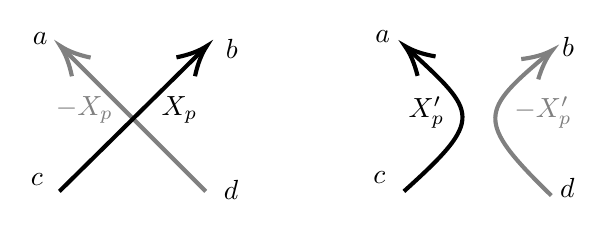
\begin{tikzpicture}[x=0.75pt,y=0.75pt,yscale=-1,xscale=1]
%uncomment if require: \path (0,109); %set diagram left start at 0, and has height of 109

%Straight Lines [id:da7979059503936952] 
\draw [color={rgb, 255:red, 128; green, 128; blue, 128 }  ,draw opacity=1 ][line width=1.5]    (39.62,19.12) -- (107.5,87) ;
\draw [shift={(37.5,17)}, rotate = 45] [color={rgb, 255:red, 128; green, 128; blue, 128 }  ,draw opacity=1 ][line width=1.5]    (14.21,-6.37) .. controls (9.04,-2.99) and (4.3,-0.87) .. (0,0) .. controls (4.3,0.87) and (9.04,2.99) .. (14.21,6.37)   ;
%Straight Lines [id:da7279842833116223] 
\draw [color={rgb, 255:red, 0; green, 0; blue, 0 }  ,draw opacity=1 ][line width=1.5]    (105.86,19.11) -- (37,87) ;
\draw [shift={(108,17)}, rotate = 135.41] [color={rgb, 255:red, 0; green, 0; blue, 0 }  ,draw opacity=1 ][line width=1.5]    (14.21,-6.37) .. controls (9.04,-2.99) and (4.3,-0.87) .. (0,0) .. controls (4.3,0.87) and (9.04,2.99) .. (14.21,6.37)   ;
%Curve Lines [id:da5605408166706283] 
\draw [color={rgb, 255:red, 0; green, 0; blue, 0 }  ,draw opacity=1 ][line width=1.5]    (203,87) .. controls (242.2,51.72) and (238.18,49.09) .. (205.53,18.88) ;
\draw [shift={(203.5,17)}, rotate = 402.85] [color={rgb, 255:red, 0; green, 0; blue, 0 }  ,draw opacity=1 ][line width=1.5]    (14.21,-6.37) .. controls (9.04,-2.99) and (4.3,-0.87) .. (0,0) .. controls (4.3,0.87) and (9.04,2.99) .. (14.21,6.37)   ;
%Curve Lines [id:da8925010918239024] 
\draw [color={rgb, 255:red, 128; green, 128; blue, 128 }  ,draw opacity=1 ][line width=1.5]    (274,89) .. controls (236.76,52.74) and (239.86,48.17) .. (272.47,20.71) ;
\draw [shift={(274.5,19)}, rotate = 499.95] [color={rgb, 255:red, 128; green, 128; blue, 128 }  ,draw opacity=1 ][line width=1.5]    (14.21,-6.37) .. controls (9.04,-2.99) and (4.3,-0.87) .. (0,0) .. controls (4.3,0.87) and (9.04,2.99) .. (14.21,6.37)   ;

% Text Node
\draw (23,9.4) node [anchor=north west][inner sep=0.75pt]    {$a$};
% Text Node
\draw (116,12.4) node [anchor=north west][inner sep=0.75pt]    {$b$};
% Text Node
\draw (22,77.4) node [anchor=north west][inner sep=0.75pt]    {$c$};
% Text Node
\draw (115,80.4) node [anchor=north west][inner sep=0.75pt]    {$d$};
% Text Node
\draw (85,40) node [anchor=north west][inner sep=0.75pt]  [color={rgb, 255:red, 0; green, 0; blue, 0 }  ,opacity=1 ]  {$X_p$};
% Text Node
\draw (34,40) node [anchor=north west][inner sep=0.75pt]  [color={rgb, 255:red, 128; green, 128; blue, 128 }  ,opacity=1 ]  {$-X_p$};
% Text Node
\draw (188,8.4) node [anchor=north west][inner sep=0.75pt]    {$a$};
% Text Node
\draw (278,11.4) node [anchor=north west][inner sep=0.75pt]    {$b$};
% Text Node
\draw (187,76.4) node [anchor=north west][inner sep=0.75pt]    {$c$};
% Text Node
\draw (277,79.4) node [anchor=north west][inner sep=0.75pt]    {$d$};
% Text Node
\draw (204,40) node [anchor=north west][inner sep=0.75pt]  [color={rgb, 255:red, 0; green, 0; blue, 0 }  ,opacity=1 ]  {$X'_p$};
% Text Node
\draw (255,40) node [anchor=north west][inner sep=0.75pt]  [color={rgb, 255:red, 128; green, 128; blue, 128 }  ,opacity=1 ]  {$-X'_p$};


\end{tikzpicture}
    \caption{$X_{p}$ and $X'_{p}$}
    \label{fig:crossing}
\end{figure}

Next we show that a generating set of $R(D)$ can be given by considering a spanning tree of the Seifert graph of $D$.
For each crossing $p$ of $D$, we define $X_{p}, X'_{p} \in R(D)$ by
\begin{align*}
    X_p &= x_b - x_c = -(x_a - x_d), \\
    X'_p &= x_a - x_c = -(x_b - x_d),
\end{align*}
where $a, b$ are outgoing edges at $p$ and $c,d$ are incoming edges at $p$, and $a, c$ are placed to the left of $p$ (see \Cref{complex,fig:crossing}).

\begin{lemma}[\cite{Nak20}]\label{treebasislem}
    Let $T$ be a spanning tree of the Seifert graph of $D$, and $S$ the set of crossings in $D$ corresponding to the edges of $T$.
    Then, $\mathcal{X}_T = \{X_p\}_{p \in S} \cup \{X'_p\}_{p \notin S}$ is an algebraically independent generating set of $R(D)$.
\end{lemma}

\begin{figure}
    \centering
    \tikzset{every picture/.style={line width=0.75pt}} %set default line width to 0.75pt        

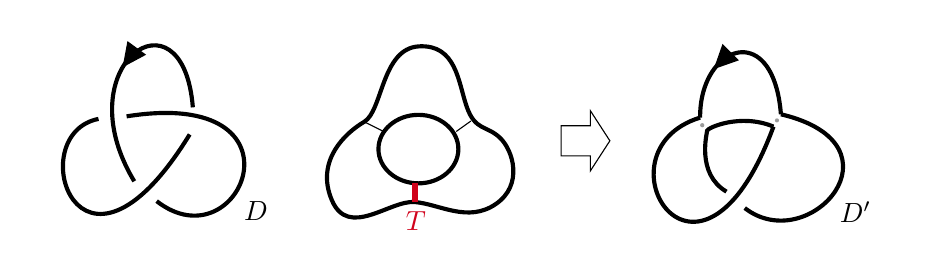
\begin{tikzpicture}[x=0.75pt,y=0.75pt,yscale=-1,xscale=1]
%uncomment if require: \path (0,109); %set diagram left start at 0, and has height of 109

\clip (0,0) rectangle (420,100);

%Curve Lines [id:da8161601596307948] 
\draw [line width=1.5]    (79.58,38.39) .. controls (74.8,-21.4) and (17.36,17.84) .. (51.36,74.01) ;
\draw [shift={(45.72,19.12)}, rotate = 306.15999999999997] [fill={rgb, 255:red, 0; green, 0; blue, 0 }  ][line width=0.08]  [draw opacity=0] (11.61,-5.58) -- (0,0) -- (11.61,5.58) -- cycle    ;
%Curve Lines [id:da5647400415250446] 
\draw [line width=1.5]    (62.15,83.58) .. controls (102.85,115.24) and (138.02,28.21) .. (47.66,42.73) ;
%Curve Lines [id:da13846906868786935] 
\draw [line width=1.5]    (34.13,43.95) .. controls (-3.3,51.35) and (24.68,138.29) .. (78.06,51.44) ;
%Curve Lines [id:da237486702787586] 
\draw [line width=1.5]    (362.91,41.73) .. controls (362.73,39.45) and (362.47,37.31) .. (362.15,35.31) .. controls (356.65,1.83) and (331.88,7.57) .. (325.49,31.04) .. controls (324.49,34.73) and (323.94,38.84) .. (323.99,43.32) ;
%Curve Lines [id:da6079162773576449] 
\draw [line width=1.5]    (345.48,86.91) .. controls (376.67,111) and (424.67,56.33) .. (362.91,41.73) ;
%Curve Lines [id:da012895447238909785] 
\draw [line width=1.5]    (323.99,43.32) .. controls (271.33,59.67) and (323.33,145) .. (359.33,47.67) ;
%Curve Lines [id:da4889524635526027] 
\draw [line width=1.5]    (359.33,47.67) .. controls (343.33,41) and (327.33,48.33) .. (327.33,49.67) .. controls (327.33,51) and (322,70.33) .. (336.67,79) ;
%Flowchart: Connector [id:dp9085114377251573] 
\draw  [draw opacity=0][fill={rgb, 255:red, 155; green, 155; blue, 155 }  ,fill opacity=1 ] (323.97,46.98) .. controls (323.97,46.42) and (324.43,45.96) .. (324.99,45.96) .. controls (325.55,45.96) and (326.01,46.42) .. (326.01,46.98) .. controls (326.01,47.54) and (325.55,48) .. (324.99,48) .. controls (324.43,48) and (323.97,47.54) .. (323.97,46.98) -- cycle ;
%Flowchart: Connector [id:dp9045304281632592] 
\draw  [draw opacity=0][fill={rgb, 255:red, 155; green, 155; blue, 155 }  ,fill opacity=1 ] (360,44.67) .. controls (360,44.11) and (360.45,43.67) .. (361,43.67) .. controls (361.55,43.67) and (362,44.11) .. (362,44.67) .. controls (362,45.22) and (361.55,45.67) .. (361,45.67) .. controls (360.45,45.67) and (360,45.22) .. (360,44.67) -- cycle ;
%Shape: Polygon Curved [id:ds49799004625007537] 
\draw  [line width=1.5]  (162.13,45.37) .. controls (171.07,40.12) and (170.5,10) .. (188.5,9) .. controls (206.5,8) and (207.42,26.18) .. (211.5,38) .. controls (215.58,49.82) and (221.05,46.9) .. (227.5,53) .. controls (233.95,59.1) and (238.94,75.83) .. (225.5,85) .. controls (212.06,94.17) and (198.5,85) .. (186.5,84) .. controls (174.5,83) and (154.5,102) .. (146.5,83) .. controls (138.5,64) and (153.18,50.62) .. (162.13,45.37) -- cycle ;
%Shape: Ellipse [id:dp8656777374199306] 
\draw  [line width=1.5]  (169,58.5) .. controls (169,49.39) and (177.62,42) .. (188.25,42) .. controls (198.88,42) and (207.5,49.39) .. (207.5,58.5) .. controls (207.5,67.61) and (198.88,75) .. (188.25,75) .. controls (177.62,75) and (169,67.61) .. (169,58.5) -- cycle ;
%Straight Lines [id:da1480688684375554] 
\draw    (162.13,45.37) -- (171.5,50) ;
%Straight Lines [id:da3873077880987402] 
\draw    (213.5,45) -- (206.5,50) ;
%Straight Lines [id:da043234858474899274] 
\draw [color={rgb, 255:red, 208; green, 2; blue, 27 }  ,draw opacity=1 ][line width=2.25]    (186.5,75) -- (186.5,84) ;
%Straight Lines [id:da23585575290034488] 
\draw [line width=1.5]    (335.5,15) -- (333.33,17.17) ;
\draw [shift={(330.5,20)}, rotate = 315] [fill={rgb, 255:red, 0; green, 0; blue, 0 }  ][line width=0.08]  [draw opacity=0] (11.61,-5.58) -- (0,0) -- (11.61,5.58) -- cycle    ;
%Right Arrow [id:dp28729390632428686] 
\draw   (257,47.25) -- (271.1,47.25) -- (271.1,40) -- (280.5,54.5) -- (271.1,69) -- (271.1,61.75) -- (257,61.75) -- cycle ;

% Text Node
\draw (103,82.4) node [anchor=north west][inner sep=0.75pt]    {$D$};
% Text Node
\draw (390,82.4) node [anchor=north west][inner sep=0.75pt]    {$D'$};
% Text Node
\draw (181,87.4) node [anchor=north west][inner sep=0.75pt]    {$\textcolor[rgb]{0.82,0.01,0.11}{T}$};


\end{tikzpicture}
    \caption{$D, T$ and $D'$}
    \label{fig:treebasislem}
\end{figure}

\begin{proof}
    Working over $\QQ$ allows us to have the equation
    \[
    \QQ[x_1, \ldots , x_m] = \QQ[x_1-x_2,\ x_2-x_3,\ \ldots,\ x_{m-1}-x_m,\ x_1+\cdots+x_m].
    \]
    Thus it follows that $R(D)$ is generated by elements of the form $x_e - x_f$, where $e, f$ are edges of $G(D)$.
    Since $|\mathcal{X}_T| = n$, it is enough to show that each $x_e - x_f$ can be written as a linear sum of elements in $\mathcal{X}_T$.
    Since $D$ is connected, by resolving all crossings in $D$ which are not in $S$, we obtain a diagram $D'$ of the trivial knot (see \Cref{fig:treebasislem} for an easy case).
    There is a unique oriented path $\gamma$ in $G(D')$ from $f$ to $e$, which may be also regarded as a path in $G(D)$.
    Trace $\gamma$ from $x_f$ to $x_e$, and each time $\gamma$ passes a crossing $p$ in $D$, take a term $\pm X_p$ or $\pm X'_p$ according to how $\gamma$ passes $p$ (see \Cref{fig:crossing}).
    It is obvious that these terms belong to $\mathcal{X}_T$ and that the sum gives $x_e-x_f$.
\end{proof}

\subsection{Reinterpretation as cube complexes} \label{subsec:double-cube-cpx}

Next we reinterpret the chain complex $C(D)$ given in \Cref{sec:prelim} as a ``double cube complex". Precise statement follows.

The \textit{$n$-cube} is a poset $\{0, 1\}^n$ with the product order of $0 < 1$, considered as a category.
An object $v \in \{0, 1\}^n$ is called a \textit{vertex}, and the Manhattan norm of $v$ is denoted by $|v| = v_1 + \cdots + v_n$. A morphism $v \to w$ such that $|v| + 1 = |w|$ is denoted $v \to_1 w$ and called an \textit{edge}. Define vertices $\bar{0} = (0, \ldots, 0)$ and $\bar{1} = (1, \ldots, 1)$.

\begin{figure}
    \centering
    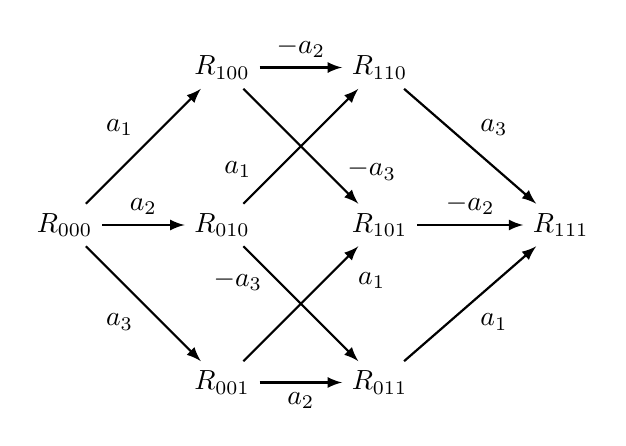
\begin{tikzpicture}[auto]
    \node (v0) at (-3.5,0.5) {$R_{000}$};
    \node (v1) at (-1.5,2.5) {$R_{100}$};
    \node (v2) at (-1.5,0.5) {$R_{010}$};
    \node (v3) at (-1.5,-1.5) {$R_{001}$};
    \node (v4) at (0.5,2.5) {$R_{110}$};
    \node (v5) at (0.5,0.5) {$R_{101}$};
    \node (v6) at (0.5,-1.5) {$R_{011}$};
    \node (v7) at (2.8,0.5) {$R_{111}$};
    \draw[-latex, thick] (v0) to node {$a_1$} (v1);
    \draw[-latex, thick] (v0) to node {$a_2$} (v2);
    \draw[-latex, thick] (v0) to node[swap] {$a_3$} (v3);
    \draw[-latex, thick] (v1) to node {$-a_2$} (v4);
    \draw[-latex, thick] (v1) edge (v5);
    \draw[-latex, thick] (v2) edge (v4);
    \draw[-latex, thick] (v2) edge (v6);
    \draw[-latex, thick] (v3) edge (v5);
    \draw[-latex, thick] (v3) to node[swap] {$a_2$} (v6);
    \draw[-latex, thick] (v4) to node {$a_3$} (v7);
    \draw[-latex, thick] (v5) to node {$-a_2$} (v7);
    \draw[-latex, thick] (v6) to node[swap] {$a_1$} (v7);
    \node at (0.4,-0.2) {$a_1$};
    \node at (0.4,1.2) {$-a_3$};
    \node at (-1.3,-0.2) {$-a_3$};
    \node at (-1.3,1.2) {$a_1$};
\end{tikzpicture}

    \caption{A cube complex with factors $(a_1, \ldots, a_n)$.}
    \label{fig:cube-complex}
\end{figure}

Let $\mathcal{A}$ be an additive category.
\begin{definition}
    For $n \geq 0$, an \textit{$n$-cube in $\mathcal{A}$} is a functor $\mathcal{C}\colon \{0, 1\}^n \to \mathcal{A}$.
\end{definition}

Given an $n$-cube $\mathcal{C}$ in $\mathcal{A}$,
one obtains a \textit{cube complex} $(C^*, d^*)$ in $\mathcal{A}$ with 
\[
    C^i = \bigoplus_{|v| = i} \mathcal{C}(v)
\]
and differentials
\[
    d^i = \sum_{\substack{|v| = i,\\ e\colon v \to w}} s(e)\mathcal{C}(e),
\]
by choosing $s(e) \in \{\pm 1\}$ for each edge $e$ of the cube so that for any square consisting of four edges $e_1,\ldots,e_4$, we have $s(e_1) \cdots s(e_4) = -1$.

\begin{remark}
    The isomorphism class of the above cube complex is independent of the choice of $s$.
\end{remark}

Now we put $C(D)$ in this framework. First we will ignore the original homological gradings, and lately relate them with the newly introduced gradings. 
%
We recall that $C(D)$ is a tensor product of (vertical) two-terms complexes of (horizontal) complexes. Hence $C(D)$ can be regarded as a cube complex of complexes. We write 
\[
    C(D) = \bigoplus_{v \in \{0, 1\}^n} C^*_v(D),
\]
where $C^*_v(D)$ is the complex at a vertex $v \in \{0, 1\}^n$, called the \textit{horizontal complex} of $D$ at $v$.
Since $C^*_v(D)$ is also a tensor product of two-terms complex over $R(D)$, it can be regarded as a cube complex again. We write
\[
    C^*_v(D) = \bigoplus_{h \in \{0, 1\}^n} R_{v, h}(D),
\]
where $R_{v, h}(D)$ is the module at a vertex $h \in \{0, 1\}^n$, and it is indeed a shifted copy of $R(D)$. The horizontal differential 
\[
    d_H: C^*_v(D) \rightarrow C^{*+1}_v(D)
\]
has the following form.
For each standard unit vector $e_i$ of $\RR^n$, there exists an element $a_i$ of $R(D)$ such that for any edge $v \to_1 w$ in the direction of $e_i$ in the $n$-cube, the corresponding map $R_{v,h}(D) \to R_{w,h}(D)$ summed in $d_H$ is the multiplication map by $a_i$ as specified by the horizontal arrows of \Cref{complex} according to $v$ (with some appropriate sign assignment). We call $a_1, \ldots, a_n$ the \textit{factors} of $C^*_v(D)$ (see \Cref{fig:cube-complex}).

By taking the homology with respect to $d_H$, we get a cube complex of homologies
\[
    \bigoplus_{v \in \{0, 1\}^n} H^*(C_v(D), d_H)
\]
with differential $(d_V)_*$. Then it is obvious that $\Hhat(D)$ is given by the homology of this complex
\[
    \Hhat(D) = H(\oplus_v (H(C_v(D), d_H), (d_V)_*).
\]

The homological bigrading $(\alpha, \beta)$ of the double cube complex $C(D)$ correspond to the original bigrading $(j, k)$ as
\[
    (\alpha, \beta) = \frac{1}{2}(j - j_0,\ k - k_0)
\]
where $(j_0, k_0)$ is the (original) homological bidegree of the module $R_{\bar{0}, \bar{0}}(D)$ placed at $(v, h) = (\bar{0}, \bar{0})$. For later use, let $i_0$ denote the $q$-grading shift of $R_{\bar{0}, \bar{0}}(D)$. Then from \Cref{complex} we have 
%
\begin{equation} \label{eq:ijk0}
    (i_0, j_0, k_0) = (2n^+, -2n, -2n^+)
\end{equation}
%
where $n_+$ and $n_-$ are the number of positive and negative crossings of $D$ respectively.

\subsection{Slicing by $q$-degrees} 

As described in \Cref{treebasislem}, the ring $R(D)$ can be represented by a multivariate polynomial ring $\QQ[X_i]$ with $n$ variables, so we have a homogeneous decomposition of $R(D)$ as a $\QQ$-vector space
\[
    R(D) \isom \QQ(1) \oplus \QQ(X_i)_{1 \leq i \leq n}  \oplus \QQ(X_i X_j)_{1 \leq i \leq j \leq n} \cdots.
\]
Let $i_{v, h} \in \ZZ$ be the $q$-grading shift of $R_{v, h}(D) = R(D)\{i_{v, h}\}$. Decompose $R_{v, h}(D)$ as 
\[
    R_{v, h}(D) = \bigoplus_{l = -\infty}^\infty V_{l, v, h}(D)
\]
so that each $V_{l, v, h}(D)$ is homogeneous of $q$-degree $2(l + |h|) + i_0$. It is generated by monomials 
% $X_{i_1} \cdots X_{i_e}$ 
of degree (in the usual sense) 
%
\begin{equation} \label{eq:monomial-degree}
    e(l, v, h) = l + |h| + \frac{i_0 - i_{v, h}}{2}.
\end{equation}
%
Now define 
\[
    C_l(D) = \bigoplus_{v, h} V_{l, v, h}(D)
\]
then it is obvious that both $d_H, d_V$ are closed in $C_l(D)$.  Regarding $C(D)$ as a chain complex over $\QQ$, we get a decomposition
\[
    C(D) = \bigoplus_{l = -\infty}^\infty C_l(D).
\]
We call each subcomplex $C_l(D)$ the \textit{level-$l$ slice} of $C(D)$. Note that the decomposition is defined so that $V_{l, \bar{0}, \bar{0}}(D)$ is generated by monomials of degree $e = l$. 

\begin{lemma}
    $C_l(D) = 0$ for $l < -2n$.
\end{lemma}

\begin{proof}
    The claim is clear since $e$ is non-decreasing with respect to $v, h$ and $e(l, \bar{1}, \bar{1}) = l + 2n$.
\end{proof}

From the previous arguments, it is obvious that each $C_l(D)$ may also be regarded as a double cube complex. Define the \textit{level-$l$ slice} $C_{l, v}(D)$ of the horizontal complex $C_v(D)$ at $v \in \{0, 1\}^n$ by
\[
    C_{l, v}(D) = \bigoplus_{h \in \{0, 1\}^n} V_{l, v, h}(D).
\]
Then we get a decomposition
\[
    \Hhat(D) = \bigoplus_{l = -2n}^\infty \Hhat_l(D),
\]
where 
\[
    \Hhat_l(D) = H(\oplus_v (H(C^*_{l, v}(D), d_H), (d_V)_*).
\]

We claim that each $\Hhat_l(D)$ is algorithmically computable. To take the homology twice, we find a basis on each chain group $C^i = C^i_{l, v}(D)$ that gives a decomposition
\[
    C^i = H^i \oplus B^i \oplus (d^i_H)^{-1}(B^{i + 1})
\]
so that we get representative cycles of the generators of $H^i = H^i(C^*_{l, v}(D))$ and that the secondary homology computation can be done on the chain level. This is achieved by standard methods such as the Gaussian elimination. 

\begin{proposition}
    For a link diagram $D$, the homology $\Hhat(D)$ has a decomposition
    \[
        \Hhat(D) = \bigoplus_{l = -2n}^{\infty} \Hhat_l(D)
    \]
    where each summand $\Hhat_l(D)$ can be computed algorithmically. Moreover for each triple degree $(i, j, k)$ we have 
    %
    \begin{equation} \label{eq:Hijk}
        \Hhat^{i, j, k}(D) = H^\beta(\oplus_v (H^\alpha(C^*_{v, l}(D), d_H), (d_V)_*)
    \end{equation}
    %
    where
    %
    \[
        (l, \alpha, \beta) = \frac{1}{2}((i - i_0) - (j - j_0),\ j - j_0,\ k - k_0)
    \]
    and $(i_0, j_0, k_0)$ are given as in \eqref{eq:ijk0}. Similar statement holds for $\Hbar(D)$. \qed
\end{proposition}

Now we restrict to the case where $D$ is a knot diagram, and in particular where it is a braid closure. In such case, it is well-known that $\Hbar(D)$ is finite dimensional \cite{Ras15}. In order to perform the actual calculation, we must specify an actual upper bound for the level $l$.

\begin{proposition} \label{prop:finiteness}
    If $K$ is a knot with braid closure diagram $D$, then
    \[
        \Hbar(K) \isom \bigoplus_{l = -2n}^{-n} \Hbar_l(D).
    \]
    Moreover, $\Hbar(K)$ can be obtained from the computations of $\Hbar^{i, j, k}(D)$ within the following ranges:
    \begin{align*}
        i &\in [-n + s - 1, 0], \tag{1}\\
        j &\in [w - s + 1, w + s - 1], \tag{2}\\
        k,\ k + 2i &\in [-n + s - 1, n - s + 1]. \tag{3}
    \end{align*}
\end{proposition}

\begin{proof}
    From \Cref{prop:MFW-ineq,prop:morton} and equation \eqref{eq:Hbar-def}, it follows that $\Hbar_l(D)$ is supported in 
    \begin{align*}
        2l 
        &= (i - i_0) - (j - j_0) \\ 
        &\leq \{ (n - s + 1) - (-w + s - 1) - 2n^+ \}\\
        &\quad - \{(w - s + 1) - (w + s - 1) - (-2n)\}\\
        &= -2n.
    \end{align*}
    For the latter statement: (1) the lower bound is given by the Morton bound (\Cref{prop:morton}), and from \Cref{prop:q-sym} it suffices to compute $H^{i, *, *}(D)$ within $i \leq 0$.
    (2) This is exactly \Cref{prop:MFW-ineq}.
    (3) The lower bound of $k$ is obvious from the definition of $C(D)$, and from \Cref{prop:duality} we also have the upper bound. From \Cref{prop:q-sym}, $k + 2i$ must also lie in this range.
\end{proof}

\subsection{Exclusion of variables}

As apparent from \eqref{eq:monomial-degree}, the number of generators increases combinatorially as $l$ increases. In order to reduce the computational cost, we use the process called ``exclusion of variables" as described in \cite[Lemma 3.8]{Ras15}. 

Again we assume $D$ is a link diagram. Put $R = R(D)$. Take any $v \in \{0, 1\}^n$ and consider the horizontal cube complex $C = C_v(D)$. Take any factor $f \in R$ of $C$. Note that $f$ is either linear or quadratic.

After choosing an appropriate sign assignment, $C$ may be regarded as the mapping cone of the endomorphism 
\[
    C' \xrightarrow{f} C'
\]
of an $n-1$ dimensional cube complex $C'$. Let $d, d'$ denote the differentials of $C, C'$ respectively. The complex $C$ is isomorphic to $C' \oplus C'$ as an $R$-module, and we can write
\[
    d(x_0, x_1) = (-d'x_0, fx_0 + d'x_1).
\]

Now $f$ is monic with respect to some variable $X_k$. Define
\[
R_0 = \QQ[X_1, \ldots \widehat{X_k}, \ldots, X_n].
\]
Let $\pi \colon R \rightarrow R_1 = R/(f)$ be the quotient map, $\iota \colon R_1 \rightarrow R$ be the map that sends any residue class $[g] \in R_1$ to the remainder of $g$ by $f$ with respect to the variable $X_k$.
We note that $\pi$ and $\iota$ are homomorphisms of modules over $R$ and $R_0$ respectively.
Let $C'' = C' \otimes_R R_1$, and let $d''$ be the differential of $C''$. Two chain maps $\phi \colon C \rightarrow C''$ and $\psi \colon C'' \rightarrow C$ over $R_0$ are given by
\[
    \phi(x_0, x_1) = \pi(x_1),
\]
and
\[
    \psi(y) = \left(\frac{\iota(d''y) - d'\iota(y)}{f},\  \iota(y)\right),
\]
and it is not hard to verify that $\psi \phi \htpy \id_C$ and $\phi \psi = \id_{C''}$.
The complex $C''$ admits the obvious triple grading so that both $\phi, \psi$ are degree preserving. Thus the two maps restrict as chain homotopy equivalences between the two sliced complexes $C_l$ and $C''_l$. The effect is that $H(C_l) \cong H(C''_l)$ can be computed with fewer generators, which is drastic when $l$ becomes large. 

Furthermore, this process of reduction can be repeated for other directions as long as the target variable is algebraically independent in the base ring. When $f$ is linear, we have $R_1 \isom R_0$ and all other variables remain independent. When $f$ is quadratic, then $R_1 \isom R_0 \otimes_\QQ \QQ\{1, X_k\}$ as $\QQ$-vector spaces, and the variables that does not appear in the coefficients of $f$ remains independent.

In particular, when all factors $f$ of $C$ are linear, then the exclusion can be continued until the differential becomes trivial. In general, to exclude the variables as much as possible, it is preferable to perform exclusions on linear polynomials first, and then on the remaining quadratics. 

For the computation of $\Hbar(D)$, we can replace each horizontal complex $C_{l, v}$ with a reduced one, compute those homologies, and replace the differential $(d_V)_*$ on the vertical complex with $(\phi_{v'} \circ d_V \circ \psi_v)_*$ for each edge $v \rightarrow v'$. 

\subsection{Overall procedure}

We summarize the overall procedure for computing (the dimensions of) the reduced HOMFLY homology $h^{i, j, k} = \{\dim \Hbar^{i, j, k}(K)\}_{i, j, k}$ of a knot $K$.

\begin{algorithm}\label{algo:basic}
    Given a braid closure diagram $D$ of a knot $K$, 
    \begin{enumerate}
        \item Compute the Seifert graph $G(D)$ and find a spanning tree $T$ of $G(D)$. 
        
        \item Using $T$, identify the edge ring $R(D)$ as a multivariate polynomial ring, and represent both $d_H$ and $d_V$ as $n$-tuples of polynomials in $R(D)$ as in the proof of \Cref{treebasislem}.
        
        \item For each $(l, \alpha, \beta)$ in $[-2n, -n] \times [0, n] \times [0, n]$:
        \begin{enumerate}
            \item Convert $(l, \alpha, \beta)$ to $(i, j, k)$. Skip to the next iteration if $(i, j, k)$ is not in the range of \Cref{prop:finiteness}.
            
            \item Setup the generators of the level-$l$ horizontal complex $C_l(D)$.
            
            \item Perform exclusion of variables on $C_l(D)$ to get a reduced complex together with the chain homotopy equivalences. 

            \item Compute $h^{i, j, k} = \dim \Hbar^{i, j, k}(D)$ from \eqref{eq:Hijk}, with the horizontal complexes replaced with the reduced ones. 
            
            \item Assign $h^{-i, j, k + 2i} = h^{i, j, k}$ if $i < 0$.
        \end{enumerate}
        \item Return $h$.
    \end{enumerate}
\end{algorithm}

Reusable data should be cached within the iteration. Further improvement can achieved by concerning mirrors of knots. To explain this, assume that $D$ has only one crossing $p$. Recall that the vertex module $V_{l, v, h}(D)$ at $(v, h) \in \{0, 1\}^2$ is spanned by the monomials of degree given  by \eqref{eq:monomial-degree}. From \Cref{complex}, we see that $e(l, 1, 0) = e(l, 0, 1) = e(l, 0, 0) + 1$ if $p$ is positive, and $e(l, 1, 0) = e(l, 0, 1) = e(l, 0, 0)$ if $p$ is negative (in both cases $e(l, 1, 1) = e(l, 0, 0) + 1$). This means that $C_l(D)$ has a smaller generating set when $p$ is negative. In general if $w(D) > 0$, then $C_l(m(D))$ has a smaller generating set than $C_l(D)$. This difference becomes intense as $n$ increases. Thus the improved version is:

\begin{algorithm}\label{algo:mirror}
    Given a braid closure representative $D$ of a knot $K$, \begin{enumerate}
        \item If $w(D) \leq 0$, compute and return $h(D)$ by \Cref{algo:basic}.
        \item Otherwise, compute $h(m(D))$ by \Cref{algo:basic} and return its dual.
    \end{enumerate}
\end{algorithm}
\section{Skyline Computation Over Categorical Attributes}\label{sec:3}
Without loss of generality, for ease of explanation, we consider a relation with Boolean attributes, i.e., categorical attributes with domain size 2. We shall discuss the extensions of the algorithms for categorical attributes with larger domains later in this section.

Throughout this section, we consider the case in which precomputed indices are not available. First, we exploit the categorical characteristics of attributes by designing a tree data structure that can perform efficient {\em dominance} operations. Specifically, given a new tuple $t$, the tree supports three primitive operations -- i) INSERT($t$): inserts a new tuple $t$ to the tree, ii) IS-DOMINATED($t$): checks if tuple $t$ is dominated by any tuple in the tree, and iii) PRUNE-DOMINATED-TUPLES($t$): deletes the tuples dominated by $t$ from the tree. In Appendix \ref{ap:tree-optimizations}, we further improve the performance of these basic operations by proposing several optimization techniques. Finally, we propose two algorithms ST-S (Skyline using Tree Sorting-based) and ST-P (Skyline using Tree Partition-based) that incorporate the tree structure to state-of-art sorting- and partition-based algorithms.


\subsection{Organizing Tuples Tree}\label{subsec:tree}
\vspace{1mm}
\noindent{\bf Tree structure:} We use a binary tree to store tuples in the candidate skyline set. Consider an ordering of all attributes in $\mathcal{Q} \subseteq \mathcal{A}$, e.g., $[A_1, A_2, \ldots, A_{m'}]$.
In addition to tuple attributes, we enhance each tuple with a score, assessed using a function $F(\cdot)$. This score assists in improving performance during identification of the dominated tuples or while conducting the dominance check. The proposed algorithm is agnostic to the choice of $F(\cdot)$; the only requirement is that the function does not assign a higher score to a dominated tuple compared to its dominator.
The structure of the tree for Example~\ref{exmp:ST} is depicted in Figure~\ref{fig:tree}. The tree has a total of 5 ($=m'+ 1$) levels, where the $i$'th level ($1 \leq i \leq m'$) represents attribute $A_i$. The left (resp. right) edge of each internal node represents value 0 (resp. 1). Each path from the root to a leaf represents a specific assignment of attribute values. The leaf nodes of the tree 
store two pieces of information: i) $score$: the score of the tuple mapped to that node, and ii) \textit{tupleID List}: list of ids of the tuples mapped to that node. Note that all the tuples that are mapped to the same leaf node in the tree have the same attribute value assignment, i.e. have the same score.
Moreover, the attribute values of a tuple $t$ can be identified by inspecting the path from the root to a leaf node containing $t$. Thus, there is no requirement to store the attribute values of the tuples in the leaf nodes.
Only the leaf nodes that correspond to an actual tuple are present in the tree. 

\begin{exmp}\label{exmp:ST} 
As a running example through out this section, consider the relation $D$ with $n=5$ non-dominated tuples where its projection on $\mathcal{Q}=\{A_1,A_2,A_3,A_4\}$ is depicted in Table~\ref{tab:skylineTreeRunningExample}. 
The last column of the table presents the score of each tuple, utilizing the function $F(\cdot)$  provided in Equation~\ref{eq:score}.
\begin{align}\label{eq:score}
F(t_{\mathcal{Q}}) = \sum_{A_i \in \mathcal{Q}} 2^{i-1} \cdot t[A_i]
\end{align}
\end{exmp}



\begin{table}[!t]
\centering
\caption{Example~\ref{exmp:ST} relation}\label{tab:skylineTreeRunningExample}
\begin{tiny}
\begin{tabular}{cccccc}
    \hline 
    $tupleID$ & $A_1$ & $A_2$ & $A_3$ & $A_4$ & $Score$\\
    \hline 
    $t_1$ & 1 & 1 & 0 & 0 & 12\\
    \hline
    $t_2$ & 0 & 0 & 1 & 1 & 3\\
    \hline
    $t_3$ & 0 & 1 & 1 & 0 & 6\\
    \hline
    $t_4$ & 1 & 0 & 0 & 1 & 9\\
    \hline
    $t_5$ & 1 & 0 & 1 & 0 & 10\\
    \hline
\end{tabular}
\end{tiny}
\end{table}

\begin{figure*}[!t]
\begin{minipage}[t]{0.23\linewidth}
\centering
    \includegraphics[scale=0.80]{figures/SkylineTree.pdf}
    %\vspace{-8mm}
    \caption{Tree structure for relation in Example~\ref{exmp:ST}}
    \label{fig:tree}
\end{minipage}
\hspace{1mm}
\begin{minipage}[t]{0.23\linewidth}
\centering
    \includegraphics[scale=0.80]{figures/SkylineTreeDominate.pdf}
    %\vspace{-8mm}
    \caption{Prune dominated tuples}
    \label{fig:treePruneDominatedTuples}
\end{minipage}
\hspace{1mm}
\begin{minipage}[t]{0.23\linewidth}
\centering
    \includegraphics[scale=0.80]{figures/SkylineTreeDominateAfter.pdf}
    %\vspace{-8mm}
    \caption{Tree after removing dominated tuples}
    \label{fig:treePruneDominatedTuplesAfter}
\end{minipage}
\hspace{1mm}
\begin{minipage}[t]{0.23\linewidth}
\centering
    \includegraphics[scale=0.80]{figures/SkylineTreeDominated.pdf}
    %\vspace{-8mm}
    \caption{Check if tuple $t$ is dominated}
    \label{fig:treeCheckIfDominated}
\end{minipage}
\end{figure*}


\vspace{1mm}
\noindent{\bf INSERT($t$):} In order to insert a tuple $t$ into the tree, we start from the root. At level $i$ $(1 \leq i \leq m')$, we check the corresponding attribute value, $t[A_i]$. If $t[A_i] = 0$ (resp. $t[A_i] = 1$) and the left (resp. right) child of current node already exists in the tree, we simply follow the left (resp. right) child. Otherwise, we first have to create a new tree node as left (resp. right) child before traversing it. After reaching the leaf node at level $m'+1$, the $tupleID$ of $t$ is appended to \textit{tupleID List} and the $score$ value is assigned to newly constructed leaf.

\begin{algorithm}[!htb]
\caption{{\bf INSERT}}
\begin{algorithmic}[1]
\label{alg:insertTuple}
\STATE {\bf Input:} Tuple $t$, Node $n$, Level $l$, Query $\mathcal{Q}$;
%\STATE {\bf if} $n$ is $leaf$ node:
\STATE {\bf if} $l == |\mathcal{Q}| + 1$:
    \STATE \hindent {\bf if} $n.score$ is None: $n.score = score(t)$
    \STATE \hindent Append $t[tupleID]$ to $n.tupleIDList$
\STATE {\bf else}:
    \STATE \hindent {\bf if} $t[A_l]==0$:
        \STATE \hindent[2] {\bf if} $n.left$ is $None$:
           % \STATE \hindent[3] Create $left$ child of $t$
           \STATE \hindent[3] temp = {\it New} Node();
           \STATE \hindent[3] $t.left$ = temp;
        \STATE \hindent[2] INSERT($t$, $n.left$, $l+1$)
    \STATE \hindent {\bf if} $t[A_l]==1$:
        \STATE \hindent[2] {\bf if} $n.right$ is $None$:
           % \STATE \hindent[3] Create $right$ child of $t$
           \STATE \hindent[3] temp = {\it New} Node();
           \STATE \hindent[3] $t.right$ = temp;
        \STATE \hindent[2] INSERT($t$, $n.right$, $l+1$)
\end{algorithmic}
\end{algorithm}

\vspace{1mm}
\noindent{\bf PRUNE-DOMINATED-TUPLES($t$):} The pruning algorithm to delete from the tree, tuples dominated by $t$, is recursively developed as follows: We start from the root node of the tree. If $t[A_1] = 1$, we search both the left and right subtree. Otherwise, only the left child is selected. This is because if $t[A_1] = 1$, a tuple $t'$ dominated by $t$ can assume value  0 or 1 on attribute $A_1$. On the other hand, $t$ cannot dominate a tuple $t'$ if $t[A_1] = 0$ and $t'[A_1] = 1$. We follow the same approach at each internal node visited by the algorithm - at level $i$ $(1 \leq i \leq m)$, value of $t[A_i]$ is used to select the appropriate subtree. After reaching a leaf node, we compare $score(t_{\mathcal{Q}})$ with the $score$ value of leaf node. If both values are equal, no action is required, since, all the tuples mapped into the current leaf node have the same attribute value as $t_{\mathcal{Q}}$. Else, the leaf node is deleted from the tree. Upon return from the recursion, we check if both the left and right child of the current (internal) node are empty. In that case, the current node is also deleted from the tree.

Figure~\ref{fig:treePruneDominatedTuples} demonstrates the pruning algorithm for $t = \langle 1,0,1,1 \rangle$. Tuples in the tree that are dominated by $t$ are: $t_2$, $t_4$, and $t_5$. The bold edges represent paths followed by the pruning algorithm. Both the left and right children of node $a$ are visited since $t[A_1] = 1$, whereas, at nodes $f$ and $b$ only the left subtree is selected for searching. The final structure of the tree after deleting the dominated tuples is shown in Figure~\ref{fig:treePruneDominatedTuplesAfter}.

\begin{algorithm}[htb]
\caption{{\bf PRUNE-DOMINATED-TUPLES}}
\begin{algorithmic}[1]
\label{alg:pruneDominatedTuples}
\STATE {\bf Input:} Tuple $t$, Node $n$, Level $l$, Score $s$, Query $\mathcal{Q}$;

\STATE {\bf if} $n$ is $None$ or $n.minScore > s$ {\bf return}

\STATE {\bf if} $l == |\mathcal{Q}| + 1$ and $score(t_{\mathcal{Q}}) \neq n.score$:
    \STATE \hindent Delete $n$ from tree
    \STATE \hindent {\bf return}

\STATE {\bf if} $t[A_l] == 1$:
    \STATE \hindent PRUNE-DOMINATED-TUPLES($t$, $n.right$, $l+1$, $s$)
    \STATE \hindent $s' = s - weight(A_i)$
    \STATE \hindent PRUNE-DOMINATED-TUPLES($t$, $n.left$, $l+1$, $s'$)
\STATE {\bf else}:
    \STATE \hindent PRUNE-DOMINATED-TUPLES($t$, $n.left$, $l+1$, $s$)

\STATE {\bf if} Both $left$ and $right$ children of $n$ is $None$
    \STATE \hindent Delete $n$ from tree
\end{algorithmic}
\end{algorithm}


\vspace{1mm}
\noindent{\bf IS-DOMINATED($t$):} The algorithm starts traversing the tree from the root. For each node visited by the algorithm at level $i$ $(1 \leq i \leq m)$, we check the corresponding attribute value $t[A_i]$. If $t[A_i] = 0$, we search both the left and right subtree; otherwise, we only need to search in the right subtree. This is because when $t[A_i] = 0$, all the tuples dominating $t$ can be either 0 or 1 on attribute $A_i$. If we reach a leaf node that has an attribute value assignment which is different than that of $t$ (i.e., $score \neq score(t)$), $t$ is dominated.  Note that, when $t[A_i] = 0$ both the left and right subtree of the current node can have tuples dominating $t$, while the cost of identifying a dominating tuple (i.e., the number of nodes visited) may vary depending on whether the left or right subtree is visited first. For simplicity, we always search in the right subtree first. If there exists a tuple in the subtree of a node that dominates tuple $t$, we do not need to search in the left subtree anymore. 

Figure~\ref{fig:treeCheckIfDominated} presents the nodes visited by the algorithm in order to check if the new tuple $t = \langle 0,0,1,0 \rangle$ is dominated. We start from the root node $a$ and check the value of $t$ in attribute $A_1$. Since $t[A_1] = 0$, we first search in the right subtree of $a$. After reaching to node $d$, the algorithm back-tracks to $b$ (parent of $d$). This is because $t[A_3] = 1$ and $d$ has no actual tuple mapped under it's right child. Since $t[A_2] = 0$ and we could not identify any dominating tuple in the right subtree of $b$, the algorithm starts searching in the left subtree and moves to node $c$. At node $c$, only the right child is selected, since $t[A_3] = 1$. Applying the same approach at node $f$, we reach the leaf node $e$ that contains the tupleID $t_5$. Since the value of the $score$ variable at leaf node $e$ is different from $score(t)$, we conclude that tuples mapped into $e$ (i.e., $t_5$) dominate $t$.

Please refer to Appendix~\ref{ap:tree-optimizations} for further optimizations on the tree data structure.

\begin{algorithm}[htb]
\caption{{\bf IS-DOMINATED}}
\begin{algorithmic}[1]
\label{alg:isDominated}
\STATE {\bf Input:} Tuple $t$, Node $n$, Level $l$, Score $s$, Query $\mathcal{Q}$; \qquad {\bf Output:} True if $t$ is dominated else False.
\STATE {\bf if} $n$ is $None$ or $s > n.maxScore$: {\bf return}

\STATE {\bf if} $l == |\mathcal{Q}|$ and $score(t_{\mathcal{Q}}) \neq n.score$: {\bf return} True
\STATE {\bf if} $l == |\mathcal{Q}|$ and $score(t_{\mathcal{Q}}) = n.score$: {\bf return} False

\STATE {\bf if} $t[A_l] == 0$:
    \STATE \hindent $s' = s + weight(A_i)$
    \STATE \hindent $dominated$ = IS-DOMINATED($t$, $n.right$, $l+1$, $s'$)
    \STATE \hindent {\bf if} $dominated$ == True: {\bf return} True
    \STATE \hindent {\bf return} IS-DOMINATED($t$, $n.left$, $l+1$, $s$)
\STATE {\bf else}:
    \STATE \hindent {\bf return} IS-DOMINATED($t$, $n.right$, $l+1$, $s$)
\end{algorithmic}
\end{algorithm}



\subsection{Skyline using Tree}\label{sec:ST}

Existing works on skyline computation mainly focus on two optimization criteria: reducing the number of dominance checks (CPU cost), limiting communication cost with the backend database (I/O cost). Sorting-based algorithms reduce the number of dominance check by ensuring that only the skyline tuples are inserted in the candidate skyline list. Whereas, partition-based algorithms achieve this by skipping dominance tests among tuples inside incomparable regions generated from the partition. However, given a list of tuples $\mathcal{T}$ and a new tuple $t$, in order to discard tuples from $\mathcal{T}$ that are dominated by $t$, both the sorting- and partition-based algorithms need to compare $t$ against all the tuples in $\mathcal{T}$. This is also the case when we need to check whether $t$ is dominated by $T$. The tree structure defined in \S\ref{subsec:tree} allows us to perform these operations effectively for categorical attributes. Since the performance gain achieved by the tree structure is independent of the optimization approaches of previous algorithms, it is possible to combine the tree structure with existing skyline algorithms. We now present two algorithms ST-S (Skyline using Tree Sorting-based) and ST-P (Skyline using Tree Partition-based) that incorporates the tree structure into existing algorithm.

\vspace{1mm}
\noindent{\bf ST-S:} ST-S combines the tree structure with a sorting-based algorithm. Specifically, we have selected the SaLSa~\cite{bartolini2008efficient} algorithms that exhibits better performance compared to other sorting-based algorithms. The final algorithm is presented in Algorithm~\ref{alg:st-s}. The tuples are first sorted according to ``maximum coordinate'', maxC, criterion\footnote{Assuming larger values are preferred for each attribute.}. Specifically, Given a skyline query $\mathcal{Q}$, $maxC(t_{\mathcal{Q}}) = (max_{A\in \mathcal{Q}}\{t[A]\}, sum(t_{\mathcal{Q}}))$, where $sum(t_{\mathcal{Q}}) = \sum_{A\in \mathcal{Q}} t[A]$. A tree structure $T$ is used to store the skyline tuples. Note that the monotonic property of the scoring function $maxC(\cdot)$ ensures that all the tuples inserted in $T$ are skyline tuples. The algorithm then iterates over the sorted list one by one, and for each new tuple $t$, if $t$ is not dominated by any tuple in tree $T$, it is inserted in the tree (lines 7-8). For each new skyline tuple, the ``stop point'' $t_{stop}$ is updated if required (line 10-12). The algorithm stops if all the tuples are accessed or $t_{stop}$ dominates the remaining tuple. Detailed description of the ``stop point'' can be found in the original SaLSa paper~\cite{bartolini2008efficient}.


%%%%%%%%%%%%%%%%%%%%%%%%%%%%%%%%%%%%%%%%%%%%%%%%%%%%%%%%%%%%%%%%%%%%%%%%%%%%%%%%%%%%
%We now present the Skyline using Tree Algorithm (ST) that utilizes the tree data structure defined in \S\ref{subsec:tree} for discovering skylines.  Therefore, it is possible to incorporate the tree data structure into existing skyline algorithms and improve the performance further. The ST algorithm we are going to proposed in this section is adaption of stat-of-art sorting-based algorithm SaLSa~\cite{bartolini2008efficient}. The partition-based algorithms does not perform well for categorical attributes. Hence, are skipped from consideration (See \S\ref{sec:relWork} for details). We first start with a brief description of SaLSa and then describe how it can be incorporated with ST algorithm.

%Sorting based algorithms tries to reduce the total number of dominance test by discarding the no skyline points with fewer number of dominance test. This can be achieved by sorting the tuples in relation using a monotonic scoring function. In addition of sorting, . As the algorithm progress, SaLSa maintains a \textit{stopping point}, selected from the skylines that are already discovered. In addition it defines an {\em unread domain} that is dynamically updated after reading each point. The unread domain can be considered as an hyper rectangle that contains points that are yet to be accessed for dominance check. SaLSa stops when the stop point dominates the unread region. The authors also showed that the correctness and as well as performance of the algorithm depends on the choice of scoring function $F(\cdot)$. The number of tuples needed to be accessed can be minimized by sorting data according to ``maximum coordinate'', maxC, criterion\footnote{Assuming larger values are preferred for each attribute.}. Specifically, $maxC(t) = (min_j\{t[j]\}, sum(t))$, where $sum(t) = \sum_{j=1}^mp[j]$. 


%The final ST algorithm is presented in Algorithm~\ref{alg:st}. First, we sort the tuples in descending order of their maxC value. The algorithm then starts scanning tuples from the \textit{sorted list} one by one. For each new tuple $t$ ST checks whether the tuple is dominated by tuple $t'_\mathcal{Q}$ in $T$. If not $t$ is a skyline tuple and inserted in $T$. The stopping point $t_{stop}$ is updated if the minimum attribute value of current skyline tuple $t$ is grater then minimum attribute value of $t_{stop}$ (Line 10-11). The algorithm stops when all the tuples are accessed or $t_{stop}$ dominates the remaining tuples (Line 6). Note that sorting the tuples using a monotonic property of maxC function ensures that all the tuples inserted into $T$ are skyline in $D$.
%%%%%%%%%%%%%%%%%%%%%%%%%%%%%%%%%%%%%%%%%%%%%%%%%%%%%%%%%%%%%%%%%%%%%%%%%%%%%%%%%%%%

\begin{algorithm}[htb]
\caption{{\bf ST-S}}
\begin{algorithmic}[1]
\label{alg:st-s}
\STATE {\bf Input:} Tuple list $\mathcal{T}$, Query $\mathcal{Q}$ and Tree $T$; \\ {\bf Output:} $\mathcal{S}_\mathcal{Q}$
\STATE Sort tuples in $D$ using a monotonic function $maxC(\cdot)$
\STATE {\bf if} $T \text{ is } None$: $T \leftarrow$ {\it New} Tree()% for storing the candidate skyline set.
\STATE $t_{stop} \leftarrow$ undefined
\STATE {\bf for} each tuple $t \in D$
    \STATE \hindent {\bf if} $t_{stop}^+ \geq maxC(t_{\mathcal{Q}})$ and $t_{stop} \neq t$: {\bf return}
    \STATE \hindent {\bf if not} IS-DOMINATED($t_\mathcal{Q}$, $T.rootNode$, 1, $score(t)$)
        \STATE \hindent[2] INSERT($t_\mathcal{Q}$, $T.rootNode$, 1)
        \STATE \hindent[2] Output $t_\mathcal{Q}$ as skyline tuple.
        \STATE \hindent[2] $t^+ \leftarrow  min_{A \in \mathcal{Q}}\{t[A]\}$
        \STATE \hindent[2] {\bf if} $t^+ > t_{stop}^+$: $t_{stop} \leftarrow t_{\mathcal{Q}}$
\end{algorithmic}
\end{algorithm}


\vspace{1mm}
\noindent{\bf ST-P:} We have selected the state-of-art partition-based algorithm BSkyTree~\cite{lee2014scalable} for designing ST-P. The final algorithm is presented in Algorithm~\ref{alg:st-p}. Given a tuple list $\mathcal{T}$, the SELECT-PIVOT-POINT method returns a pivot tuple $p^V$ such that it belongs to the skyline of $\mathcal{Q}$ (i.e., $\mathcal{S_{\mathcal{Q}}}$). Moreover, $p^V$ partitions the tuples in $\mathcal{T}$ in a way such that the number of dominance test is minimized (details in~\cite{lee2014scalable}). Tuples in $\mathcal{T}$ are then split into $2^{|\mathcal{Q}|}$ lists, each corresponding to one of the $2^{|\mathcal{Q}|}$ regions generated by $p^V$ (lines 7-9). Tuples in $\mathcal{L}[0]$ are dominated by $p^V$, hence can be pruned safely. For each pair of lists $\mathcal{L}[i]$ and $\mathcal{L}[j]$ ($max \geq j> i \geq 1$), if $\mathcal{L}[j]$ partially dominates $\mathcal{L}[i]$, tuples in $\mathcal{L}[i]$ that are dominated by any tuple in $\mathcal{L}[j]$ are eliminated. Finally, skylines in $\mathcal{L}[i]$ are then discovered in recursive manner (lines 10-15).

\begin{algorithm}[htb]
\caption{{\bf ST-P}}
\begin{algorithmic}[1]
\label{alg:st-p}
\STATE {\bf Input:} Tuple list $\mathcal{T}$ and query $\mathcal{Q}$; \\ {\bf Output:} $\mathcal{S}_\mathcal{Q}$
\STATE {\bf if} $|\mathcal{T}| \leq 1$: {\bf return} $\mathcal{T}$
\STATE $max \leftarrow 2^{|\mathcal{Q}|} - 2$ //\textit{Size of the lattice}
\STATE $\mathcal{L}[1, max] \leftarrow \{\}$ 
\STATE $p^V \leftarrow$ SELECT-PIVOT-POINT($\mathcal{T}$)
\STATE $\mathcal{S_\mathcal{Q}} \leftarrow \mathcal{S_\mathcal{Q}} \cup p^V$ //\textit{$p^V$ is a skyline tuple}
\STATE {\bf for} each tuple $t \in \mathcal{T}$
    \STATE \hindent $B^i \leftarrow$ $|\mathcal{Q}|$-bit binary vector corresponds to
    $t$ wrt $p^V$
    \STATE \hindent {\bf if} $i \neq 0$: $\mathcal{L}[i] \leftarrow \mathcal{L}[i] \cup t$
\STATE {\bf for} $i \leftarrow \text{ max to } 1$
    \STATE \hindent $T \leftarrow$ {\it New} Tree()
    \STATE \hindent Insert tuples in $\mathcal{L}[i]$ in $T$
    \STATE \hindent {\bf for} $\forall j \in [max, i)$ : $B^j \succeq B^i$
        \STATE \hindent[2] {\bf for} $\forall t \in \mathcal{L}[j]$: PRUNE-DOMINATED-TUPLES($t_{\mathcal{Q}}$, $T.rootNode$, 1, $score(t_{\mathcal{Q}})$)
    \STATE \hindent $\mathcal{S_\mathcal{Q}} \leftarrow \mathcal{S_\mathcal{Q}} \cup $ ST-P(tuples in $T$)
\STATE {\bf return} $\mathcal{S_{\mathcal{Q}}}$
\end{algorithmic}
\end{algorithm}


\vspace{1mm}
\noindent{\bf Performance Analysis:} We now provide a theoretical analysis of the performance of primitive operations utilized by ST-S and ST-P. To make the theoretical analysis tractable, we assume that the
underlying data is i.i.d., where $p_i$ is the probability of having value 1 on attribute $A_i$.

The cost of INSERT-TUPLE($t_\mathcal{Q}$) operation is $O(m')$, since to insert a new tuple in the tree one only needs to follow a single path from the root to leaf. For IS-DOMINATED($t_\mathcal{Q}$) and PRUNE-DOMINATED-TUPLES($t_\mathcal{Q}$), we utilize the number of nodes visited in the tree as the performance measure of these operations.

Consider a tree $T$ with $s$ tuples;  Let $Cost(l, s)$ be the expected number of nodes visited by the primitive operations.


\begin{theorem}\label{thm:expectedCostSTISDominated}
Considering a relation with $n$ binary attributes where $p_i$ is the probability that a tuple has value 1 on attribute $A_i$, the expected cost of IS-DOMINATED($t_\mathcal{Q}$) operation on a tree $T$, containing $s$ tuples is:
\begin{small}
\begin{align}\label{eq:expectedCostSTISDominated}
    \nonumber
    C(m', s) &= 1 \\
    \nonumber
    C(l, 0) &= 1 \\
    C(l, s) &= 1 + \sum_{i=0}^s {s \choose i} (1-p_l)^i p_l^{s-i} C'(l, i, s-i)
\end{align}
\end{small}
\hspace{-1mm}where $S(l, s-i) = 1 - (1 - \prod\nolimits_{i=1}^{|\mathcal{A}_{ones(t[l+1:m'])}|}p_i)^{s-i}$ and\footnote{$\mathcal{A}_{ones(t[l+1:m'])} = \{A_i | t[A_i] = 1, l+1 \leq i \leq m'\}$ is the set of remaining attributes of $t$ that has value equals 1.} $C'(l, i, s-i) = C(l+1, s-i) + (1-p_l)(1-S(l, s-i))C(l+1, i)$
\end{theorem}
Please refer to Appendix~\ref{sec:appendixProof} for the proof.

\begin{theorem}\label{thm:expectedCostSTPruneDominatedTuples}
Given a boolean relation $D$ with $n$ tuple and the probability of having value 1 on attribute $A_i$ being $p_i$, the expected cost of PRUNE-DOMINATED-TUPLES($t_\mathcal{Q}$) operation on a tree $T$, containing $s$ tuples is
\begin{small}
\begin{align} \label{eq:expectedCostSTPruneDominatedTuples}
    \nonumber
    C(m', s) &= 1 \\
    \nonumber
    C(l, 0) &= 1 \\
    C(l, s) &= 1 + \sum_{i=0}^s {s \choose i} (1-p_l)^i p_l^{s-i} (C(l+1, i) + p_lC(l+1, s-i))
\end{align}
\end{small}
\end{theorem}
The proof is available in Appendix~\ref{sec:appendixProof}

Figure~\ref{fig:expectedCostST}
uses Equations~\ref{eq:expectedCostSTISDominated} and~\ref{eq:expectedCostSTPruneDominatedTuples} to provide an expected cost for the IS-DOMINATE and PRUNE-DOMINATED-TUPLES operations, for varying numbers of tuples in $T$ ($s$) where $m'=20$.
%presents a simulation of $C(l, s)$ as a function of $s$ (number of tuples in $T$) for IS-DOMINATE operation over a relation with $m=20$ attributes. 
%\textcolor{red}{Gautam: explain why you choose to give a simulation. Was it because a closed form was difficult?}
We compare its performance with the appraoch, where candidate skyline tuples are organized in a list.
Suppose there are $s$ tuples in the list; the best case for the domination test occurs when the first tuple in the list dominates the input tuple ($O(1\times m')$), while in the worst case, none or only the very last tuple dominates it ($O(s\times m')$)~\cite{borzsony2001skyline}. Thus, on average the dominance test iterates over half of its candidate list (i.e., $\dfrac{s}{2}\times m'$ comparisons).
On the other hand, in order to prune tuples in the list that are dominated by $t_\mathcal{Q}$, existing algorithms need to compare $t_\mathcal{Q}$ with all the entries in the list. Hence, expected cost of PRUNE-DOMINATED-TUPLES is $s \times m'$. From the figure, we can see that the expected number of comparisons required by the two primitive operations are significantly less when instead of a list, tuples are organized in a tree. Moreover, as $p_i$ increases, the cost of the primitive operations decreases. This is because, when the value of $p_i$ is large, the probability of following left edge (edges corresponds value $0$) of a tree node decreases. 

%We investigate the performance of the primitive operations over non-uniform i.i.d. relation by setting different $p_i$ value to each attribute. Specifically, for each attribute, we set $p_i$ uniformly in range $[0.2, 0.6]$. Even with this skewed distribution, the cost of the primitive operations doesn't increase much.

%The expected number of comparisons required by an IS-DOMINATE operation is significantly less than the comparisons performed when candidate skylines are organized in a list. Moreover, the expected cost of IS-DOMINATE over a relation with non-uniform attributes is slightly less than the expected cost of uniform attributes. For non-uniform , we set $p_1 = 0.8$ (probability of having $1$ on attribute $A_1$) and  $p_{20} = 0.2$ (probability having $1$ on attribute $A_{20}$). All the other values are set in between, i.e., $p_i = 0.8 - 0.03 \times (20 - i) \, (2 \leq i \leq 19)$.

The above simulations show that the tree structure can reduce the cost of dominance test effectively thus improving the overall performance of ST algorithms. Although the analysis has been carried out for i.i.d. data, our experimental results in \S\ref{sec:experiments} show similar behavior for other types of datasets.

\begin{figure}
\begin{subfigure}{.49\linewidth}
  \centering
  \includegraphics[scale=.45]{figures/expectedCostIsDominated.pdf}
  %\vspace{-2mm}
  \caption{\begin{tiny}IS-DOMINATED\end{tiny}}
  \label{fig:expectedCostIsDominated}
\end{subfigure}
\begin{subfigure}{.49\linewidth}
  \centering
  \includegraphics[scale=.45]{figures/expectedPrunedDominated.pdf}
  \caption{\begin{tiny}PRUNE-DOMINATED-TUPLES \end{tiny}}
  \label{fig:expectedPrunedDominated}
\end{subfigure}
%\vspace{-3mm}
\caption{Expected cost of IS-DOMINATED and PRUNE-DOMINATED-TUPLES operations as a function of $s$}
\label{fig:expectedCostST}
\end{figure}


\subsection{Extension for Categorical Attributes}\label{ap:STCategorical}
We now discuss how to modify ST algorithm for relations having categorical attributes. We need to make the following two changes:

\begin{itemize}
    \item The tree structure designed in \S\ref{subsec:tree} needs to be modified for categorical attribute.
    \item We also need to change the tree traversal algorithms used in each of the three primitive operations.
\end{itemize}

\noindent{\bf Tree structure:} The tree structure will not be binary anymore. In order to incorporate categorical attributes, each node $u$ at level $l$ ($1 \leq l \leq m$) of the tree now should have $|Dom(A_l)|$ children, one for each attribute value $v \in Dom(A_l)$. We shall index the edges from left to right, where the left most edge corresponds to the lowest attribute value and the attribute value corresponding to each edge increases as we move from left most edge to right most edge.

\vspace{1mm}
\noindent{\bf INSERT($t$):} After reaching a node $u$ at level $l$, select the $t[A_l]$-th child of $u$ for moving to the next level of the tree.

\vspace{1mm}
\noindent{\bf IS-DOMINATED($t$):} We need to follow all the edges that has index value grater or equal to $t[A_l]$.

\vspace{1mm}
\noindent{\bf PRUNE-DOMINATED-TUPLES($t$):} Search in all the subtrees reachable by following edges with index value less than or equal to $t[A_l]$.


%\section{Subspace Skyline using Sorted \\ Lists} \label{sec:subsky}

In this section, we consider the availability of sorted lists $L_1, L_2, \ldots L_m$, as per \S\ref{sec:preliminaries} and utilize them to design efficient algorithms for subspace skyline discovery.
We first briefly discuss a baseline approach that is an extension of LS~\cite{morse2007efficient}.
Then in \S\ref{sec:topdown}, we overcome the barriers of the baseline approach proposing an algorithm named {\bf TOP-DOWN}. The algorithm applies a top-down on-the-fly parsing of the subspace lattice and prunes the dominated branches.
However, the expected cost of TOP-DOWN {\em exponentially} depends on the value of $m$ \cite{TechReport}.
We then propose {\bf TA-SKY} (Threshold Algorithm for Skyline) in \S\ref{sec:TASky} that does not have such a dependency. In addition to the sorted lists, TA-SKY also utilizes the ST algorithm proposed in \S\ref{sec:3} for computing skylines.

\begin{table}[!t]
\centering
\caption{Example: Input Table}\label{tab:runningExampleSubspaceSkyline}
\begin{tiny}
\begin{tabular}{cccccc}
    \hline 
     & $A_1$ & $A_2$ & $A_3$ & $A_4$ & $A_5$ \\
    \hline 
    $t_1$ & 0 & 1 & 0 & 1 & 1\\
    \hline
    $t_2$ & 0 & 0 & 1 & 1 & 0\\
    \hline
    $t_3$ & 0 & 0 & 1 & 0 & 1\\
    \hline
    $t_4$ & 0 & 0 & 0 & 1 & 1\\
    \hline
    $t_5$ & 1 & 0 & 1 & 1 & 1\\
    \hline
    $t_6$ & 1 & 1 & 1 & 0 & 0\\
    \hline
\end{tabular}
\end{tiny}
\end{table}





\begin{figure}[!ht]
  \begin{minipage}[t]{0.48\linewidth}
    \centering
    \includegraphics[scale=1.2]{figures/sortedLists.pdf}
    \caption{Example: Sorted Lists, Organization 1} 
    \label{fig:sortedLists}
  \end{minipage}
  \hspace{1mm}
  \begin{minipage}[t]{0.48\linewidth}
    \centering
    \includegraphics[scale=1.2]{figures/sortedListsOptimized.pdf}
    \caption{Example: Sorted Lists, Organization 2}
    \label{fig:sortedListsOptimized}
  \end{minipage}
\end{figure}

\begin{exmp}\label{exmp:subspaceSkyline}
Let $\mathcal{Q} \subseteq \mathcal{A}$ denotes the set of attributes in a subspace skyline query and $D_{\mathcal{Q}}$ be the projection of $D$ in $\mathcal{Q}$. We denote the set of sorted lists corresponding to a query (one for each attribute involved in the query) as $\mathcal{L_Q}$, $\mathcal{L_Q} = \{ L_i | A_i \in \mathcal{Q} \}$. Also, let $m' \leq m$ be $|\mathcal{Q}|$. Our running example uses the relation shown in Table~\ref{tab:runningExampleSubspaceSkyline} through out this section. There are a
total of  $n=6$ tuples, each having $m=5$ attributes. Consider a subspace skyline query $\mathcal{Q} = \{A_1, A_2, A_3, A_4\}$, thus, $m' = 4$. Figure~\ref{fig:sortedLists} shows the corresponding sorted lists $\mathcal{L_Q} = \{L_1, L_2, L_3, L_4 \}$.
\end{exmp}

\vspace{1mm}
\noindent{\bf BASELINE:} We use sorted lists in $\mathcal{L_Q}$ to construct the projection of each tuple $t \in D$ in the query space. For this, we shall perform $n$ sequential accesses on sorted list $L_1 \in \mathcal{L_Q}$. For each $(tupleID, value)$ pair returned by sequential access, we create a new tuple $t_{new}$. $t_{new}$ has $tupleID$ as its id and $t_{new}[A_1] = value$. The remaining attribute values of $t_{new}$ are set by performing random access on sorted list $L_j$ ($\forall j \in [2,m']$). After computing the projections of all tuples in query space, we create a lattice over $\mathcal{Q}$ and 
run the LS algorithm to discover the subspace skyline. We identify two problems with the BASELINE approach: i) It makes two passes over all the tuples in the relation., ii) It requires the construction of the complete lattice of size $|Dom(\mathcal{Q})|$, which is exponential on the number of attributes.


%\noindent We identify the following problems with BASELINE:
%\begin{itemize}
%\itemsep0em
%\item It makes two passes over all the tuples in the relation.
%\item It requires the construction of the complete lattice of size $|Dom(\mathcal{Q})|$, which is exponential on the number of attributes.
%For example, when $Dom(A_i) = 4$ and $m'=15$, the lattice has more than {\em one billion} nodes; yet the algorithm needs to map the tuples into the lattice.
%\end{itemize}


One observation is that for relations with categorical attributes, especially when $m'$ is relatively small, skyline tuples are more likely to be discovered at the upper levels of the lattice. This motivated us to seek alternate approaches.
Unlike BASELINE, TOP-DOWN and the TA-SKY algorithm are designed in a way that they are capable of answering subspace skyline queries by traversing a small portion of the lattice, and more importantly {\em without the need to access the entire relation}.

\subsection{TOP-DOWN}\label{sec:topdown}

\noindent{\bf Key Idea:} 
%Given a subspace skyline query $\mathcal{Q}$, we create a lattice capturing the dominance relationships among the tuples in $D_{\mathcal{Q}}$. Each node in the lattice represents a specific attribute value combination in query space, hence, corresponds to a potential tuple in $D_{\mathcal{Q}}$. For a given lattice node $u$, if there exist tuples in $D_{\mathcal{Q}}$ with attribute value combination same as $u$, then all tuples in $D_{\mathcal{Q}}$ corresponding to nodes dominated by $u$ in the lattice are also dominated. TOP-DOWN utilizes this observation to compute skylines for a given subspace skyline query. Instead of iterating over the tuples, TOP-DOWN traverses the lattice nodes from top to bottom; it utilizes sorted lists $\mathcal{L_Q}$ to search for tuples with specific attribute value combinations. When $|\mathcal{Q}|$ is relatively small, it is likely one will discover all the skyline tuples just by checking few attribute value combinations, without considering the rest of the lattice. However, the expected cost of TOP-DOWN increases exponentially as we increase the query length. The detailed discussion about the details and limitation of  TOP-DOWN can be found in~\cite{TechReport}.
Given a subspace skyline query $\mathcal{Q}$, we create a lattice capturing the dominance relationships among the tuples in $D_{\mathcal{Q}}$. Each node in the lattice represents a specific attribute value combination in query space. Instead of iterating over the tuples, TOP-DOWN traverses the lattice nodes from top to bottom; it utilizes sorted lists $\mathcal{L_Q}$ to search for tuples with specific attribute value combinations. TOP-DOWN performs well when $|\mathcal{Q}|$ is relatively small. However, the expected cost of TOP-DOWN increases exponentially as we increase the query length. The detailed discussion about the details and limitation of  TOP-DOWN can be found in~\cite{TechReport}.

\vspace{-3mm}
\subsection{TA-SKY}\label{sec:TASky}
We now propose our second algorithm, Threshold Algorithm for Skyline (TA-SKY) in order to answer subspace skyline queries. 
%Unlike TOP-DOWN that exponentially depends on $m$, as we shall show in \S\ref{sec:TASKY-performance}, TA-SKY has a worst case time complexity of $O(m'n^2)$; in addition, we shall also study the expected cost of TA-SKY.
Unlike TOP-DOWN that exponentially depends on $m$, TA-SKY has a worst case time complexity of $O(m'n^2)$ \cite{TechReport}; in addition, we shall also study the expected cost of TA-SKY.
The main innovation in TA-SKY is that it follows the style of the well-known Threshold Algorithm (TA)~\cite{fagin2003optimal} for Top-$k$ query processing, except that it is used for solving a skyline problem rather than a Top-$k$ problem. 

TA-SKY iterates over the sorted lists $\mathcal{L_Q}$ until a stopping condition is satisfied. At each iteration, we perform $m'$ parallel sorted access, one for each sorted list in $\mathcal{L_Q}$. Let $cv_{ij}$ denote the current value returned from sorted access on list $L_j \in \mathcal{L_Q}$ $(1 \leq j \leq m')$ at iteration $i$. Consider $\tau_i$ be the set of values returned at iteration $i$, $\tau_i = \{cv_{i1}, cv_{i1}, \ldots, cv_{im'}\}$. At each iteration $i$, we create a synthetic tuple $t_{syn}$ ($t_{syn}[A_j] = cv_{ij}, \forall j \in [1, m']$) as the \textit{threshold value} to establish a stopping condition for TA-SKY. 
%In other words, $t_{syn}$ corresponds to a potential tuple with the highest possible attribute values that has not been seen by TA-SKY yet. 

In addition, TA-SKY also maintains a candidate skyline set. The candidate skyline set materializes the skylines among the tuples seen till the last stopping condition check. We use the tree structure described in \S\ref{sec:ST} to organize the candidate skyline set. Note that instead of checking the stopping condition at each iteration, TA-SKY considers the stopping condition at iteration $i$ only when $\tau_i \neq \tau_{i-1}$ $(2 \leq i \leq n)$.  $\tau_i \neq \tau_{i-1}$ if and only if $cv_{(i-1)j} \neq cv_{ij}$ $(1 \leq j \leq m')$ for at least one of the $m'$ sequential accesses. This is because the stopping condition does not change among iterations that have the same $\tau$ value. Let us assume the value of $\tau$ changes at the current iteration $i$ and the stopping condition was last checked at iteration $i'$ ($i' < i)$. Let $\mathcal{T}$ be the set of tuples that are returned in, at least one of the sequential accesses between iteration $i'$ and $i$. For each tuple $t \in \mathcal{T}$, we perform random access in order to retrieve the values of missing attributes (i.e., attributes of $t_\mathcal{Q}$ for which we do not know the values yet). Once the tuples in $\mathcal{T}$ are fully constructed, TA-SKY compares them against the tuples in the candidate skyline set and update the candidate skyline set accordingly.

%For each tuple $t \in \mathcal{T}$  three scenarios can arise:
%\begin{enumerate}
%    \itemsep0em
%    \item $t$ dominates a tuple $t'$ in the tree (i.e., candidate skyline set), $t'$ is deleted from the tree.
%    \item $t$ is dominated by a tuple $t'$ in the tree, it is discarded since it cannot be skyline.
%    \item $t$ is not dominated by any tuple $t'$ in the tree, it is inserted in the tree.
%\end{enumerate}

Once the candidate skyline set is updated with tuples in $\mathcal{T}$, we compare $t_{syn}$ with the tuples in the candidate skyline set. The algorithm stops when $t_{syn}$ is dominated by any tuple in the candidate skyline set.

%We shall now explain TA-SKY for the subspace skyline query $\mathcal{Q}$ of Example~\ref{exmp:subspaceSkyline}. Sorted lists $\mathcal{L_Q}$ corresponding to query $\mathcal{Q}$ are shown in Figure~\ref{fig:sortedLists}. At iteration 1, TA-SKY retrieves the tuples $t_1, t_2$ and $ t_5$ by sequential access. For $t_1$ we know its value on attributes $A_2$ and $A_4$ whereas for $t_2$ and $t_5$ we know their value on $A_3$ and $A_1$ respectively. At this position we have $\mathcal{T} = \{ t_1, t_2, t_5 \}$ and $\tau_1 = \{1, 1, 1, 1\}$. Note that in addition to storing the tupleIDs that we have seen so far, we also keep track of the attribute values that are known from sequential access. After iteration 2,  $\mathcal{T} = \{ t_1, t_2, t_3, t_5, t_6\}$ and $\tau_2 = \{1, 1, 1, 1\}$. At iteration 3 we retrieve the values of $t_1, t_2, t_5$ and $ t_4$ on attributes $A_1, A_2, A_3,$ and $A_4$ respectively and update the corresponding entries $\mathcal{T}$.  Since $\tau_3 = \{0, 0, 1, 1\}$ is different from $\tau_2$, TA-SKY checks the stopping condition. First, we get the missing attribute values (attribute values which are not known from sequential access) of each tuple $t \in \mathcal{T}$. This is done performing random access on the appropriate sorted list in $\mathcal{L_Q}$. After all the tuples in $\mathcal{T}$ are fully constructed, we update the candidate skyline set using them. The final candidate skyline set is constructed after considering all the tuples in $\mathcal{T}$ is $\{t_1, t_5, t_6 \}$. Since the synthetic tuple $t_{syn} = \langle 0, 0, 1, 1 \rangle$ corresponds to $\tau_3$ is dominated by the candidate skyline set, we stop scanning the sorted lists and output the tuples in the candidate skyline set as the skyline answer set.

The number of tuples inserted into $\mathcal{T}$ (i.e., partially retrieved by sequential accesses) before the stopping condition is satisfied, impacts the performance of TA-SKY. This is because for each tuple $t \in \mathcal{T}$, we have to first perform random accesses in order to get the missing attribute values of $t$ and then compare $t$ with the tuples in the candidate skyline set in order to check if $t$ is skyline. Both the number of random accesses and number of dominance tests increase the execution time of TA-SKY. Hence, it is desirable to have a small number of entries in $\mathcal{T}$.  We noticed that the number of tuples inserted in $\mathcal{T}$ by TA-SKY depends on the organization of \textit{(tupleID, value)} pairs (i.e., ordering of pairs having same $value$) in sorted lists. Figure~\ref{fig:sortedListsOptimized} displays sorted lists $\mathcal{L'_Q}$ for the same relation in Example~\ref{exmp:subspaceSkyline} but with different organization. 
%Both with $\mathcal{L_Q}$ and $\mathcal{L'_Q}$ TA-SKY stops at iteration 3. However, For $\mathcal{L_Q}$ after iteration 3, $\mathcal{T} = \{t_1, t_2, t_3, t_4, t_5, t_6\}$ and we need to make a total of 12 random accesses and 12 dominance tests\footnote{For each tuple $t \in \mathcal{T}$, we need to perform two dominance checks: i) if $t$ is dominating any tuple in the candidate skyline set and ii) if $t$ is dominated by tuples in the candidate skyline set.}. On the other hand, with $\mathcal{L'_Q}$, after iteration 3 we have $\mathcal{T} = \{t_1, t_2, t_5, t_6\}$, requiring only 4 random accesses and 8 dominance tests.
However, for the skyline query described in Example~\ref{exmp:subspaceSkyline}, $\mathcal{L'_Q}$ requires less number of random access compared to $\mathcal{L_Q}$. One possible approach to improve the performance of TA-SKY is to first re-organize the sorted lists based on each $\mathcal{Q}$, and then run TA-SKY. However, re-organizing the sorted lists for each subspace skyline query will be costly. We now propose several optimization techniques that enable TA-SKY to compute skylines without considering all the entries in $\mathcal{T}$.


%One possible approach to improve the performance of TA-SKY is to re-organize the sorted lists before running the algorithm for a given subspace skyline query. Specifically, $\forall t, t' \in D$ that $t[A_i] = t'[A_i]$, position $t$ before $t'$ in the sorted list $L_i$ $(1 \leq i \leq m')$ if $t$ has better value than $t'$ on the remaining attributes. However, re-arranging the sorted lists for each subspace skyline query will be costly. %Moreover, this also diminishes the goal of TA-SKY - we want to discover the skylines without the need to access all the tuples and with a small number of dominance checks.
%We now propose several optimization techniques that enable TA-SKY to compute skylines without considering all the entries in $\mathcal{T}$.

\vspace{1mm}
\noindent{\bf Selecting appropriate entries in $\mathcal{T}$:} Our goal is to only perform random access and dominance checks for tuples in $\mathcal{T}$ that are likely to be skyline for a given subspace skyline query. Consider a scenario where TA-SKY needs to check the stopping condition at iteration $k$, i.e, $\tau_k \neq \tau_{(k-1)}$. Let $\mathcal{Q'}$ be the set of attributes for which the value returned by sequential access at iteration $k$ is different from $(k-1)$-th iteration, $\mathcal{Q'} = \{A_i | A_i \in \mathcal{Q}, cv_{ki} < cv_{(k-1)i} \}$. In order for the tuple $t_{syn}$ to be dominated, there must exist a tuple $t' \in \mathcal{T}$ that has $t'[A_i] \geq t_{syn}[A_i]$, $\forall A_i \in \mathcal{Q}$ and $\exists A_i \in \mathcal{Q}$ $s.t.$ $t'[A_i] > t_{syn}[A_i]$. Note that each tuple $t \in \mathcal{T}$ has $t[A_i] = t_{syn}[A_i], \forall A_i \in \mathcal{Q} \setminus \mathcal{Q'}$. This is because for all $A_i \in \mathcal{Q} \setminus \mathcal{Q'}$ sorted access returns same value on both $(k-1)$-th and $k$-th iteration (i.e., $cv_{(k-1)i} = cv_{ki}$). Hence, the only way a tuple $t' \in \mathcal{T}$ can dominate $t_{syn}$ is to have a larger value on any of the attributes in $\mathcal{Q'}$. Therefore, we only need to consider a subset of tuples $\mathcal{T'} = \{ t | t \in \mathcal{T}, \exists A_i \in \mathcal{Q} \setminus \mathcal{Q} \text{ s.t. } t[A_i] = cv_{(k-1)i} \}$. Note that it is still possible that $\exists t, t' \in \mathcal{T'} \text{ s.t. } t \succ_{\mathcal{Q}} t'$. Thus, we need to only consider the tuples that are skylines among $\mathcal{T'}$ and the candidate skyline set. 
%To summarize, before checking the stopping condition at iteration $k$, we have to perform the following  operations: (i) Select a subset of tuples $\mathcal{T'}$ from $\mathcal{T}$ that are likely to dominate $t_{syn}$, (ii) For each tuple $t \in \mathcal{T}$ get the missing attribute values of $t$ performing random access on appropriate sorted lists, (iii) Update the candidate skyline set using the skylines in $\mathcal{T'}$, and (iv) Check if $t_{syn}$ is dominated by the updated candidate skyline set.

Note that, in addition to reducing the number of random access and dominance test, the above optimization technique makes the TA-SKY algorithm {\em progressive}, i.e, tuples that are inserted into the candidate skyline set will always be skyline in the query space $\mathcal{Q}$.
%This characteristic of TA-SKY makes it suitable for real-world web applications where instead of waiting for all the results to be returned users want a subset ofDownload


%We now highlight this optimization technique for the subspace skyline query $\mathcal{Q}$ of Example~\ref{exmp:subspaceSkyline} and the sorted lists in Figure~\ref{fig:sortedLists}. After iteration 3 we have $\mathcal{T} = \{t_1, t_2, t_3, t_4, t_5, t_6\}$ and $\tau_3 = {0, 0, 1, 1}$. Since $\tau_3$ is different from $\tau_2$ on attributes $A_1$ and $A_2$, we only need to consider tuples in $\mathcal{T}$ that have value 1 on $A_1$ and/or $A_2$. Therefore, $\mathcal{T'} = \{ t_1, t_5, t_6 \}$. After obtaining the missing attribute values of tuples in  $\mathcal{T'}$, using random access, it turns out that all of them are skyline in $\mathcal{T'}$. Hence, we update the candidate skyline set using tuples in $\mathcal{T'}$. Finally, since the synthetic tuple $t_{syn} = \langle 0, 0, 1, 1 \rangle$, corresponding to iteration 3, is dominated by the candidate skyline set, we stop the algorithm. Compared to the basic TA-SKY algorithm which requires a total of 12 random accesses and 12 dominance tests, this optimization enables TA-SKY to stop after only 5 random accesses and 6 dominance tests.

\vspace{1mm}
\noindent{\bf Utilizing the ST algorithms:} We can utilize the ST algorithms for discovering the skyline tuples from $\mathcal{T'}$. This way we can take advantages of the optimization approaches proposed in \S\ref{sec:3}. For example, we can call ST-S algorithm with parameter: tree $T$ (stores all the tuples discovered so far) and tuple list $\mathcal{T'}$. The output skyline tuples in  $\mathcal{T'}$ that are not dominated by $T$. Moreover, after sorting the tuples in ST-S, if we identify that $score(t_i) = score(t_{i-1})$ $(2 \leq i \leq |\mathcal{T'}|)$ and $t_{i-1}$ is dominated, we can safely mark $t_i$ as dominated. This is because $score(t_i) = score(t_{i-1})$ implies that both $t_i$ and $t_{i-1}$ have same attribute value assignment. 
%When the number of attributes in a subspace skyline query is small, this approach allows us to skip a large number of dominance tests.


The pseudocode of TA-SKY, after applying the optimizations above, is presented in Algorithm~\ref{alg:taSky}. 

\begin{algorithm}[!htb]
\caption{{\bf TA-SKY}}
\begin{algorithmic}[1]
\label{alg:taSky}
\STATE {\bf Input:} Query $\mathcal{Q}$, Sorted lists $\mathcal{L_Q}$; \\ {\bf Output:} $\mathcal{S}_\mathcal{Q}$.
\STATE $T = $ {\it New} Tree(); $\mathcal{T} = \emptyset$
\STATE {\bf repeat}
    \STATE \hindent $\tau = \emptyset$
    \STATE \hindent {\bf for} each sorted list $L_i \in \mathcal{L_Q}$
        \STATE \hindent[2] $(tupleID, value) = SortedAccess(L)$
        \STATE \hindent[2] $\mathcal{T}[tupleID][A_i] = value$; $\tau[A_i] = value$
    \STATE \hindent {\bf if} $\tau$ remains unchanged from prev. iteration: {\bf continue;}
    \STATE \hindent $\mathcal{Q'} = \{A_i | A_i \in \mathcal{Q}, \tau[A_i] \text{ changed from prev.iteration}\}$
    \STATE \hindent $\mathcal{T'} = \{t | t \in \mathcal{T}, \exists A_i \in \mathcal{Q'}, \mathcal{T}[t][A_i] \text{ is set} \}$
    \STATE \hindent Delete entries from $\mathcal{T}$ that are inserted in $\mathcal{T'}$
    \STATE \hindent {\bf for} each $t \in \mathcal{T'}$
        \STATE \hindent[2] {\bf for} each attribute $A_i \in Q \setminus Q'$
            \STATE \hindent[3] {\bf if} $t[A_i]$ is missing: $t[A_i]= RandomAccess(L, A_i)$
        %\STATE \hindent[2] Update $score$ of $t$
    %\STATE \hindent Sort $\mathcal{T'}$ is descending order of tuple's $score$ value
    %\STATE \hindent {\bf for} each $t \in \mathcal{T'}$
    %    \STATE \hindent[2] {\bf if not} IS-DOMINATED($t$, $T.root$, 1, $score(t)$):
    %        \STATE \hindent[3] INSERT($t$, $T.rootNode$, 1)
    %        \STATE \hindent[3] Output $t$ as skyline tuple.
    \STATE \hindent ST-S($\mathcal{T}$, $\mathcal{Q}$, $T$)
    \STATE \hindent $t_{syn}=$ Synthetic tuple with values of $\tau$
\STATE {\bf until} IS-DOMINATED($t_{syn}$, $T.root$, 1, $score(t_{syn})$)
\end{algorithmic}
\end{algorithm}

\subsubsection{Performance Analysis}\label{sec:TASKY-performance}

%\noindent{\bf Worst Case Analysis:} In the worst case, TA-SKY will exhaust all the $m^\prime$ sorted lists. Hence, will perform $O(m^\prime n)$ sorted and $O(m^\prime n)$ random accesses. After all the tuples are fully constructed, for each tuple $t$, we need to check whether any other tuple in $T$ dominates $t$. The cost of each dominance check operation is $O(m^\prime n)$. Hence, cost of $n$ dominance checks is $O(m^\prime n^2)$. Therefore, the worst case time complexity of TA-SKY is $O(m'n^2)$

\noindent{\bf Expected Cost Analysis:}

%\begin{lemma}\label{lemma:expectedDiscovery}
%Considering $p_i$ as the probability that a tuple has value 1 on the binary %attribute $A_i$, the expected number of tuples discovered by TA-SKY after %$i$ iterations is:
%\begin{align}\label{eq:expectedDiscovery}
%n P_{seen}(t,i)
%\end{align}
%where $P_{seen}(t,i)$ is computed using Equation~\ref{eq:seen}.
%\begin{align}\label{eq:seen}
%\nonumber
%P_{seen}(t,i) = 1 - \prod_{j=1}^{m^\prime} \Big( & (1 - p_j) %\big(\sum_{k=0}^{i-1}P_{L_j}(k)\frac{n-i}{n-k} + \sum_{k=i}^{n}P_{L_j} \big) \\
%                                                  & + p_j\sum_{k=i+1}^n P_{L_j}(k) %\frac{k-i}{k} \Big)
%\end{align}
%\end{lemma}
%The proof can be found in~\cite{TechReport}.



\begin{theorem}\label{thm:expectedCostTA-SKY}
Given a subspace skyline query $\mathcal{Q}$, the expected number of sorted accesses performed by TA-SKY on an $n$ tuple boolean relation with probability of having value $1$ on attribute $A_j$ being $p_j$ is,
\begin{align}
m^\prime \sum_{i=1}^n i\times P_{stop}(i)
\end{align}
where $P_{stop}(i)$ is computed using Equations~\ref{eq:stopi-1},~\ref{eq:stopi-2}, and~\ref{eq:stopi-3}.
\begin{align}\label{eq:stopi-1}
P_{stop}(i) &= \sum_{k=1}^m P_0(i, k) \times {m^\prime \choose k} \times (1 - (1 - P_{stop}(t, \mathcal{Q}_k))^{i^\prime})
\end{align}
\begin{align}\label{eq:stopi-2}
P_0(i, k) = {m^\prime \choose k} \prod_{A_j \in \mathcal{Q}_k} (1 - p_j)^{n-i} \prod_{A_j \in \mathcal{Q} \setminus \mathcal{Q}_k} \big(1 - (1 - p_j)^{n-i}\big)
\end{align}
\begin{align}\label{eq:stopi-3}
P_{stop}(t, \mathcal{Q}_k) &= \underset{\forall A_j \in \mathcal{Q}\backslash \mathcal{Q}_k} {\Pi} p_j (1-\underset{\forall A_j \in \mathcal{Q}_k} {\Pi} (1 - p_j))
\end{align}
\end{theorem}

The proof can be found in~\cite{TechReport}.
\input{4_report}


\section{Related Work}\label{sec:relWork}

%%%%%%%%%%%%%%%%%%%%%%%%%%%%%%%%%%%%%%%%%%%%%%%%%%%%%%%%%%%%%%%%%%%%%%%%%%%%%%%%
%\begin{table}[!tb]
%\centering
%\caption{Taxonomy of Skyline Algorithms}\label{tab:taxonomySkylineAlgorithms}
%\begin{tabular}{p{1.4cm}|p{1.6cm}|p{1.8cm}|p{1.8cm}}
%    
%    \hline 
%    \multicolumn{3}{c|}{Fixed Attribute Skyline} & Subspace Skyline\\
%    \hline
%    
%    Sorting-based & \multicolumn{2}{c|}{Partition-based} & \multirow{3}{1.8cm}{Skycube~\cite{yuan2005efficient}, Skyey~\cite{pei2005catching}, Subsky~\cite{tao2006subsky}, CSC~\cite{xia2012online}, FMC~\cite{maabout2016skycube}} \\ \cline{1-3}
%    
%    \multirow{2}{1.4cm}{BNL~\cite{borzsony2001skyline}, SFS~\cite{chomicki2003skyline}, LESS~\cite{godfrey2005maximal}, SaLSa~\cite{bartolini2008efficient}} & Index & No Index & \\ \cline{2-3}
%    
%     & NN~\cite{kossmann2002shooting}, BBS~\cite{papadias2003optimal}, ZSearch~\cite{lee2007approaching} & D\&C~\cite{borzsony2001skyline}, OSPS~\cite{zhang2009scalable}, BSkyTree~\cite{lee2014scalable}, LS~\cite{morse2007efficient} & \\
%    \hline
%\end{tabular}
%\end{table}
%%%%%%%%%%%%%%%%%%%%%%%%%%%%%%%%%%%%%%%%%%%%%%%%%%%%%%%%%%%%%%%%%%%%%%%%%%%%%%%%

In the database context, the skyline operator was first introduced in \cite{borzsony2001skyline}. Since then much work aims to improve the performance of skyline computation in different scenarios. In this paper, we consider skyline algorithms designed for centralized database systems. 

To the best of our knowledge, LS~\cite{morse2007efficient} and Hexagon~\cite{preisinger2007hexagon} are the only two algorithms designed to compute skylines over categorical attributes. Both algorithms operate by first creating the complete lattice of possible attribute-value combinations. Using the lattice structure, non-skyline tuples are then discarded. Even though LS and Hexagon can discover the skylines in linear time, the requirement to construct the entire lattice for each skyline is strict and not scalable. The size of the lattice is exponential in the number of attributes in a skyline query. Moreover, in order to discover the skylines, the algorithms have to scan the entire dataset twice, which is not ideal for online applications.

Most of the existing work on skyline computation concerns relations with {\em numeric attributes}. Broadly speaking, skyline algorithms for numerical attributes can be categorized as follows. {\em Sorting-based Algorithms} utilize sorting to improve the performance of skyline computation aiming to discard nonskyline objects using a small number of dominance checks~\cite{chomicki2005skyline}~\cite{godfrey2005maximal}. For any subspace skyline query, such approaches will require sorting the dataset. SaLSa~\cite{bartolini2008efficient} is the best in this category and we demonstrated how our adaptation on categorical domains, namely ST-S outperforms SaLSa. 

{\em Partition-based Algorithms} recursively partition the dataset into a set of disjoint regions, compute local skylines for each region and merge the results 
\cite{borzsony2001skyline}~\cite{zhang2009scalable}. Among these, BSkyTree~\cite{lee2014scalable} has been shown to be the best performer. We
demonstrated that our adaptation of this algorithm, namely ST-P, for categorical domains outperforms the vanilla BSkyTree when applied to our application scenario. Other partitioning algorithms, such as  NN~\cite{kossmann2002shooting}, BBS~\cite{papadias2003optimal} 
and ZSearch~\cite{lee2007approaching} utilize indexing structures such as R-tree, ZB-tree for efficient region level dominance tests. However,
adaptations of such algorithms in the subspace skyline problem would incur exponential space overhead which is not in line with the scope
of our work (at most linear to the number of attributes overhead). 

A body of work is also devoted to {\em Subspace Skyline Algorithms}~\cite{yuan2005efficient, pei2005catching} which utilize pre-computation to
compute skylines for each subspace skyline query. These algorithms impose exponential space overhead, however. Further improvements
to reduce the overhead ~\cite{tao2006subsky}~\cite{xia2006refreshing}~\cite{xia2012online}~\cite{maabout2016skycube} are highly data
dependent and offer no guarantees for their storage requirements.


%\subsection{Unsupervised Grammar Induction}

\subsubsection{Setup}\label{sec:LM_setup}
\paragraph{Baselines and Evaluation.} 
For comparison, we include six recent strong models for unsupervised parsing with available open source implementations: StructFormer \cite{DBLP:conf/acl/ShenTZBMC20}, Ordered Neurons~\cite{DBLP:conf/iclr/ShenTSC19}, URNNG~\cite{dblp:conf/naacl/kimrykdm19}, DIORA~\cite{dblp:conf/naacl/drozdovvyim19}, C-PCFG~\cite{kim-etal-2019-compound}, and R2D2~\cite{hu-etal-2021-r2d2}. 
To observe the marginal gain from pretraining, we also include Fast-R2D2 without pretraining denoted as Fast-R2D2$_{\rm w/o}$.
Following~\newcite{htut-etal-2018-grammar}, we train all systems on a training set consisting only of raw text, and evaluate and report the results on an annotated test set. 
As an evaluation metric, we adopt sentence-level unlabeled $F_1$ computed using the script from \newcite{kim-etal-2019-compound}.
We compare against the non-binarized gold trees per convention.
The results of Fast-R2D2 are obtained from 3 runs of each model with different random seeds in pre-training.
The best checkpoint for each system is picked based on scores on the validation set. 
Fast-R2D2 is pretrained with span constraints for the word level but without span constraints for the word-piece level.
To support word-piece level evaluation, 
we convert gold trees to word-piece level trees 
by simply breaking each terminal node into a non-terminal node with its word-pieces as terminals, e.g., (NN discrepancy) into (NN (WP disc) (WP \#\#re) (WP \#\#pan) (WP \#\#cy)).

\paragraph{Environment.} EFLOPS~\cite{DBLP:conf/hpca/DongCZYWFZLSPGJ20} is a highly scalable distributed training system designed by Alibaba. With its optimized hardware architecture and co-designed supporting software tools, including ACCL~\cite{DBLP:journals/micro/DongWFCPTLLRGGL21} and KSpeed (the high-speed data-loading service), it could easily be extended to 10K nodes (GPUs) with linear scalability.

\paragraph{Hyperparameters.} The tree encoder of our model uses 4-layer Transformers with 768-dimensional embeddings, 
3,072-dimensional hidden layer representations, and 12 attention heads. 
The top-down parser of our model uses a 4-layer bidirectional LSTM with 128-dimensional embeddings and 256-dimensional hidden layer. The sampling number $K$ is set to be 256.
Training is conducted using Adam optimization with weight decay using a learning rate of $5 \times 10^{-5}$ for the tree encoder and $1 \times 10^{-2}$ for the top-down parser.
The batch size is set to 64 per GPU for $m$=$4$, though we also limit the maximum total length for each batch, such that excess sentences are moved to the next batch. The limit is set to 1,536. It takes about 120 hours for 60 epochs of training with $m$=$4$ on 8 A100 GPUs.

\paragraph{Data.}  For English, to fully leverage the scalability of Fast-R2D2, we pretrain Fast-R2D2 on WikiText103~\cite{DBLP:conf/iclr/MerityX0S17}
and then fine-tune the model on the Penn Treebank (PTB)~\cite{marcus-etal-1993-building}
for 10 epochs with the same objective.
WikiText103 is split at the sentence level, and sentences longer than 200 after tokenization are discarded (about 0.04‰ of the original data). 
The total number of sentences is 4,089,500, and the average sentence length is 26.97.
For Chinese, we use a subset of Chinese Wikipedia (Simplified Characters) for pretraining, specifically the first 10,000,000 sentences shorter than 150 characters and then fine-tune on Chinese Penn Treebank (CTB) 8.0~\cite{ctb8}.
We test our approach on PTB WSJ data with the standard splits (2--21 for training, 22 for validation, 23 for test) and the same preprocessing as in recent work \cite{kim-etal-2019-compound}, where we discard punctuation and lower-case all tokens. 
To explore the universality of the model across languages, we further evaluate using the CTB,
on which we also remove punctuation.
Note that in all settings, the training and fine-tuning is conducted entirely on raw unannotated text.

\subsubsection{Results and Discussion}

\begin{table}
\newcommand{\invzero}{\hphantom{0}}
\begin{center}
\setlength{\tabcolsep}{3.pt}
\resizebox{0.45\textwidth}{!}{
\begin{tabular}{@{}l|l|l|l|l@{}}
                    &  eval & mem. & \multicolumn{1}{c|}{WSJ}  & \multicolumn{1}{c}{CTB}  \\
Model               & gran. & cplx  &  $F_1(\mu)$ & $F_1(\mu)$\\ \hline \hline
Left Branching (W)  & WD & $O(n)$& \invzero 8.15  & 11.28 \\
Right Branching (W) & WD & $O(n)$& 39.62 & 27.53 \\
Random Trees (W)    & WD & $O(n)$ & 17.76 & 20.17 \\
\hline
URNNG (W)           & WD & $O(n^3)$& 45.4$^\dag$ & ~~--- \\
ON-LSTM (W)         & WD & $O(n)$  & 47.7$^\dag$ & 24.73 \\
DIORA (W)           & WD & $O(n^3)$& 51.4 & ~~---  \\
StructFormer (W)    & WD & $O(n^2)$& 54.0$^\ddagger$ & ~~--- \\
C-PCFG (W)          & WD & $O(n^3)$& 55.2$^\dag$ & 49.95 \\ \hline
R2D2 (WP)           & WD & $O(n)$ & 48.11 & 44.85  \\
Fast-R2D2$^*$(W)$_{\rm w/o}$ & WD & $O(n)$ & 48.24 & 45.24 \\
Fast-R2D2$^*$(WP)$_{\rm w/o}$ & WD & $O(n)$ & 48.89 & 45.26 \\
Fast-R2D2$^*$(WP)  & WD & $O(n)$ & \textbf{57.22} & \textbf{53.13} \\
\hline \hline
R2D2 (WP)           & WP & $O(n)$  & 52.28 & 63.94 \\ 
Fast-R2D2(WP)      & WP & $O(n)$ & 50.20 & \textbf{67.79} \\
Fast-R2D2$^*$(WP)  & WP & $O(n)$& \textbf{53.88} & 67.74 \\ \hline
\end{tabular}
}
\end{center}
\caption{Unsupervised parsing results with words (W) or word-pieces (WP) as input. ``eval gran." is short for evaluation granularity.
        Values marked with $^{\dag}$ are taken from \newcite{kim-etal-2019-compound}, while $^{\ddagger}$ denotes values taken from \newcite{DBLP:conf/acl/ShenTZBMC20}.
        The bottom three systems are all pre-trained or trained 
        at the word-piece level \textbf{without} span constraints and are measured against word-piece level golden trees. ${\rm w/o}$ means without pretraining.}
\label{tbl:constituency_parsing}
\end{table}


Table~\ref{tbl:constituency_parsing} shows the results of all systems with words (W) and word-pieces (WP) as input on the WSJ and CTB test sets. 
When we evaluate all systems on word-level golden trees, 
our Fast-R2D2 performs substantially better than R2D2 across both datasets.
We denote as Fast-R2D2 the method of using the parser to guide the pruning and selecting the best tree using the chart table and as Fast-R2D2$^*$ the system that uses the top-down parser for tree induction with subsequent R2D2 encoding.
Interestingly, the results suggest that Fast-R2D2$^*$ outperforms Fast-R2D2, especially on the WSJ test set.
Additionally, pretrained Fast-R2D2$^*$
outperforms the models specifically designed for grammar induction.

\begin{table}[!htb]
\small
\begin{center}
\setlength{\tabcolsep}{3.5pt}
\resizebox{0.48\textwidth}{!}{ %
\begin{tabular}{@{}ll| l l l l l l@{}}
 & Model  & WD & NNP & VP & SBAR\\\hline \hline
\multirow{5}{*}{\rotatebox[origin=c]{90}{WSJ}} & DIORA (WP)  & 94.63 & 77.83 & 17.30 & 22.16\\
& C-PCFG (W)                  & ~~--- & ~~--- & 41.7$^\dag$ & 56.1$^\dag$ \\
& C-PCFG (WP)                  & 87.35 & 66.44 & 23.63 & 40.40 \\
& R2D2 (WP)    & \textbf{99.76} & \textbf{86.76} & 24.74 & 39.81\\
& Fast-R2D2$^*$ (WP) & 97.67 & 83.44 & \textbf{63.80} & \textbf{65.68} \\ \hline \hline
\multirow{3}{*}{\rotatebox[origin=c]{90}{CTB}} & C-PCFG(WP) &89.34 & 46.74 & 39.53 & ~~---\\
 & R2D2 (WP) & 97.16 & 67.19 & 37.90 & ~~---\\
 & Fast-R2D2$^*$ (WP) & \textbf{97.80} & \textbf{68.57} & \textbf{46.59} & ~~---
 \\ \hline \hline
\end{tabular}
}
\end{center}
\caption{Recall of constituents and words. WD means word.  Values with $^{\dag}$ are taken from \newcite{kim-etal-2019-compound}.}
\label{tbl:unsupervised_chunking}
\end{table}

Following \newcite{dblp:conf/naacl/kimrykdm19} and \newcite{drozdov-etal-2020-unsupervised},
we also compute the recall of constituents when evaluating on word-piece level golden trees.
Besides standard constituents, we also compare the recall of word-piece chunks and proper noun chunks. 
Proper noun chunks are extracted by finding adjacent unary nodes with the same parent and tag NNP. 
Table~\ref{tbl:unsupervised_chunking} reports the recall scores for constituents and words on the WSJ and CTB test sets. 
Compared with the R2D2 baseline, 
our Fast-R2D2 performs slightly worse for small semantic units, 
but significantly better over larger semantic units (such as VP and SBAR) on the WSJ test set.
On the CTB test set, our Fast-R2D2 outperforms R2D2 on all constituents. 

From Tables~\ref{tbl:constituency_parsing}~and~\ref{tbl:unsupervised_chunking}, 
we conclude that Fast-R2D2 overall obtains better results than R2D2 on CTB, while faring slightly worse than R2D2 only for small semantic units on WSJ. We conjecture that this difference stems from differences in  tokenization between Chinese and English. 
Chinese is a character-based language without complex morphology, where collocations of characters are consistent with the language, making it easier for the top-down parser to learn them well. 
In contrast, word-pieces for English are built based on statistics, and individual word-pieces are not necessarily natural semantic units. Thus, there may not be sufficient semantic self-consistency, such that it is harder for a top-down parser with a small number of parameters to fit it well.

\subsection{Downstream Tasks}
We next consider the effectiveness of Fast-R2D2 in downstream tasks. This experiment is not intended to advance the state-of-the-art on the GLUE benchmark but rather to assess to what extent our approach performs respectably against the dominant inductive bias as in conventional sequential Transformers.

\subsubsection{Setup}
\paragraph{Data and Baseline.}
We fine-tune pretrained models on several datasets,
including SST-2, CoLA, QQP, and MNLI from the GLUE benchmark~\cite{wang2018glue}.
As sequential Transformers with their dominant inductive bias remain the norm for numerous NLP tasks, 
we mainly compare Fast-R2D2 with \bert~\cite{devlin2018} as a representative pretrained model based on a sequential Transformer. 
We did not include recursive models such as Gumbel-Tree-LSTMs~\cite{DBLP:conf/aaai/ChoiYL18} and CRvNN~\cite{DBLP:conf/icml/ChowdhuryC21} among our baselines, as they are not pretrained models.
In order to compare the two forms of inductive bias fairly and efficiently,
we pretrain \bert models with 4 layers and 12 layers as well as our Fast-R2D2 from scratch on the WikiText103 corpus following Section~\ref{sec:LM_setup}. 
Considering that longer inputs in the pre-training stage are helpful for BERT’s downstream task performance, we use the original corpus that is not split into sentences as inputs.
For simplicity, Fast-R2D2 is fine-tuned without span constraints.
Following the common settings, we add an MLP layer over the root representation of the R2D2 encoder for single-sentence classification. 
For cross-sentence tasks such as QQP and MNLI, we feed the root representations of the two sentences into the pretrained tree encoder of R2D2 as left and right inputs, 
and also add a new task ID as another input term to the R2D2 encoder. 
Then we feed the hidden output of the new task ID into another MLP layer to predict the final label.
We train all systems across the four datasets for 10 epochs 
with a learning rate of $5\times 10^{-5}$, batch size $64$, and maximum input length $200$.
We validate each model in each epoch and report the best results on development sets.

\begin{table}
\begin{center}
\setlength{\tabcolsep}{1.5pt}
\resizebox{0.48\textwidth}{!}{
\begin{tabular}{l|c|r r|r r}
\multirow{4}{*}{Model} & \multirow{4}{*}{Para.} & \multicolumn{2}{c|}{Single sent.} & \multicolumn{2}{c}{Cross sent.} \\
 &  & \begin{tabular}[c]{@{}l@{}}SST-2\\ (Acc.)\end{tabular} & \begin{tabular}[c]{@{}l@{}}CoLA\\ (Mcc.)\end{tabular} & \begin{tabular}[c]{@{}l@{}}QQP\\ (F1)\end{tabular} & \begin{tabular}[c]{@{}l@{}}MNLI\\m/mm\\ (Acc.)\end{tabular}            \\ \hline \hline
\bert (4L)  & 52M & 84.98 & 17.07 & 84.01 & 73.73/74.63 \\
\bert (12L) & 116M & 90.25 & 40.72 & 87.13 & 80.00/80.41 \\ \hline
R2D2        & 52M & 89.33 & 34.79 & 84.27 &  69.35/68.72 \\ \hline
Fast-R2D2$^\dag$& {\multirow{2}{*}{\begin{tabular}[c]{@{}c@{}}\\52M/\\ 10M\end{tabular}}} & 87.50 & 8.67 & 83.97 & 69.53/69.50 \\
Fast-R2D2$^*\dag$& {} & 88.30 & 10.14 & 84.07 & 69.36/69.11 \\
Fast-R2D2  & {} & 90.25 & 38.45 & 84.35 & 69.36/68.80 \\ 
Fast-R2D2$^*$& {} & 90.71 & 40.11 & 84.32 & 69.64/69.57\\
\hline \hline
\end{tabular}
}
\end{center}
\caption{Downstream results. All systems are pretrained from scratch on WikiText103.
        Para.\ describes the number of parameters for each model. Fast-R2D2 contains the R2D2 encoder and top-down parser, two components with 52M and 10M parameters, respectively.
        Mcc.\ stands for Matthew's correlation coefficient.
        Fast-R2D2 with $\dag$ are models fine-tuned without $\mathcal{L}_\mathrm{bilm}$ for an ablation study.
    }\vspace{-10pt}
\label{tbl:classification}
\end{table}
\subsubsection{Results and Discussion}
Table~\ref{tbl:classification} shows the corresponding scores on SST-2, CoLA, QQPl, and MNLI. 
In terms of the parameter size, our Fast-R2D2 model has 52M and 10M parameters for the R2D2 encoder and top-down parser, respectively.
It is clear that 12-layer \bert is significantly better than 4-layer \bert.
As mentioned in Section~\ref{sec:downstream}, Fast-R2D2 has two options to construct the final tree and representation for a given input sentence:
Fast-R2D2$^*$ uses the output tree from the top-down parser, while Fast-R2D2 uses the best tree inferred by the R2D2 encoder.
Similar to the results for unsupervised parsing, Fast-R2D2$^*$ in classification tasks again outperforms Fast-R2D2.
We hypothesize that trees generated by the top-down parser without Gumbel noise are more stable and reasonable.
Fast-R2D2 significantly outperforms 4-layer \bert and achieves competitive results compared to 12-layer \bert in single sentence classification tasks such as SST-2 and CoLA, but still performs significantly worse in the cross-sentence tasks. 
We believe this is an expected result, as there is no cross-attention mechanism in the inductive bias of Fast-R2D2. 
However, the performance of Fast-R2D2 on classification tasks shows that the inductive bias of R2D2 has higher parameter utilization than sequentially applied Transformers.
Importantly, we demonstrate that a Recursive Neural Network variant with an unsupervised parser can achieve comparable results to pretrained sequential Transformers even with fewer parameters and interpretable intermediate results, 
Hence, our Fast-R2D2 framework provides an alternative for NLP tasks.

\subsection{Speed Evaluation}
To assess the time cost, we mainly compare sequential Transformers and Fast-R2D2 in forced encoding on various sequence length ranges. We randomly select 1,000 sentences for each range from WikiText103 and report the average time consumption on a single A100 GPU. \bert is based on the open source Transformers library\footnote{\url{https://github.com/huggingface/transformers}} and R2D2 is based on the official code in \newcite{hu-etal-2021-r2d2}.\footnote{\url{https://github.com/alipay/StructuredLM_RTDT/tree/r2d2}}

\begin{table}% [htb!]
\small
\begin{center}
\setlength{\tabcolsep}{3.pt}
\resizebox{0.45\textwidth}{!}{
\begin{tabular}{l|rrrr}
\multirow{2}{*}{Model} & \multicolumn{4}{c}{Sequence Length Ranges} \\\cline{2-5}
      & \multicolumn{1}{c|}{0--50} & \multicolumn{1}{l|}{50--100} & \multicolumn{1}{l|}{100--200} & 200--500 \\ 
\hline
\bert (12L) & \multicolumn{1}{r|}{1.36}     & \multicolumn{1}{r|}{1.46}       & \multicolumn{1}{r|}{1.62}        & 2.38 \\ \hline
R2D2  & \multicolumn{1}{r|}{38.06}     & \multicolumn{1}{r|}{173.74}       & \multicolumn{1}{r|}{555.95}        &    ---     \\
Fast-R2D2  & \multicolumn{1}{r|}{4.67} & \multicolumn{1}{r|}{14.91} & \multicolumn{1}{r|}{39.73} & 150.26 \\
Fast-R2D2* & \multicolumn{1}{r|}{1.28} & \multicolumn{1}{r|}{2.96}  & \multicolumn{1}{r|}{5.56}  & 10.70 \\ 
\hline \hline
\end{tabular}
}
\end{center}
\caption{Inference time in seconds for various systems to process 1,000 sentences with a batch size of 50.}
\label{tbl:speed_test}
\end{table}

Table~\ref{tbl:speed_test} shows the inference time in seconds for different systems to process 1,000 sentences with a batch size of 50.
Running R2D2 is time-consuming, since the heuristic pruning method involves substantial memory exchanges between GPU and CPU. 
In Fast-R2D2, we alleviate this problem by using model-guided pruning to accelerate the chart table processing,
in conjunction with a code implementation in CUDA, Fast-R2D2 reduces the inference time significantly. 
Fast-R2D2$^{*}$ further improves the inference speed by running forced encoding in parallel over the binary tree generated by the parser, which is about 30--50 times faster than R2D2 in various ranges. 
Although there is still a gap in speed compared to sequential Transformers, Fast-R2D2$^{*}$ is sufficiently fast for most NLP tasks while producing interpretable intermediate representations.

\begin{figure*}[!ht]
  \begin{minipage}[t]{0.23\linewidth}
    \centering
    \includegraphics[scale=0.46]{figures/TimeVsDimensionalityFullSpace.pdf}
    \vspace{-6mm}
    \caption{Varying query size}
    \label{fig:algorithms}
  \end{minipage}
  \hspace{1mm}
  \begin{minipage}[t]{0.23\linewidth}
    \centering
    \includegraphics[scale=0.46]{figures/TimeVsDimensionality.pdf}
    \vspace{-6mm}
    \caption{Varying query size}
    \label{fig:syn_TimeVsDimension_Dist}
  \end{minipage}
  \hspace{3mm}
  \begin{minipage}[t]{0.23\linewidth}
    \centering
    \includegraphics[scale=0.46]{figures/TimeVsN.pdf}
    \vspace{-6mm}
    \caption{Varying number of tuples} 
    \label{fig:syn_TimeVsN}
  \end{minipage}
  \begin{minipage}[t]{0.25\linewidth}
    \centering
    \includegraphics[scale=0.46]{figures/TimeVsCardinality.pdf}
    \vspace{-2mm}
    \caption{Varying cardinality}
    \label{fig:syn_TimeVsC}
  \end{minipage}
\end{figure*}


\begin{figure*}[!ht]
  \begin{minipage}[t]{0.25\linewidth}
    \centering
    \includegraphics[scale=0.46]{figures/TimeVsOutputTuple.pdf}
    %\vspace{-2mm}
    \caption{Time vs number of skylines returned}
    \label{fig:syn_TimeVsNumberOfSkylines}
  \end{minipage}
  \hspace{2mm}
  \begin{minipage}[t]{0.25\linewidth}
    \centering
    \includegraphics[scale=0.46]{figures/NumberOfTuplesVsOutputTuples.pdf}
    %\vspace{-2mm}
    \caption{Tuples accessed vs number of skylines returned}
    \label{fig:syn_NumberOfTuplesVsSkylines}
  \end{minipage}
  \begin{minipage}[t]{0.21\linewidth}
    \centering
    \includegraphics[scale=0.5]{figures/TimeVsDimensionalityAirbnb.pdf}
    %\vspace{-6mm}
    \caption{AirBnB: Varying query size}
    \label{fig:algorithmsAirbnb}
  \end{minipage}
  \hspace{1mm}
  \begin{minipage}[t]{0.23\linewidth}
    \centering
    \includegraphics[scale=0.46]{figures/TimeVsDimensionalityAirbnbTASky.pdf}
    %\vspace{-6mm}
    \caption{AirBnB: TA-SKY performance v.s. Skyline size}
    \label{fig:Airbnbm}
  \end{minipage}
\end{figure*}

\section{Experimental Evaluation}\label{sec:experiments}
\subsection{Experimental Setup}

In this section, we describe our experimental results. In addition to the theoretical analysis presented in \S\ref{sec:3} and \S\ref{sec:subsky}, we compared our algorithms experimentally against existing state-of-the-art algorithms.  Our experiments were run over synthetic data, as well as two real-world datasets collected from \emph{AirBnB}\footnote{\small{http://www.airbnb.com/}} and \emph{Zillow}\footnote{\small{http://zillow.com/}}.
%The synthetic data was used to evaluate the effectiveness of the proposed methods over varying characteristics of the dataset. 

\vspace{1mm}
\noindent {\bf Synthetic Datasets:} 
In order to study the performance of the proposed algorithms in different scenarios, we generated a number of {\bf Zipfian datasets}, each containing 2M tuples and 30 attributes. Specifically, we created datasets with attribute cardinality ranging from  $2 - 8$. In this environment, the frequency of an attribute value is inversely proportional to its rank.  Therefore, the number of tuples having a higher (i.e., better) attribute value is less than then number of tuples with a comparatively lower attribute value. We used a Python package for generating these datasets. For each attribute, we specify its distribution over the corresponding domain by controlling the $z$ value. Two attributes having the same cardinality but different $z$ values will have different distributions. Specifically, the attribute with lower $z$ value will have a higher number of tuples having higher attribute value. Unless otherwise specified, we set the $z$ values of the attributes evenly distributed in the range $(1, 2]$ for generating synthetic datasets.


\vspace{1mm}
{\bf Choice of dataset:} we used Zipfian datasets as they reflect more precisely situation with real categorical datasets. Specifically, in real-world applications, for a specific attribute, the number of objects having higher attribute values (i.e., better) is likely to be less than the number of objects with lower attribute values. For example, in AirBnB, \emph{3 bed room} hosts are less frequent than hosts having a \emph{single bed room}. Similarly, in Craigslist, \emph{sedans} are more prevalent than \emph{sports cars}. Moreover, in real-world applications, the distributions of attributes are different from one another. For example, in our AirBnB dataset, approximately 600k out of the 2M hosts have amenity \emph{Cable TV}. Whereas, the approximate number of hosts with amenity \emph{Hot Tub} is only 200k.



\vspace{1mm}
\noindent {\bf AirBnB Dataset:} Probably one of the best fits for the application of this paper is AirBnB. It is a peer-to-peer location-based marketplace in which people can rent their properties or look for an abode for a temporary stay. We collected the information of approximately 2 million \emph{real} properties around the globe, shared on this website. AirBnB has a total number of 41 attributes for each host that captures the features and amenities provided by the hosts. Among all the attributes, 36 of them are boolean (categorical with domain size 2) attributes, such as \emph{Breakfast}, \emph{Cable TV}, \emph{Gym}, and \emph{Internet}, while 5 are categorical attributes, such as \emph{Number of Bedrooms}, and \emph{Number of Beds} etc. We tested our proposed algorithms against this dataset to see their performance on real-world applications.


\vspace{1mm}
\noindent {\bf Zillow Dataset:}
Zillow is a popular online real estate website that helps users to find houses and apartments for sale/rent. We crawled approximately 240k houses listed for sale in Texas and Florida state. For each listing, we collected 9 attributes that are present in all the houses. Out of 9 attributes, 7 of them are categorical, such as \emph{House Type}, \emph{Number of Beds}, \emph{Number of Baths}, \emph{Parking Space} etc., and two are numeric - \emph{House size} (in sqft), and \emph{Price}. The domain cardinalities of the categorical attributes varies from 3 to 30. Using discretization we mapped the numeric attributes into the categorical domain, each of cardinality 20. 


\vspace{1mm}
\noindent {\bf Algorithms Evaluated:}
We tested the proposed algorithms, namely ST-S, ST-P, TOP-DOWN, and TA-SKY as well as the state-of-art algorithms LS~\cite{morse2007efficient}, SaLSa~\cite{bartolini2008efficient} and BSkyTree \cite{lee2014scalable} that are applicable to our problem settings. 


\vspace{1mm}
\noindent {\bf Performance Measures:} We consider running time as the main performance measure of the algorithms proposed in this paper. In addition, we also investigate the key features of ST-S, ST-P and TA-SKY algorithm and demonstrate how they behave under a variety of settings. Each data point is obtained as the average of 25 runs.


\vspace{1mm}
\noindent{\bf Hardware and Platform:} All our experiments were performed on a quad-core 3.5 GHz Intel i7 machine running Ubuntu 14.04 with 16 GB of RAM. The algorithms were implemented in Python.




\subsection{Experiments over Synthetic Datasets}

\vspace{1mm}
\noindent{\bf Effect of Query Size $m^\prime$} \textbf{:} We start by comparing the performance of our algorithms with existing state-of-art algorithms that exhibit the best performance in their respective domain. Note that, unlike TA-SKY, the rest of the algorithms do not leverage any indexing structure. The goal of this experiment is to demonstrate how utilizing a small amount of precomputation (compared to the inordinate amount of space required by Skycube algorithms) can improve the performance of subspace skyline computation. Moreover, the precomputation cost is independent of the skyline query. This is because we only need to build the sorted lists once at the beginning. For this experiment, we set $n=500$k and vary $m'$ between $6-24$. In order to match real-world scenarios, we selected attributes with cardinality $c$ ranging between $2-6$. Specifically, $50\%$ of the selected attributes have cardinality $2$, $30\%$ have cardinality $4$, and $20\%$ have cardinality $6$. Figure~\ref{fig:algorithms} shows the experiment result. We can see that when $m^\prime$ is small, TA-SKY outperforms other algorithms. This is because, with small query size, TA-SKY can discover all the skylines by accessing only a small portion of the tuples in the dataset. However as $m'$ increases, the likelihood of a tuple dominating another tuple decreases. Hence, the total number of tuples accessed by TA-SKY before the stopping condition is satisfied also increases. Hence, the performance gap between TA-SKY and ST-S starts to decrease. Both ST-S and ST-P exhibits better performance compared to their baseline algorithms (SaLSa and BSkyTree). Algorithms such as ST-P, BSkyTree, and LS do not scale for larger values of $m'$. This is because all these algorithms operate by constructing a lattice over the query space which grows exponentially. Moreover, even though TOP-DOWN initially performed well, it did not not complete successfully for $m^\prime > 4$.

%Figure~\ref{fig:syn_TimeVsDimension_TopDownVsTA-SKY} shows the impact of $m^\prime$ on TA-SKY and TOP-DOWN, two index based algorithms proposed in \S\ref{sec:subsky}. For this experiment, we use the dataset with $n = 1$M, $m = 40$ and $c$ ranging between $2-6$. We then issue the subspace skyline queries by randomly selecting $m^\prime$ attributes ($2 \leq m^\prime \leq 16$). For both algorithms, the performance decreased as we increase the query size. However, the execution time of TOP-DOWN increases at an exponential rate. TOP-DOWN did not not complete successfully for $m^\prime > 4$. For TA-SKY, the growth is still polynomial over $n$ as shown in \S\ref{sec:TASKY-performance}. In the following experiments, we shall only consider TOP-DOWN and ST-S as they exhibit better performance compared to the other algorithms.


Figure~\ref{fig:syn_TimeVsDimension_Dist} demonstrates the effect $m^\prime$ and $z$ on the performance of TA-SKY and ST-S. For this experiment, we created two datasets with cardinality $c = 6$ and different $z$ values. In the first dataset, all the attributes have same $z$ value (i.e., $z=1.01$), whereas, for the second dataset, $z$ values of the attributes are evenly distributed within the range $(1, 2]$. By setting $z = 1.01$ for all attributes, we increase the frequency of tuples having preferable (i.e., higher) attribute values. Hence, the skyline size of the first dataset is less than the skyline size of the second dataset. This is because tuples with preferable attribute values are likely to dominate more non-skyline tuples, resulting in a small skyline size. Moreover, this also increases the likelihood of the stopping condition being satisfied at an early stage of the iteration. Hence, TA-SKY needs less time for the dataset with $z = 1.01$. In summary, TA-SKY performs better on datasets where more tuples have preferable attribute values.
The right-y-axis of Figure~\ref{fig:syn_TimeVsDimension_Dist} shows the skyline size for each query length. One can see that as the query size increased, the chance of tuples dominating each other decreased, which resulted in a significant increase in the skyline size. Please note that the increases in the execution time of TA-SKY are due to the increase in the skyline size which is bounded by $n$. Moreover, as $m^\prime$ increases, there is an initial decrease in skyline size. This is because when $m^\prime$ is small (i.e., 2), the likelihood of a tuple having highest value (i.e., preferable) on all attribute is large.



\vspace{1mm}
\noindent{\bf Effect of Dataset Size ($n$):} Figure~\ref{fig:syn_TimeVsN} shows the impact of $n$ on the performance of TA-SKY and ST-S. For this experiment, we used dataset with cardinality $c=6$, $m^\prime=12$ and varied $n$ from $500$K to $2$M. As we increase the value of $n$, the number of skyline tuples increases. With the increase of skyline size, both TA-SKY and ST-S needs to process more tuple before satisfying the stop condition. Therefore, total execution time increases with the increase of $n$.
%Moreover, in accordance with our previous discussion, the execution time of TA-SKY is less for the dataset having attributes distributed according to $z=1.01$.


\vspace{1mm}
\noindent{\bf Effect of Attribute Cardinality ($c$):} In our next experiment, we investigate how changing attribute cardinality affects the execution time of TA-SKY and ST-S. We set the dataset size to $n=1$M while setting the query size to $m^\prime = 12$, and vary the attribute cardinality $c$ from $4$ to $8$. Figure~\ref{fig:syn_TimeVsC} shows the experiment result. Increasing the cardinality of the attributes increases the total number of skyline tuples. Therefore, effects the total execution time of TA-SKY and ST-S.

\begin{figure*}[!ht]
  \vspace{-6mm}
  \begin{minipage}[t]{0.23\linewidth}
    \centering
    \includegraphics[scale=0.46]{figures/TimeVsNAirbnb.pdf}
    %\vspace{-2mm}
    \caption{AirBnB: Varying the number of tuples}
    \label{fig:Airbnbn}    
  \end{minipage}
  \begin{minipage}[t]{0.23\linewidth}
    \centering
    \includegraphics[scale=0.45]{figures/TimeVsOutputTupleAirbnb.pdf}
    %\vspace{-2mm}
    \caption{AirBnB: Time vs the number of skylines returned} 
    \label{fig:Airbnbp1}
  \end{minipage}
  \hspace{1mm}
  \begin{minipage}[t]{0.25\linewidth}
    \centering
    \includegraphics[scale=0.45]{figures/NumberOfTuplesVsOutputTuplesAirbnb.pdf}
    %\vspace{-2mm}
    \caption{AirBnB: Number of accessed tuples vs the number of skylines}
    \label{fig:Airbnbp2}
  \end{minipage}
  \begin{minipage}[t]{0.25\linewidth}
    \centering
    \includegraphics[scale=0.45]{figures/TimeVsDimensionalityZillow.pdf}
    %\vspace{-2mm}
    \caption{Zillow: Varying query size}
    \label{fig:Zillowm}
  \end{minipage}
\end{figure*}

\begin{figure*}[!ht]
  \begin{minipage}[t]{0.3\linewidth}
    \centering
    \includegraphics[scale=0.46]{figures/TimeVsNZillow.pdf}
    %\vspace{-2mm}
    \caption{Zillow: Varying the number of tuples}
    \label{fig:TimeVsNZillow}
  \end{minipage}
  \hspace{2mm}
  \begin{minipage}[t]{0.3\linewidth}
    \centering
    \includegraphics[scale=0.46]{figures/TimeVsOutputTupleZillow.pdf}
    %\vspace{-2mm}
    \caption{Zillow: Time vs the number of skylines returned}
    \label{fig:NumberOfTuplesVsSkylines}
  \end{minipage}
  \begin{minipage}[t]{0.3\linewidth}
    \centering
    \includegraphics[scale=0.5]{figures/NumberOfTuplesVsOutputTuplesZillow.pdf}
    %\vspace{-6mm}
    \caption{Zillow: Number of accessed tuples vs the number of skylines}
    \label{fig:NumberOfTuplesVsOutputTuplesZillow}
  \end{minipage}
\end{figure*}


\vspace{1mm}
\noindent{\bf Progressive Behavior of TA-SKY:} Figure~\ref{fig:syn_TimeVsNumberOfSkylines} and~\ref{fig:syn_NumberOfTuplesVsSkylines} demonstrates the incremental performance of TA-SKY for discovering the new skylines for a specific query of size $m^\prime=12$, while $n=1$M and all the attributes having cardinality $c=12$. Figure~\ref{fig:syn_TimeVsNumberOfSkylines} shows the CPU time as a function of the skyline size returned. We can see that even though the full skyline discovery takes $250$ seconds, within the first $50$ seconds TA-SKY outputs more than $50\%$  of the skyline tuples. Figure~\ref{fig:syn_NumberOfTuplesVsSkylines} presents the number of tuples TA-SKY accessed as a function of skyline tuples discovered so far. The skyline contains more than $33$k tuples. In order to discover all the skylines, TA-SKY needs to access almost $700$K (70\%) tuples. However, we can see that more than $80$\% of the skyline tuples can be discovered by accessing less that $30$\% tuples.


\subsection{Experiments over AirBnB Dataset}\label{subsec:expAirbnb}
In this experiment, we test the performance of our final algorithm, TA-SKY, against the real Airbnb dataset. We especially study (i) the effects of varying $m'$ and $n$ on the performance of the algorithm and (ii) the progressive behavior of it.

\vspace{1mm}
\noindent{\bf Effect of Varying Query Size ($m'$):} In our first experiment on AirBnB dataset, we compared the performance of different algorithms proposed in the paper with existing works.
We varied the number of attributes in the query (i.e., $m'$) from $2$ to $24$ while setting the number of tuples to 1,800,000.
Figure~\ref{fig:algorithmsAirbnb} shows the experiment result.
Similar to our experiment on the synthetic dataset (Figure~\ref{fig:algorithms}), TA-SKY and ST-S perform better than the remaining algorithms.
Even though initially performing well, TOP-DOWN did not scale after query length $4$. This is because, with $m^\prime > 4$, the skyline hosts shift to the middle of the corresponding query lattice, requiring TOP-DOWN to query many lattice nodes.
Figure~\ref{fig:Airbnbm} shows the relation between the performance of TA-SKY and the skyline size.
Unlike the generally accepted rule of thumb that the skyline size grows exponentially as the number of attributes increases, in this experiment, we see that the skyline size originally started to decrease as the query size increased and then started to increase again after query size $12$. The reason for that is because when the query size is small and $n$ is relatively large, the chance of having many tuples with (almost) all attributes in $\mathcal{Q}$ being 1 (for Boolean attributes) is high. None of these tuples are dominated and form the skyline. However, as the query size increases, the likelihood of having a tuple in the dataset that corresponds to the top node of the lattice decreases. Hence, if the query size gets sufficiently large, we will not see any tuple corresponding to the top node. From then the skyline size will increase with the increase of query size.
%On the other hand, as expected by the theoretical analysis, TA-SKY scaled well for increasing the skyline size.% For instance, it only required around 10 seconds to discover the skyline of a query of size $20$ over almost 2M tuples.


\vspace{1mm}
\noindent{\bf Effect of Varying Dataset Size ($n$):}
In this experiment, we varied the dataset size from 500,000 to 1,800,000 tuples, while setting $m'$ to $20$.
Figure~\ref{fig:Airbnbn} shows the performance of TA-SKY and ST-S in this case. Once can see that between these two algorithms, the cost of ST-S grows faster. Moreover, even though in the worst case TA-SKY is quadratically dependent on $n$, it performs significantly better in practice. Especially in this experiment, a factor of 4 increase in the dataset size only increased the execution time by less than a factor of 3.


\vspace{1mm}
\noindent{\bf Progressive Behavior of TA-SKY:}
As explained in \S\ref{sec:TASky}, TA-SKY is a progressive algorithm, i.e., tuples that are inserted into the candidate skyline set are guaranteed to be in $\mathcal{S}_\mathcal{Q}$.
This characteristic of TA-SKY makes it suitable for real world (especially web) applications, where, rather than delaying the result until the algorithm ends, partial results can gradually be returned to the user. Moreover, we can see that TA-SKY tends to discover a large portion of the skyline quickly within a short execution time with a few number of tuple accesses (as a measure of cost in the web applications).
To study this property of the algorithm, in this experiment, we set $n=1,800,000$ and $m'=20$ and monitored the execution time, as well as the number of tuple accesses, as the new skyline tuples are discovered. 
Figures~\ref{fig:Airbnbp1} and~\ref{fig:Airbnbp2} show the experiment results for the execution time and the number of accessed tuples, respectively.
One can see in the figure that TA-SKY performed well in discovering a large number of tuples quickly. For example, (i) as shown in Figure~\ref{fig:Airbnbp1}, it discovered more than $\frac{2}{3}$ of the skylines in less that $3$ seconds, and (ii) as shown in Figure~\ref{fig:Airbnbp2}, more than half of the skylines were discovered by only accessing less than $2\%$ of the tuples ($20,000$ tuples).



\subsection{Experiments over Zillow Dataset}\label{subsec:expZillow}

We performed the similar set of experiments on Zillow dataset.

\vspace{1mm}
In our first experiment, we varied the number of attributes from 2 to 9 while the $n$ is set to 236,194. The experiment result is presented in Figure \ref{fig:Zillowm}. Similar to our previous experiments, ST-S and TA-SKY outperforms the remaining algorithms. This result also shows the effectiveness of ST-S and TA-SKY on categorical attributes with large domain size. For the next experiment, we varied the dataset size ($n$) from 50,000 to 240,000 tuples, while setting $m^\prime$ to 9. Figure \ref{fig:TimeVsNZillow} shows the performance of ST and TA-SKY for this experiment. Figure \ref{fig:NumberOfTuplesVsSkylines} and \ref{fig:NumberOfTuplesVsOutputTuplesZillow} demonstrate the progressive behavior of TA-SKY for $m^\prime = 9$ and $n= 236,194$. We can see that 90\% of skylines are discovered withing the first second and by accessing only 1\% tuples.
 




\section{Final Remarks}\label{sec:conclusion}
In this paper, we studied the important problem of subspace skyline discovery over datasets with categorical attributes.
We first designed a data structure for organizing tuples in candidate skyline list that supports efficient dominance check operations. We then propose two algorithms ST-S and ST-P algorithms for answering subspace skyline queries for the case where precomputed indices are absent. Finally, we considered the existence of precomputed sorted lists and developed TA-SKY,
the first threshold style algorithm for skyline discovery. 
In addition to the theoretical analysis, our comprehensive set of experiments on synthetic and real datasets confirmed the superior performance of our algorithms.



%\bibliographystyle{ACM-Reference-Format}     % for CIKM
\bibliographystyle{abbrv}     % for VLDB
\bibliography{references}                    


\onecolumn


% \tableofcontents{}

% \newpage

\section*{Supplementary Material}
\addcontentsline{toc}{section}{Supplementary Material}


Throughout this discussion, 
we will make frequently use 
of the following standard results
concerning the exponential concentration 
of random variables:

\begin{lemma}[Hoeffding's inequality for independent RVs~\citep{hoeffding1994probability}] Let $Z_1, Z_2, \ldots, Z_n$ be independent bounded random variables with $Z_i \in [a,b]$ for all $i$, then 
    \begin{align*}
        \prob\left( \frac{1}{n} \sum_{i=1}^n (Z_i - \Expo{Z_i}) \ge t \right) \le \exp{\left( -\frac{2nt^2}{(b-a)^2} \right) }
    \end{align*} 
    and 
    \begin{align*}
        \prob\left( \frac{1}{n} \sum_{i=1}^n (Z_i - \Expo{Z_i}) \le -t \right) \le \exp{\left( -\frac{2nt^2}{(b-a)^2} \right) }
    \end{align*} 
    for all $t \ge 0$. 
\end{lemma}

\begin{lemma}[Hoeffding's inequality for sampling with replacement~\citep{hoeffding1994probability}] \label{lem:hoeffding_sampling} Let $\calZ = (Z_1, Z_2, \ldots, Z_N)$ be a finite population of $N$ points with $Z_i \in [a.b]$ for all $i$. Let $X_1, X_2, \ldots X_n$ be a random sample drawn without replacement from $\calZ$. Then for all $t \ge 0$, we have 
    \begin{align*}
        \prob\left( \frac{1}{n} \sum_{i=1}^n (X_i - \mu ) \ge t \right) \le \exp{\left( -\frac{2nt^2}{(b-a)^2} \right) }
    \end{align*} 
    and 
    \begin{align*}
        \prob\left( \frac{1}{n} \sum_{i=1}^n (X_i - \mu ) \le -t \right) \le \exp{\left( -\frac{2nt^2}{(b-a)^2} \right) } \,,
    \end{align*} 
    where $\mu = \frac{1}{N} \sum_{i=1}^{N} Z_i$. 
\end{lemma}

We now discuss one condition that generalizes the exponential concentration to dependent random variables.
\begin{condition}[Bounded difference inequality] \label{cond:BDC} Let $\calZ$ be some set and $\phi: \calZ^n \to \Real$. We say that $\phi$ satisfies the bounded difference assumption if 
there exists $c_1, c_2, \ldots c_n \ge 0$ s.t. for all $i$, we have 
\begin{align*}
    \sup_{Z_1,Z_2, \ldots,Z_n, Z_i^\prime \in \calZ^{n+1} } \abs{\phi (Z_1, \ldots, Z_i, \ldots, Z_n ) - \phi (Z_1, \ldots, Z_i^\prime, \ldots, Z_n ) } \le c_i \,.
\end{align*} 
\end{condition}

\begin{lemma}[McDiarmid’s inequality~\citep{mcdiarmid1989}] \label{lem:McDiarmid} Let $Z_1, Z_2, \ldots, Z_n$ be independent random variables on set $\calZ$ and $\phi : \calZ^n \to \Real$ satisfy bounded difference inequality (\codref{cond:BDC}). Then for all $t>0$, we have 
    \begin{align*}
        \prob\left( \phi(Z_1, Z_2, \ldots, Z_n) - \Expo{\phi(Z_1, Z_2, \ldots, Z_n)} \ge t \right) \le \exp{\left( -\frac{2t^2}{\sum_{i=1}^n c_i^2} \right) } 
    \end{align*} 
    and 
    \begin{align*}
        \prob\left( \phi(Z_1, Z_2, \ldots, Z_n) - \Expo{\phi(Z_1, Z_2, \ldots, Z_n)} \le -t \right) \le \exp{\left( -\frac{2t^2}{\sum_{i=1}^n c_i^2} \right) } \,.
    \end{align*} 
\end{lemma}


\section{Proofs from \secref{sec:ERM_training}}\label{app:proof_erm}

\textbf{Additional notation {} {}} Let $m_1$ be the number of mislabeled points ($\wt S_M$) and $m_2$ be the number of correctly labeled points ($\wt S_C$). Note $m_1 + m_2 = m$. 


\subsection{Proof of \thmref{thm:error_ERM}}


\begin{proof}[Proof of \lemref{lem:fit_mislabeled}] 
    The main idea of our proof is to regard 
    the clean portion of the data 
    ($S \cup \wt S_C$) as fixed.   
    Then, there exists an (unknown) classifier $f^*$ 
    that minimizes the expected risk
    calculated on the (fixed) clean data
    and (random draws of) the mislabeled data $\wt S_M$. 
    % 
    % 
    Formally, 
    \begin{align}
    f^* \defeq \argmin_{f \in \calF} \error_{\widecheck {\calD}} (f) \,, \label{eq:modified_ERM}
    \end{align}
    where $$\widecheck \calD = \frac{n}{m+n} \calS + \frac{m_2}{m+n} \wt \calS_C  + \frac{m_1}{m+n}\calDm \,.$$ 
    Note here that $\widecheck \calD$ is a combination 
    of the \emph{empirical distribution} 
    over correctly labeled data $S \cup \wt S_C$
    and the (population) distribution 
    over mislabeled data $\calDm$.
    Recall that 
    \begin{align}
    \wh f \defeq \argmin_{f \in \calF} \error_{\calS \cup \wt S} (f) \,. \label{eq:orig_ERM}
    \end{align}
    % 
    % 
    Since, $\widehat f$ minimizes 0-1 error 
    on $S \cup \wt S$, using ERM optimality on \eqref{eq:orig_ERM},  
    we have 
    \begin{align}
        \error_{\calS \cup \wt \calS}(\widehat f) \le \error_{
            \calS \cup \wt \calS}(f^*) \,.    \label{eq:step1}
    \end{align}
    Moreover, since $f^*$ is independent of $\wt S_M$, using Hoeffding's bound,
    % \footnote{For a fully rigorous argument,
    % refer to the complete proof in App.~\ref{app:proof_erm}.} 
    we have with probability at least $1-\delta$ that
    \begin{align}
      \error_{\wt \calS_M}(f^*) \le \error_{ \calDm}(f^*) +  \sqrt{\frac{\log(1/\delta)}{2 m_1}} \,. \label{eq:step2} 
    \end{align}
    %$ 
    %for some constant $c_1\le 1/2$. 
    Finally, since $f^*$ is the optimal classifier on $\widecheck \calD$, 
    we have 
    \begin{align}
        \error_{\widecheck \calD}(f^*) \le \error_{\widecheck \calD}(\widehat f) \,. \label{eq:step3}
    \end{align}
    Now to relate \eqref{eq:step1} and \eqref{eq:step3}, we multiply \eqref{eq:step2} by $\frac{m_1}{m+n}$ and add $\frac{n}{m+n} \error_{\calS} (f)  + \frac{m_2}{m+n} \error_{\wt \calS_C} (f)$ both the sides. Hence, 
    we can rewrite \eqref{eq:step2} as follows: 
    \begin{align}
        \error_{\calS \cup \wt\calS}(f^*) \le \error_{ \widecheck \calD}(f^*) +  \frac{m_1}{m+n}\sqrt{\frac{\log(1/\delta)}{2 m_1}} \,. \label{eq:step4} 
    \end{align}
    Now we combine equations \eqref{eq:step1}, \eqref{eq:step4}, and \eqref{eq:step3}, to get 
    \begin{align}
        \error_{\calS \cup \wt \calS}(\wh f) \le \error_{\widecheck \calD}(\wh f) +  \frac{m_1}{m+n}\sqrt{\frac{\log(1/\delta)}{2 m_1}} \,, 
    \end{align}
    which implies 
    \begin{align}
        \error_{ \wt \calS_M}(\wh f) \le \error_{\calDm}(\wh f) + \sqrt{\frac{\log(1/\delta)}{2 m_1}} \,. \label{eq:lemma1_final}
    \end{align}
    Since $\wt S$ is obtained by randomly labeling an unlabeled dataset, we assume $2m_1 \approx m$ \footnote{Formally, with probability at least $1-\delta$, we have  $(m - 2m_1)\le \sqrt{m\log(1/\delta)/2}$.}. Moreover, using $\error_{\calDm} = 1 - \error_{\calD}$ we obtain the desired result.   
    % Combining the above steps and using the fact 
    % that $\error_\calD = 1- \error_{\calDm} $, 
    % we obtain the desired result.
\end{proof}

\begin{proof}[Proof of \lemref{lem:mislabeled_error}]
    Recall $\error_{\wt S} (f) = \frac{m_1}{m} \error_{\wt S_M}(f) + \frac{m_2}{m} \error_{\wt S_C}(f)$. Hence, we have 
    \begin{align}
        2\error_{\wt S}(f) - \error_{\wt S_M}(f) - \error_{\wt S_C}(f) &= \left(\frac{2m_1}{m} \error_{\wt S_M}(f) - \error_{\wt S_M}(f)\right) + \left(\frac{2m_2}{m} \error_{\wt S_C}(f) - \error_{\wt S_C}(f)\right) \\ &= \left(\frac{2m_1}{m} - 1\right) \error_{\wt S_M}(f) + \left(\frac{2m_2}{m} - 1 \right)\error_{\wt S_C} (f) \,.
    \end{align} 
    Since the dataset is labeled uniformly at random, with probability at least $1-\delta$, we have  $\left(\frac{2m_1}{m} - 1\right) \le \sqrt{\frac{\log(1/\delta)}{2m}}$. Similarly, we have with probability at least $1-\delta$, $\left(\frac{2m_2}{m} - 1\right) \le \sqrt{\frac{\log(1/\delta)}{2m}}$. Using union bound, with probability at least $1-\delta$, we have
    % \begin{align}
    %     2\error_{\wt S} - \error_{\wt S_M}(f) - \error_{\wt S_C}(f) \le \sqrt{\frac{\log(2/\delta)}{2m}} \left(\error_{\wt S_M}(f) + \error_{\wt S_C}(f) \right) \le 2\sqrt{\frac{\log(2/\delta)}{2m}} \,. \label{eq:lemma2_final}
    % \end{align}
    \begin{align}
        2\error_{\wt S} - \error_{\wt S_M}(f) - \error_{\wt S_C}(f) \le \sqrt{\frac{\log(2/\delta)}{2m}} \left(\error_{\wt S_M}(f) + \error_{\wt S_C}(f) \right) \,. \label{eq:lemma2_prefinal}
    \end{align}
    With re-arranging $\error_{\wt S_M}(f) + \error_{\wt S_C}(f)$ and using the inequality $ 1- a\le \frac{1}{1+a} $, we have  
    \begin{align}
        2\error_{\wt S} - \error_{\wt S_M}(f) - \error_{\wt S_C}(f) \le 2\error_{\wt \calS} \sqrt{\frac{\log(2/\delta)}{2m}}  \,. \label{eq:lemma2_final}
    \end{align}

    % We obtain the desired result by using 
\end{proof}

\begin{proof}[Proof of \lemref{lem:clear_error}]
% Recall 0-1 error on each point  $(x,y) \in S \cup \wt S$ is given by $\I{ f(x)\ne y}$.
In the set of correctly labeled points $S \cup \wt S_C$, we have $S$ as a random subset of $S \cup \wt S_C$. Hence, using Hoeffding's inequality for sampling without replacement (\lemref{lem:hoeffding_sampling}), we have with probability at least $1-\delta$
\begin{align}
    \error_{\wt \calS_C} (\wh f)- \error_{\calS \cup \wt \calS_C}( \wh f) \le  \sqrt{\frac{\log(1/\delta)}{2m_2}} \,.
\end{align}
Re-writing $\error_{\calS \cup \wt \calS_C}( \wh f)$ as $\frac{m_2}{m_2 + n} \error_{\wt \calS_C }(\wh f) + \frac{n}{m_2 + n} \error_{\calS }(\wh f)$, we have with probability at least $1-\delta$
\begin{align}
   \left(\frac{n}{n+m_2}\right) \left(\error_{\wt \calS_C} (\wh f)- \error_{\calS}( \wh f) \right) \le  \sqrt{\frac{\log(1/\delta)}{2m_2}} \,.
\end{align}
As before, assuming $2m_2 \approx m$, we have with probability at least $1-\delta$ 
\begin{align}
    \error_{\wt \calS_C} (\wh f)- \error_{\calS}( \wh f) \le \left(1+\frac{m_2}{n}\right)  \sqrt{\frac{\log(1/\delta)}{m}} \le \left(1 + \frac{m}{2n}\right) \sqrt{\frac{\log(1/\delta)}{m}} \,. \label{eq:lemma3_final}
\end{align} 
\end{proof}

\begin{proof}[Proof of \thmref{thm:error_ERM}] 
    Having established these core intermediate results, we can now combine above three lemmas to prove the main result. 
    In particular, we bound the population error on clean data ($\error_\calD(\wh f)$) as follows:  
    \begin{enumerate}[(i)]
        \item First, use \eqref{eq:lemma1_final}, to obtain an upper bound on the population error on clean data, i.e., with probability at least $1-\delta/4$, we have
        \begin{align}
            \error_{ \calD} (\wh f) \le 1 - \error_{ \wt \calS_M}(\wh f) + \sqrt{\frac{\log(4/\delta)}{m}} \,. 
        \end{align}
        \item  Second, use \eqref{eq:lemma2_final}, to relate the error on the mislabeled fraction with error on clean portion of randomly labeled data and error on whole randomly labeled dataset, i.e., with probability at least $1-\delta/2$, we have 
        \begin{align}
            - \error_{\wt S_M}(f) \le \error_{\wt S_C}(f) - 2\error_{\wt S}  + 2\error_{\wt S} \sqrt{\frac{\log(4/\delta)}{2m}}  \,. 
        \end{align} 
        \item Finally, use \eqref{eq:lemma3_final} to relate the error on the clean portion of randomly labeled data and error on clean training data, i.e., with probability $1-\delta/4$, we have 
        \begin{align}
            \error_{\wt \calS_C} (\wh f)\le - \error_{\calS}( \wh f) + \left(1 + \frac{m}{2n} \right) \sqrt{\frac{\log(4/\delta)}{m}} \,. 
        \end{align} 
    \end{enumerate}

    Using union bound on the above three steps, we have with probability at least $1-\delta$: 
    \begin{align}
        \error_\calD (\wh f) \le \error_{\calS}(\wh f)   + 1 - 2\error_{\wt \calS}(\wh f)   + \left(\sqrt{2} \error_{\wt S} + 2 + \frac{m}{2n}\right)  \sqrt{\frac{\log(4/\delta)}{m}} \,.
    \end{align}
    % Note that $(1/\sqrt{2} + 2.5)$ is a loose constant. In experiments, we use the ratio $\frac{m}{n}$
    %  the exact error $\error_{\wt \calS}(\wh f)$ 
    % to evaluate R.H.S.    
\end{proof}

\subsection{Proof of \propref{prop:rademacher}}

\begin{proof}[Proof of \propref{prop:rademacher}]
    For a classifier $ f: \calX \to \{-1, 1\}$, we have $1 - 2\,\indict{ f(x) \ne y} = y \cdot f(x)$. Hence, by definition of $\error$, we have 
    \begin{align}
        1 -2\error_{\wt \calS}(f) = \frac{1}{m}\sum_{i=1}^m y_i \cdot f(x_i) \le \sup_{f \in \calF} \, \frac{1}{m} \sum_{i=1}^m y_i \cdot f(x_i)  \,. \label{eq:error_rademacher}
    \end{align}
    Note that for fixed inputs $(x_1, x_2, \ldots, x_m)$ in $\wt S$, $(y_1, y_2, \ldots y_m)$ are random labels. Define $\phi_1 (y_1, y_2, \ldots, y_m) \defeq \sup_{f \in \calF} \, \frac{1}{m} \sum_{i=1}^m y_i \cdot f(x_i)$. We have the following bounded difference condition on $\phi_1$. For all i, 
    \begin{align}
        \sup_{y_1, \ldots y_m, y_i^\prime \in \{-1, 1\}^{m+1} } \abs{ \phi_1 (y_1,\ldots, y_i, \ldots, y_m) - \phi_1 (y_1,\ldots, y_i^\prime, \ldots, y_m)  } \le 1/m \,. \label{cond1_rademacher}
    \end{align} 
    
    Similarly, we define $\phi_2 (x_1, x_2, \ldots, x_m) \defeq \Expt{ y_i \sim_U \{-1, 1\}  }{ \sup_{f \in \calF} \, \frac{1}{m}  \sum_{i=1}^m y_i \cdot f(x_i)}$. We have the following bounded difference condition on $\phi_2$. 
    For all i,
    \begin{align}
        \sup_{x_1, \ldots x_m, x_i^\prime \in \calX^{m+1} } \abs{ \phi_2 (x_1,\ldots, x_i, \ldots, x_m) - \phi_1 (x_1,\ldots, x_i^\prime, \ldots, x_m)  } \le 1/m \,. \label{cond2_rademacher}
    \end{align}
    Using McDiarmid’s inequality (\lemref{lem:McDiarmid}) twice 
    with Condition \eqref{cond1_rademacher} and \eqref{cond2_rademacher}, 
    with probability at least $1-\delta$, we have
    \begin{align}
        \sup_{f \in \calF} \, \frac{1}{m} \sum_{i=1}^m y_i \cdot f(x_i)  - \Expt{x,y}{\sup_{f \in \calF} \, \frac{1}{m} \sum_{i=1}^m y_i \cdot f(x_i) } \le \sqrt{\frac{2\log(2/\delta)}{m}} \,. \label{eq:final_rademacher}
    \end{align} 
    Combining \eqref{eq:error_rademacher} and \eqref{eq:final_rademacher}, we obtain the desired result. 
\end{proof}


\subsection{Proof of \thmref{thm:error_regularized_ERM}}

Proof of \thmref{thm:error_regularized_ERM} follows similar to the proof of \thmref{thm:error_ERM}. Note that the same results in \lemref{lem:fit_mislabeled}, \lemref{lem:mislabeled_error}, and \lemref{lem:clear_error} hold in the regularized ERM case. However, the arguments in the proof of \lemref{lem:fit_mislabeled} change slightly. Hence, we state the lemma for regularized ERM and prove it here for completeness. 

\begin{lemma} \label{lem:lemma1_reg}
    Assume the same setup as \thmref{thm:error_regularized_ERM}. 
    Then for any $\delta >0$, with probability at least  $1-\delta$ 
    over the random draws of mislabeled data $\wt S_M$, we have 
    \begin{align}
        \error_\calD(\widehat f)  \le 1 -\error_{\wt \calS_M}(\widehat f) + \sqrt{\frac{\log(1/\delta)}{m}}\,. 
    \end{align} 
\end{lemma}
\begin{proof}
    The main idea of the proof remains the same, i.e. regard 
    the clean portion of the data 
    ($S \cup \wt S_C$) as fixed.   
    Then, there exists a classifier $f^*$ 
    that is optimal over draws 
    of the mislabeled data $\wt S_M$. 

    
    Formally, 
    \begin{align}
    f^* \defeq \argmin_{f \in \calF} \error_{\widecheck {\calD}} (f)  + \lambda R(f) \,, \label{eq:modified_ERM_reg}
    \end{align}
    where $$\widecheck \calD = \frac{n}{m+n} \calS + \frac{m_1}{m+n} \wt \calS_C  + \frac{m_2}{m+n}\calDm \,.$$ That is, $\widecheck \calD$ a combination of 
    the \emph{empirical distribution} 
    over correctly labeled data $S \cup \wt S_C$
    % in $S\cup \wt S$ 
    and the (population) distribution 
    over mislabeled data $\calDm$.
    Recall that 
    \begin{align}
    \wh f \defeq \argmin_{f \in \calF} \error_{\calS \cup \wt S} (f) + \lambda R(f) \,. \label{eq:orig_ERM_reg}
    \end{align}
    % 
    % 
    Since, $\widehat f$ minimizes 0-1 error 
    on $S \cup \wt S$, using ERM optimality on \eqref{eq:orig_ERM},  
    we have 
    \begin{align}
        \error_{\calS \cup \wt \calS}(\widehat f) + \lambda R(\wh f) \le \error_{
            \calS \cup \wt \calS}(f^*) + \lambda R(f^*) \,.    \label{eq:step1_reg}
    \end{align}
    Moreover, since $f^*$ is independent of $\wt S_M$, using Hoeffding's bound,
    % \footnote{For a fully rigorous argument,
    % refer to the complete proof in App.~\ref{app:proof_erm}.} 
    we have with probability at least $1-\delta$ that
    \begin{align}
      \error_{\wt \calS_M}(f^*) \le \error_{ \calDm}(f^*) +  \sqrt{\frac{\log(1/\delta)}{2 m_1}} \,. \label{eq:step2_reg} 
    \end{align}
    %$ 
    %for some constant $c_1\le 1/2$. 
    Finally, since $f^*$ is the optimal classifier on $\widecheck \calD$, 
    we have 
    \begin{align}
        \error_{\widecheck \calD}(f^*) + \lambda R(f^*) \le \error_{\widecheck \calD}(\widehat f) + \lambda R(\wh f) \,. \label{eq:step3_reg}
    \end{align}
     Now to relate \eqref{eq:step1_reg} and \eqref{eq:step3_reg}, we can re-write the \eqref{eq:step2_reg} as follows: 
    \begin{align}
        \error_{\calS \cup \wt\calS}(f^*) \le \error_{ \widecheck \calD}(f^*) +  \frac{m_1}{m+n}\sqrt{\frac{\log(1/\delta)}{2 m_1}} \,. \label{eq:step4_reg} 
    \end{align}
    After adding $\lambda R(f^*)$ on both sides in \eqref{eq:step4_reg}, we combine equations \eqref{eq:step1_reg}, \eqref{eq:step4_reg}, and \eqref{eq:step3_reg}, to get 
    \begin{align}
        \error_{\calS \cup \wt \calS}(\wh f) \le \error_{\widecheck \calD}(\wh f) +  \frac{m_1}{m+n}\sqrt{\frac{\log(1/\delta)}{2 m_1}} \,, 
    \end{align}
    which implies 
    \begin{align}
        \error_{ \wt \calS_M}(\wh f) \le \error_{\calDm}(\wh f) + \sqrt{\frac{\log(1/\delta)}{2 m_1}} \,. \label{eq:lemma_reg_final}
    \end{align}
    Similar as before, since $\wt S$ is obtained by randomly labeling an unlabeled dataset, we assume 
    $2m_1 \approx m$. Moreover, using $\error_{\calDm} = 1 - \error_{\calD}$ we obtain the desired result. 
\end{proof}
% \begin{proof}[Proof of ]
    
% \end{proof}

\subsection{Proof of \thmref{thm:multiclass_ERM}}

To prove our results in the multiclass case,
we first state and prove lemmas
parallel to those
% We first state and prove lemmas 
% parallel 
% to the three lemmas 
used in the proof of balanced binary case. 
We then combine these results 
% in the three lemmas 
to obtain the result in \thmref{thm:multiclass_ERM}. 

Before stating the result, 
we define mislabeled distribution $\calDm$ for any $\calD$.
While $\calDm$ and $\calD$ share 
the same marginal distribution over inputs $\calX$,
the conditional distribution over labels $y$ 
given an input $x\sim \calD_\calX$ is changed as follows:
For any $x$, the Probability Mass Function (PMF) over $y$ is defined as:  
$p_{\calDm} (\cdot \vert x) \defeq \frac{1 - p_{\calD}(\cdot \vert x)}{k - 1}$, where $ p_{\calD}(\cdot \vert x)$ is the PMF over $y$ for the distribution $\calD$. 

\begin{lemma} \label{lem:fit_mislabeled_multi}
    Assume the same setup as \thmref{thm:multiclass_ERM}. 
    Then for any $\delta >0$, with probability at least  $1-\delta$ 
    over the random draws of mislabeled data $\wt S_M$, we have 
    \begin{align}
        \error_\calD(\widehat f)  \le (k-1)\left(1 -\error_{\wt \calS_M}(\widehat f)\right) + (k-1)\sqrt{\frac{\log(1/\delta)}{m}}\,. \label{eq:lemma1_multi}
    \end{align}   
\end{lemma} 

\begin{proof}
   
    The main idea of the proof remains the same.
    We begin by regarding the clean portion of the data 
    ($S \cup \wt S_C$) as fixed. 
    Then, there exists a classifier $f^*$ 
    that is optimal over draws 
    of the mislabeled data $\wt S_M$. 
    
    However, in the multiclass case,
    we cannot as easily relate the population error on mislabeled data 
    to the population accuracy on clean data.   
    While for binary classification, 
    % we could upper bound $\error_{\wt \calS_M}$ 
    % with $1-\error_\calD$ 
    we could lower bound the population accuracy $1-\error_\calD$
    with the empirical error on mislabeled data $\error_{\wt \calS_M}$ 
    (in the proof of \lemref{lem:fit_mislabeled}), 
    for multiclass classification, 
    error on the mislabeled data 
    and accuracy on the clean data 
    in the population 
    are not so directly related.  
    To establish \eqref{eq:lemma1_multi},
    we break the error on the 
    (unknown) mislabeled data 
    into two parts: one term corresponds 
    to predicting the true label on mislabeled data, 
    and the other corresponds to predicting 
    neither the true label 
    nor the assigned (mis-)label.  
    Finally, we relate these errors to their
    population counterparts to establish \eqref{eq:lemma1_multi}. 
    
    Formally, 
    \begin{align}
    f^* \defeq \argmin_{f \in \calF} \error_{\widecheck {\calD}} (f)  + \lambda R(f) \,, \label{eq:modified_ERM_reg2}
    \end{align}
    where $$\widecheck \calD = \frac{n}{m+n} \calS + \frac{m_1}{m+n} \wt \calS_C  + \frac{m_2}{m+n}\calDm \,.$$ 
    That is, $\widecheck \calD$ is a combination 
    of the \emph{empirical distribution} 
    over correctly labeled data $S \cup \wt S_C$
    % in $S\cup \wt S$ 
    and the (population) distribution 
    over mislabeled data $\calDm$.
    Recall that 
    \begin{align}
    \wh f \defeq \argmin_{f \in \calF} \error_{\calS \cup \wt S} (f) + \lambda R(f) \,. \label{eq:orig_ERM_reg2}
    \end{align}
    % 
    % 
    Following the exact steps from the proof of \lemref{lem:lemma1_reg}, 
    with probability at least $1-\delta$, we have  
    \begin{align}
        \error_{ \wt \calS_M}(\wh f) \le \error_{\calDm}(\wh f) + \sqrt{\frac{\log(1/\delta)}{2 m_1}} \,. \label{eq:lemma1_final_multi_prev}
    \end{align}
    Similar to before, since $\wt S$ is obtained 
    by randomly labeling an unlabeled dataset, 
    we assume 
    $\frac{k}{k-1} m_1 \approx m$. 
    
    Now we will relate $\error_{\calDm} (\wh f)$ with $\error_{\calD}(\wh f)$. 
    Let $y^T$ denote the (unknown) true label 
    for a mislabeled point $(x, y)$ 
    (i.e., label before replacing it with a mislabel). 
    \begin{align*}    
         \Expt{(x, y) \in \sim \calDm}{\indict{ \wh f(x) \ne y }}  &= \underbrace{\Expt{(x, y) \in \sim \calDm}{\indict{ \wh f(x) \ne y \land \wh f(x) \ne y^T}}}_{\RN{1}} \\ &\qquad \qquad + \underbrace{\Expt{(x, y) \in \sim \calDm}{\indict{ \wh f(x) \ne y \land \wh f(x) = y^T}}}_{\RN{2}} \,. \numberthis \label{eq:excess_term}
    \end{align*}
    Clearly, term 2 is one minus the accuracy 
    on the clean unseen data, i.e.,
    \begin{align}
        \RN{2} = 1 - \Expt{{x,y} \sim \calD}{ \indict{ \wh f(x) \ne y}} = 1- \error_{\calD}(\wh f) \,. \label{eq:term1}    
    \end{align}
    Next, we relate term 1 with the error on the unseen clean data. 
    We show that term 1 is equal to the error on the unseen clean data 
    scaled by $\frac{k-2}{k-1}$,
    where $k$ is the number of labels.
    Using the definition of mislabeled distribution $\calDm$,  
    we have 
    \begin{align}
        \RN{1} = \frac{1}{k-1} \left( \Expt{(x, y) \in \sim \calD}{ \sum_{i \in \calY \land i\ne y}  \indict{ \wh f(x) \ne i \land \wh f(x) \ne y}} \right) = \frac{k-2}{k-1} \error_{\calD}(\wh f) \,.\label{eq:term2}
    \end{align}    

    Combining the result in \eqref{eq:term1}, \eqref{eq:term2} and \eqref{eq:excess_term}, we have 
    \begin{align}
        \error_{\calDm}(\wh f) = 1- \frac{1}{k-1} \error_{\calD}(\wh f) \,.\label{eq:combine_terms}
    \end{align}
    Finally, combining the result in \eqref{eq:combine_terms} 
    with equation \eqref{eq:lemma1_final_multi_prev}, 
    we have with probability $1-\delta$, 
    \begin{align}
      \error_{\calD}(\wh f) \le  (k-1) \left( 1- \error_{ \wt \calS_M}(\wh f) \right)  + (k-1) \sqrt{\frac{k \log(1/\delta)}{ 2(k-1)m}} \,. \label{eq:lemma1_final_multi}
    \end{align}
\end{proof}

\begin{lemma} \label{lem:mislabeled_error_multi}
    Assume the same setup as \thmref{thm:multiclass_ERM}. 
    Then for any $\delta >0$, 
    with probability at least $1-\delta$ 
    over the random draws of $\wt S$, we have  
    % \begin{align}
        $$\abs{k\error_{\wt \calS}(\widehat f) - \error_{\wt \calS_C}(\widehat f) -  (k-1)\error_{\wt \calS_M}(\widehat f) } \le  2k\sqrt{\frac{\log(4/\delta)}{2m}}\,. $$ % \label{eq:lemma2}
    % \end{align}   
    %  for some constant $c_3 \le 1.0\,$.
\end{lemma} 


\begin{proof}
    Recall $\error_{\wt S} (f) = \frac{m_1}{m} \error_{\wt S_M}(f) + \frac{m_2}{m} \error_{\wt S_C}(f)$. Hence, we have 
    \begin{align*}
        k\error_{\wt S}(f) - (k-1)\error_{\wt S_M}(f) - \error_{\wt S_C}(f) &= (k-1)\left(\frac{k m_1}{(k-1) m} \error_{\wt S_M}(f) - \error_{\wt S_M}(f)\right) \\ & \qquad \qquad + \left(\frac{km_2}{m} \error_{\wt S_C}(f) - \error_{\wt S_C}(f)\right) \\ &= k \left[ \left(\frac{m_1}{m} - \frac{k-1}{k}\right) \error_{\wt S_M}(f) + \left(\frac{m_2}{m} - \frac{1}{k} \right) \error_{\wt S_C} (f) \right] \,.
    \end{align*} 
    Since the dataset is randomly labeled, 
    we have with probability at least $1-\delta$, 
    $\left(\frac{m_1}{m} - \frac{k-1}{k}\right) \le \sqrt{\frac{\log(1/\delta)}{2m}}$. 
    Similarly, we have with probability at least $1-\delta$, 
    $\left(\frac{m_2}{m} - \frac{1}{k}\right) \le \sqrt{\frac{\log(1/\delta)}{2m}}$. 
    Using union bound, we have with probability at least $1-\delta$
    % \begin{align}
    %     2\error_{\wt S} - \error_{\wt S_M}(f) - \error_{\wt S_C}(f) \le \sqrt{\frac{\log(2/\delta)}{2m}} \left(\error_{\wt S_M}(f) + \error_{\wt S_C}(f) \right) \le 2\sqrt{\frac{\log(2/\delta)}{2m}} \,. \label{eq:lemma2_final}
    % \end{align}
    \begin{align}
        k\error_{\wt S}(f) - (k-1)\error_{\wt S_M}(f) - \error_{\wt S_C}(f)  \le k \sqrt{\frac{\log(2/\delta)}{2m}} \left(\error_{\wt S_M}(f) + \error_{\wt S_C}(f) \right) \,. \label{eq:lemma2_final_multi}
    \end{align}

    % We obtain the desired result by using 
\end{proof}

\begin{lemma} \label{lem:clear_error_multi}
    Assume the same setup as \thmref{thm:multiclass_ERM}. 
    Then for any $\delta >0$, with probability at least $1-\delta$ 
    over the random draws of $\wt S_C$ and $S$, we have 
    % \begin{align}
        $$\abs{\error_{\wt \calS_C}(\widehat f) - \error_{\calS}(\widehat f) } \le 1.5 \sqrt{\frac{k\log(2/\delta)}{2m}}\,.$$ %\label{eq:lemma3}
    % \end{align}   
    % for some constant $c_2 \le 1.2\,$.
\end{lemma} 
\begin{proof}
    % Recall 0-1 error on each point  $(x,y) \in S \cup \wt S$ is given by $\I{ f(x)\ne y}$.
    In the set of correctly labeled points $S \cup \wt S_C$,
    we have $S$ as a random subset of $S \cup \wt S_C$. 
    Hence, using Hoeffding's inequality 
    for sampling without replacement 
    (\lemref{lem:hoeffding_sampling}), 
    we have with probability at least $1-\delta$
    \begin{align}
        \error_{\wt \calS_c} (\wh f)- \error_{\calS \cup \wt \calS_C}( \wh f) \le  \sqrt{\frac{\log(1/\delta)}{2m_2}} \,.
    \end{align}
    Re-writing $\error_{\calS \cup \wt \calS_C}( \wh f)$ 
    as $\frac{m_2}{m_2 + n} \error_{\wt \calS_C }(\wh f) + \frac{n}{m_2 + n} \error_{\calS }(\wh f)$, 
    we have with probability at least $1-\delta$
    \begin{align}
       \left(\frac{n}{n+m_2}\right) \left(\error_{\wt \calS_c} (\wh f)- \error_{\calS}( \wh f) \right) \le  \sqrt{\frac{\log(1/\delta)}{2m_2}} \,.
    \end{align}
    As before, assuming $km_2 \approx m$, 
    we have with probability at least $1-\delta$ 
    \begin{align}
        \error_{\wt \calS_c} (\wh f)- \error_{\calS}( \wh f) \le \left(1+\frac{m_2}{n}\right)  \sqrt{\frac{k\log(1/\delta)}{2m}} \le \left( 1 + \frac{1}{k}\right) \sqrt{\frac{k\log(1/\delta)}{2m}} \,. \label{eq:lemma3_final_multi}
    \end{align} 
\end{proof}

\begin{proof}[Proof of \thmref{thm:multiclass_ERM}] 
    Having established these core intermediate results, 
    we can now combine above three lemmas. 
    In particular, we bound the population error 
    on clean data ($\error_\calD(\wh f)$) as follows:  
    \begin{enumerate}[(i)]
        \item First, use \eqref{eq:lemma1_final_multi}, 
        to obtain an upper bound on the population error on clean data, 
        i.e., with probability at least $1-\delta/4$, we have
        \begin{align}
            \error_{ \calD} (\wh f) \le (k-1)\left(1 - \error_{ \wt \calS_M}(\wh f) \right) + (k-1) \sqrt{\frac{k\log(4/\delta)}{2(k-1)m}} \,. 
        \end{align}
        \item  Second, use \eqref{eq:lemma2_final_multi}
        to relate the error on the mislabeled fraction 
        with error on clean portion of randomly labeled data 
        and error on whole randomly labeled dataset, 
        i.e., with probability at least $1-\delta/2$, we have 
        \begin{align}
            - (k-1)\error_{\wt S_M}(f) \le \error_{\wt S_C}(f) - k\error_{\wt S}  + k\sqrt{\frac{\log(4/\delta)}{2m}}  \,. 
        \end{align} 
        \item Finally, use \eqref{eq:lemma3_final_multi} 
        to relate the error on the clean portion of randomly labeled data 
        and error on clean training data, 
        i.e., with probability $1-\delta/4$, we have 
        \begin{align}
            \error_{\wt \calS_C} (\wh f)\le - \error_{\calS}( \wh f) + \left(1 + \frac{m}{kn} \right) \sqrt{\frac{k\log(4/\delta)}{2m}} \,. 
        \end{align} 
    \end{enumerate}

    Using union bound on the above three steps, 
    we have with probability at least $1-\delta$: 
    \begin{align}
        \error_\calD (\wh f) \le \error_{\calS}(\wh f) + (k-1) - k\error_{\wt \calS}(\wh f)   + (\sqrt{k(k-1)} + k + \sqrt{k} + \frac{m}{n\sqrt{k}})  \sqrt{\frac{\log(4/\delta)}{2m}} \,.\label{eq:multiclass_ERM_final}
    \end{align}
    Simplifying the term in RHS of \eqref{eq:multiclass_ERM_final}, 
    we get the desired result. 
    % Note that since $\frac{m}{n\sqrt{k}}$ 
    % is much smaller than the sum of the other terms
    % the other terms in summation, 
    % we ignore $\frac{m}{n\sqrt{k}}$  
    % Z: ??? --- great
    % that 
    % them
    in the final bound. 
    % we ignore that in the final bound. 
    % Note that $(1/\sqrt{2} + 2.5)$ is a loose constant. In experiments, we use the ratio $\frac{m}{n}$
    %  the exact error $\error_{\wt \calS}(\wh f)$ 
    % to evaluate R.H.S.    
\end{proof}

\newpage
\section{Proofs from \secref{sec:linear_models}}\label{app:proof_gd}
We suppose that the parameters of the linear function 
are obtained via gradient descent on 
the following $L_2$ regularized problem: 
\begin{align}
    % n in denominator is avoided deliberately
    \calL_S(w; \lambda) \defeq \sum_{i=1}^n{(w^Tx_i - y_i)^2} + \lambda \norm{w}{2}^2 \,, \label{eq:l2_MSE_app}   
\end{align}
where $\lambda\ge0$ is a regularization parameter. 
We assume access to a clean dataset 
$S = \{(x_i, y_i)\}_{i=1}^n \sim \calD^n$ 
and randomly labeled dataset 
$\wt S = \{(x_i, y_i)\}_{i=n+1}^{n+m} \sim \wt \calD^m$. 
Let $\bX = [x_1, x_2, \cdots, x_{m+n}]$ 
and $\by = [y_1, y_2, \cdots, y_{m+n}]$. 
Fix a positive learning rate $\eta$ such that 
$\eta \le 1/\left(\norm{\bX^T\bX}{\text{op}} + \lambda^2\right)$ 
and an initialization $w_0 = 0$. 
% \todos{Assumption made for simplicty}. 
Consider the following gradient descent iterates 
to minimize objective \eqref{eq:l2_MSE_app} on $S \cup \wt S$:
\begin{align}
w_t = w_{t-1} - \eta \grad_w \calL_{S \cup \wt S} (w_{t-1}; \lambda) \quad \forall t=1,2,\ldots \label{eq:GD_iterates_app}
\end{align} 
Then we have $\{ w_t\}$ converge to the limiting solution 
$\wh w = \left( \bX^T\bX+\lambda \boldsymbol{I}\right)^{-1}\bX^T\by$. Define $\widehat f (x) \defeq f(x ; \wh w) $.  

% \subsection{\textcolor{red}{Errata}}

% We wish to correct the following error in the body:
% \codref{cond:error_stability} is not enough 
% to guarantee the result in \thmref{thm:linear}. 
% We now present a slightly stronger condition 
% called \emph{hypothesis stability} 
% under which we obtain a result 
% similar to \thmref{thm:linear}. 

% This error doesn't change the main arguments of the proof,
% where we show that the empirical train error 
% is less than or equal to the leave-one-out error.
% We need a stronger condition to relate leave-one-out error 
% with the population error of the original classifier. 
% Specifically, while \codref{cond:error_stability} 
% relates the average population error of leave-one-out classifiers 
% with the population error of the original classifier, 
% we need the new condition to show the concentration 
% of the empirical leave-one-out error 
% and average population error of leave-one-out classifiers. 
% main takeaway 

% Note that the new condition, 
% while being stronger than the previous one, 
% still doesn't imply generalization \citep{bousquet2002stability,elisseeff2003leave,abou2019exponential}. 
% Overall, the main results in \secref{sec:ERM_training} 
% and takeaways of the paper remain unaffected by the error.  

% We now present the new condition 
% and a corrected statement of \thmref{thm:linear}. 
% Recall, for a given training set $S \sim \calD^n $, 
% we use $S_{(i)}$ to denote the training set $S$ 
% with the $i^{\text{th}}$ point removed.

% \begin{condition}[Hypothesis Stability] 
%     \label{cond:hypothesis_stability}
%     We have $\beta$ hypothesis stability 
%     if our training algorithm $\calA$ satisfies the following: 
%     \begin{align*}
%     % ${\sum_{i=1}^n \frac{\error_{\calD}( f(\calA, S_{(i)}))}{n} - \error_\calD(f(\calA, S))} \le \beta\,$.
%     \forall i \in \{1,2,\ldots, n\}, \quad  \Expt{\calS, (x,y) \in \calD}{ \abs{\error\left( f(x) ,y  \right) - \error\left( f_{(i)}(x), y \right) }} \le \frac{\beta}{n} \,,
%     \end{align*}
%     where $f_{(i)} \defeq f(\calA, S_{(i)})$ and $ f \defeq f(\calA, S)$.
% \end{condition}

% \begin{theorem}[Correct statement of \thmref{thm:linear}] \label{thm:new_linear}
%     Assume that this gradient descent algorithm satisfies \codref{cond:hypothesis_stability}
%     with $\beta=\calO(1)$.  
%     Then for any $\delta >0$, with probability at least $1-\delta$ 
%     over the random draws of datasets $\wt S$ and $S$, we have:
%     \begin{align}
%         \error_\calD(\widehat f) \le \error_\calS(\widehat f) + 1 - 2 \error_{\wt\calS}(\widehat f) + \left(\frac{1}{\sqrt{2}} + 1.5 \right) \sqrt{\frac{\log(4/\delta)}{m}} + \sqrt{\frac{4}{\delta}\left(\frac{1}{m} +\frac{3\beta}{m+n} \right)}  \,. \label{eq:gd_error}
%     \end{align} 
%     % for some constant $c\le 3.2$.
% \end{theorem}

\subsection{Proof of \thmref{thm:linear}}
We use a standard result from linear algebra, 
namely the Shermann-Morrison formula 
\citep{sherman1950adjustment} for matrix inversion:  

\begin{lemma}[\citet{sherman1950adjustment}] \label{lem:sherman}
    Suppose $\bA \in \Real^{n \times n}$ 
    is an invertible square matrix 
    and $u,v \in \Real^n$ are column vectors. 
    Then $\bA + uv^T$ is invertible iff $1 + v^T \bA u \ne 0$ 
    and in particular
    \begin{align}
        (\bA + u v^T)^{-1} = \bA^{-1}  - \frac{\bA^{-1} uv^T \bA^{-1} }{ 1 + v^T \bA^{-1} u} \,.
    \end{align}   
\end{lemma}
\newcommand\byy[1]{\by_{\left(#1\right)}}
\newcommand\bXX[1]{\bX_{\left(#1\right)}}
\newcommand\ff[1]{\wh f_{\left(#1\right)}}

For a given training set $S \cup \wt S_C$, 
define leave-one-out error 
on mislabeled points in the training data 
as $$\error_{\text{LOO}(\wt S_M) } = \frac{\sum_{(x_i, y_i) \in \wt S_M} \error( f_{(i)}( x_i), y_i)}{ \abs{\wt S_M }} \,, $$
where $f_{(i)} \defeq f(\calA, (S \cup \wt S)_{(i)})$. 
To relate empirical leave-one-out error and population error 
with hypothesis stability condition, 
we use the following lemma:   

\begin{lemma}[\citet{bousquet2002stability}] \label{lem:stability_error}
    For the leave-one-out error, we have
    \begin{align}
        \Expo{ \left( \error_{\calDm}(\wh f) -\error_{\text{LOO}(\wt S_M) } \right)^2 } \le \frac{1}{2m_1}+  \frac{3\beta}{n + m}\,.
    \end{align}   
    % where $ f \defeq f(\calA, S \cup \wt S) $.
\end{lemma}

Proof of the above lemma is similar 
to the proof of Lemma 9 in \citet{bousquet2002stability} 
and can be found in \appref{app:proof_lem_error}. 
% 
% Before presenting the result, we introduce some notation. 
Before presenting the proof of \thmref{thm:linear}, 
we introduce some more notation. 
Let $\bX_{(i)}$ denote the matrix of covariates 
with the $i^{\text{th}}$ point removed. 
Similarly, let $\by_{(i)}$ be the array of responses 
with the $i^{\text{th}}$ point removed. 
Define the corresponding regularized GD solution 
as $\wh w_{(i)} = \left( \bXX{i}^T\bXX{i}+\lambda \boldsymbol{I}\right)^{-1}\bXX{i}^T\byy{i}$. 
Define $\ff{i}(x) \defeq f(x ; \wh w_{(i)}) $.

\begin{proof}[Proof of \thmref{thm:linear}]
    Because squared loss minimization does not imply 0-1 error minimization, 
    we cannot use arguments from \lemref{lem:fit_mislabeled}. 
    This is the main technical difficulty. 
    To compare the 0-1 error at a train point with an unseen point, 
    we use the closed-form expression for $\widehat{w}$ 
    and Shermann-Morrison formula 
    to upper bound training error 
    with leave-one-out cross validation error. 
    
    The proof is divided into three parts: 
    In part one, we show that 0-1 error 
    on mislabeled points in the training set 
    is lower than the error obtained 
    by leave-one-out error at those points. 
    In part two, we relate this leave-one-out error 
    with the population error on mislabeled distribution
    using \codref{cond:hypothesis_stability}.
    While the empirical leave-one-out error is an unbiased estimator 
    of the average population error of leave-one-out classifiers, 
    we need hypothesis stability 
    to control the variance 
    of empirical leave-one-out error. 
    Finally, in part three, we show 
    that the error on the mislabeled training points 
    can be estimated with just the randomly labeled 
    and clean training data (as in proof of \thmref{thm:error_ERM}).  

    \textbf{Part 1 {} {}} First we relate training error with leave-one-out error.        
    For any training point $(x_i, y_i)$ in $\wt S \cup S$, we have 
    \begin{align}
        \error(\wh f(x_i), y_i ) &= \indict{ y_i \cdot x_i^T \wh w < 0 } = \indict{ y_i \cdot x_i^T \left( \bX^T\bX+\lambda \boldsymbol{I}\right)^{-1}\bX^T\by < 0 } \\
        &= \indict{ y_i \cdot x_i^T \underbrace{\left( \bXX{i}^T\bXX{i} + x_i ^T x_i +\lambda \boldsymbol{I}\right)^{-1}}_{\RN{1}} (\bXX{i}^T\byy{i} + y_i \cdot x_i) < 0 } \,.
    \end{align}
    Letting $\bA = \left(\bXX{i}^T\bXX{i} +\lambda \boldsymbol{I}\right)$ 
    and using \lemref{lem:sherman} on term 1, we have 
    \begin{align}
        \error(\wh f(x_i), y_i ) &= \indict{ y_i \cdot x_i^T \left[\bA^{-1} -  \frac{\bA^{-1} x_i x_i^T \bA^{-1}}{ 1 + x_i ^T \bA^{-1} x_i } \right] (\bXX{i}^T\byy{i} + y_i \cdot x_i) < 0 } \\
        &= \indict{ y_i \cdot\left[ \frac{ x_i^T \bA^{-1} ( 1 + x_i ^T \bA^{-1} x_i ) -  x_i^T \bA^{-1} x_i x_i^T \bA^{-1}}{ 1 + x_i ^T \bA ^{-1}x_i } \right] (\bXX{i}^T\byy{i} + y_i \cdot x_i) < 0 } \\
        &= \indict{ y_i \cdot\left[ \frac{ x_i^T \bA^{-1}}{ 1 + x_i ^T \bA ^{-1}x_i } \right] (\bXX{i}^T\byy{i} + y_i \cdot x_i) < 0 } \,.
    \end{align}

    Since $1 + x_i^T \bA^{-1} x_i > 0$, we have 
    \begin{align}
        \error(\wh f(x_i), y_i ) &= \indict{ y_i \cdot x_i^T \bA^{-1} (\bXX{i}^T\byy{i} + y_i \cdot x_i) < 0 } \\
        &= \indict{ x_i^T \bA^{-1} x_i +  y_i \cdot x_i^T \bA^{-1} (\bXX{i}^T\byy{i}) < 0 } \\
        &\le \indict{ y_i \cdot x_i^T \bA^{-1} (\bXX{i}^T\byy{i}) < 0 } = \error(\ff{i}(x_i), y_i ) \,.\label{eq:LOO_error}
    \end{align}

    Using \eqref{eq:LOO_error}, we have 
    \begin{align}
        \error_{\wt \calS_M } (\wh f) \le \error_{\text{LOO} (\wt S_M)} \defeq \frac{\sum_{(x_i, y_i) \in \wt S_M} \error(\ff{i}(x_i), y_i ) }{\abs{\wt \calS_M}}\label{eq:LOO_error_final} \,.
    \end{align}
    \textbf{Part 2 {}{}} We now relate RHS in \eqref{eq:LOO_error_final} 
    with the population error on mislabeled distribution. 
    To do this, we leverage \codref{cond:hypothesis_stability} 
    and \lemref{lem:stability_error}. 
    In particular, we have 

    \begin{align}
        \Expt{\calS \cup \wt \calS_M }{ \left(\error_{\calDm}(\wh f) - \error_{\text{LOO} (\wt S_M)}\right)^2 } \le \frac{1}{2m_1} + \frac{3\beta}{m+n} \,.
    \end{align}

    Using Chebyshev's inequality, with probability at least $1-\delta$, we have 
    \begin{align}
        \error_{\text{LOO} (\wt S_M)} \le  \error_{\calDm}(\wh f)   + \sqrt{\frac{1}{\delta}\left(\frac{1}{2m_1} +\frac{3\beta}{m+n} \right)} \,. \label{eq:final_mislabeled_linear}
    \end{align}
    

    \textbf{Part 3 {}{}} Combining \eqref{eq:final_mislabeled_linear} and \eqref{eq:LOO_error_final}, we have 

    \begin{align}
        \error_{\wt \calS_M } (\wh f) \le \error_{\calDm}(\wh f)   + \sqrt{\frac{1}{\delta}\left(\frac{1}{2m_1} +\frac{3\beta}{m+n} \right)} \,. \label{eq:linear_parallel_lem1}
    \end{align}

    Compare \eqref{eq:linear_parallel_lem1} with \eqref{eq:lemma1_final} 
    in the proof of \lemref{lem:fit_mislabeled}. 
    We obtain a similar relationship 
    between $\error_{\wt \calS_M }$ and $\error_{\calDm}$ 
    but with a polynomial concentration 
    instead of exponential concentration. 
    In addition, since we just use concentration arguments 
    to relate mislabeled error to the errors
    on the clean and unlabeled portions 
    of the randomly labeled data, 
    we can directly use the results 
    in \lemref{lem:mislabeled_error} and \lemref{lem:clear_error}. 
    Therefore, combining results in \lemref{lem:mislabeled_error}, \lemref{lem:clear_error}, and \eqref{eq:linear_parallel_lem1} with union bound, 
    we have with probability at least $1-\delta$
    \begin{align}
        \error_\calD(\widehat f) \le \error_\calS(\widehat f) + 1 - 2 \error_{\wt\calS}(\widehat f) + \left(\sqrt{2}\error_{\wt\calS}(\widehat f) + 1 + \frac{m}{2n} \right) \sqrt{\frac{\log(4/\delta)}{m}} + \sqrt{\frac{4}{\delta}\left(\frac{1}{m} +\frac{3\beta}{m+n} \right)}  \,.
    \end{align}
    

       
\end{proof}

\subsection{Extension to multiclass classification} \label{app:multiclass_linear}
For multiclass problems with squared loss minimization, as standard practice, we consider one-hot encoding for the underlying label, i.e., a class label $c \in [k]$ is treated as $(0, \cdot, 0,1,0, \cdot, 0) \in \Real^k$ (with $c$-th coordinate being 1).  As before, we suppose that the parameters of the linear function 
are obtained via gradient descent on the following $L_2$ regularized problem: 
\begin{align}
    % n in denominator is avoided deliberately
    \calL_S(w; \lambda) \defeq \sum_{i=1}^n\norm{w^Tx_i - y_i}{2}^2 + \lambda \sum_{j=1}^k \norm{w_j}{2}^2 \,, \label{eq:l2_multiclass_MSE_app}   
\end{align}
where $\lambda\ge0$ is a regularization parameter. 
We assume access to a clean dataset 
$S = \{(x_i, y_i)\}_{i=1}^n \sim \calD^n$ 
and randomly labeled dataset 
$\wt S = \{(x_i, y_i)\}_{i=n+1}^{n+m} \sim \wt \calD^m$. 
Let $\bX = [x_1, x_2, \cdots, x_{m+n}]$ 
and $\by = [e_{y_1}, e_{y_2}, \cdots, e_{y_{m+n}}]$. 
Fix a positive learning rate $\eta$ such that 
$\eta \le 1/\left(\norm{\bX^T\bX}{\text{op}} + \lambda^2\right)$ 
and an initialization $w_0 = 0$. 
% \todos{Assumption made for simplicty}. 
Consider the following gradient descent iterates 
to minimize objective \eqref{eq:l2_MSE_app} on $S \cup \wt S$:
\begin{align}
{w_j}^t = {w_j}^{t-1} - \eta \grad_{w_j} \calL_{S \cup \wt S} (w^{t-1}; \lambda) \quad \forall t=1,2,\ldots \text{ and } j=1,2,\ldots,k  \,. \label{eq:GD_multi_iterates_app}
\end{align} 
Then we have $\{ {w_j}^t\}$ for all $j =1,2,\cdots, k$ converge to the limiting solution 
$\wh w_j = \left( \bX^T\bX+\lambda \boldsymbol{I}\right)^{-1}\bX^T\by_j$. Define $\widehat f (x) \defeq f(x ; \wh w) $.  

\begin{theorem}\label{thm:multi_linear}
    Assume that this gradient descent algorithm satisfies \codref{cond:hypothesis_stability}
    with $\beta=\calO(1)$.  
    Then for a multiclass classification problem wth $k$ classes, for any $\delta >0$, with probability at least $1-\delta$, we have:
    \begin{align*}
        \error_\calD(\widehat f) \le \error_\calS(\widehat f) &+ (k-1)\left(1 - \frac{k}{k-1} \error_{\wt\calS}(\widehat f) \right) \\ &+ \left(k + \sqrt{k} + \frac{m}{n\sqrt{k}} \right) \sqrt{\frac{\log(4/\delta)}{2m}} + \sqrt{k(k-1)} \sqrt{\frac{4}{\delta}\left(\frac{1}{m} +\frac{3\beta}{m+n} \right)}  \,. \numberthis \label{eq:gd_multi_error}
    \end{align*} 
    % for some constant $c\le 3.2$.
\end{theorem}
\begin{proof}
    The proof of this theorem is divided into two parts. In the first part, we relate the error on the mislabeled samples with the population error on the mislabeled data. Similar to the proof of \thmref{thm:linear}, we use Shermann-Morrison formula to upper bound training error with leave-one-out error on each $\wh w^j$. Second part of the proof follows entirely from the proof of \thmref{thm:multiclass_ERM}. In essence, the first part derives an equivalent of \eqref{eq:lemma1_final_multi_prev} for GD training with squared loss and then the second part follows from the proof  of \thmref{thm:multiclass_ERM}. 
    
    \textbf{Part-1:} Consider a training point $(x_i,y_i)$ in $\wt S \cup S $. For simplicity, we use $c_i$ to denote the class of $i$-th point and use $y_i$ as the corresponding one-hot embedding. Recall error in multiclass point is given by $\error(\wh f(x_i), y_i ) = \indict{ c_i \not \in \argmax x_i^T \wh w }$. Thus, there exists a $j \ne c_i \in [k]$, such that we have
     \begin{align}
        \error(\wh f(x_i), y_i ) &= \indict{ c_i \not \in \argmax x_i^T \wh w } = \indict{ x_i^T \wh w_{c_i} < x_i^T \wh w_{j}  } \\ &= \indict{ x_i^T \left( \bX^T\bX+\lambda \boldsymbol{I}\right)^{-1}\bX^T\by_{c_i} < x_i^T \left( \bX^T\bX+\lambda \boldsymbol{I}\right)^{-1}\bX^T\by_{j} } \\
        &= \indict{ x_i^T \underbrace{\left( \bXX{i}^T\bXX{i} + x_i ^T x_i +\lambda \boldsymbol{I}\right)^{-1}}_{\RN{1}} \left(\bXX{i}^T{\by_{c_i}}_{(i)} + x_i - \bXX{i}^T{\by_{j}}_{(i)}\right) < 0 } \,.
    \end{align}
    Letting $\bA = \left(\bXX{i}^T\bXX{i} +\lambda \boldsymbol{I}\right)$ 
    and using \lemref{lem:sherman} on term 1, we have 
    \begin{align}
        \error(\wh f(x_i), y_i ) &= \indict{ x_i^T \left[\bA^{-1} -  \frac{\bA^{-1} x_i x_i^T \bA^{-1}}{ 1 + x_i ^T \bA^{-1} x_i } \right]  \left(\bXX{i}^T{\by_{c_i}}_{(i)} + x_i - \bXX{i}^T{\by_{j}}_{(i)}\right) < 0 } \\
        &= \indict{ \left[ \frac{ x_i^T \bA^{-1} ( 1 + x_i ^T \bA^{-1} x_i ) -  x_i^T \bA^{-1} x_i x_i^T \bA^{-1}}{ 1 + x_i ^T \bA ^{-1}x_i } \right]  \left(\bXX{i}^T{\by_{c_i}}_{(i)} + x_i - \bXX{i}^T{\by_{j}}_{(i)}\right) < 0 } \\
        &= \indict{ \left[ \frac{ x_i^T \bA^{-1}}{ 1 + x_i ^T \bA ^{-1}x_i } \right]  \left(\bXX{i}^T{\by_{c_i}}_{(i)} + x_i - \bXX{i}^T{\by_{j}}_{(i)}\right) < 0} \,.
    \end{align}
    Since $1 + x_i^T \bA^{-1} x_i > 0$, we have 
    \begin{align}
        \error(\wh f(x_i), y_i ) &= \indict{ x_i^T \bA^{-1}  \left(\bXX{i}^T{\by_{c_i}}_{(i)} + x_i - \bXX{i}^T{\by_{j}}_{(i)}\right) < 0 } \\
        &= \indict{ x_i^T \bA^{-1} x_i +  x_i^T \bA^{-1}  \bXX{i}^T{\by_{c_i}}_{(i)}  - x_i^T\bA^{-1}  \bXX{i}^T{\by_{j}}_{(i)} < 0 } \\
        &\le \indict{  x_i^T \bA^{-1}  \bXX{i}^T{\by_{c_i}}_{(i)}  - x_i^T\bA^{-1}  \bXX{i}^T{\by_{j}}_{(i)} < 0  } = \error(\ff{i}(x_i), y_i ) \,.\label{eq:LOO_error_multi}
    \end{align}
    Using \eqref{eq:LOO_error_multi}, we have 
    \begin{align}
        \error_{\wt \calS_M } (\wh f) \le \error_{\text{LOO} (\wt S_M)} \defeq \frac{\sum_{(x_i, y_i) \in \wt S_M} \error(\ff{i}(x_i), y_i ) }{\abs{\wt \calS_M}}\label{eq:LOO_error_multi_final} \,.
    \end{align}
    
    We now relate RHS in \eqref{eq:LOO_error_final} 
    with the population error on mislabeled distribution. 
    Similar as before, to do this, we leverage \codref{cond:hypothesis_stability} 
    and \lemref{lem:stability_error}. Using  \eqref{eq:final_mislabeled_linear} and \eqref{eq:LOO_error_multi_final}, we have 
    \begin{align}
        \error_{\wt \calS_M } (\wh f) \le \error_{\calDm}(\wh f)   + \sqrt{\frac{1}{\delta}\left(\frac{1}{2m_1} +\frac{3\beta}{m+n} \right)} \,. \label{eq:linear_multi_parallel_lem1}
    \end{align}
    
    We have now derived a parallel to \eqref{eq:lemma1_final_multi_prev}. Using the same arguments in the proof of \lemref{lem:fit_mislabeled_multi}, we have 
    \begin{align}
      \error_{\calD}(\wh f) \le  (k-1) \left( 1- \error_{ \wt \calS_M}(\wh f) \right)  + (k-1)\sqrt{\frac{k}{\delta(k-1)}\left(\frac{1}{2m_1} +\frac{3\beta}{m+n} \right)}  \,. \label{eq:lemma1_linear_final_multi}
    \end{align}
    
    \textbf{Part-2:} We now combine the results in \lemref{lem:mislabeled_error_multi} and \lemref{lem:clear_error_multi} to obtain the final inequality in terms of quantities that can be computed from just the randomly labeled and clean data. Similar to the binary case, we obtained a polynomial concentration instead of exponential concentration. Combining \eqref{eq:lemma1_linear_final_multi} with \lemref{lem:mislabeled_error_multi} and \lemref{lem:clear_error_multi}, we have with probability at least $1-\delta$
    \begin{align*}
        \error_\calD(\widehat f) \le \error_\calS(\widehat f) &+ (k-1)\left(1 - \frac{k}{k-1} \error_{\wt\calS}(\widehat f) \right) \\ &+ \left(k + \sqrt{k} + \frac{m}{n\sqrt{k}} \right) \sqrt{\frac{\log(4/\delta)}{2m}} + \sqrt{k(k-1)} \sqrt{\frac{4}{\delta}\left(\frac{1}{m} +\frac{3\beta}{m+n} \right)}  \,. \numberthis \label{eq:gd_multi_error_proof}
    \end{align*} 
\end{proof}

\subsection{Discussion on \codref{cond:hypothesis_stability}} \label{app:discuss_cond1}
The quantity in LHS of \codref{cond:hypothesis_stability} 
measures how much the function learned by the algorithm 
(in terms of error on unseen point) will change 
when one point in the training set is removed. 
% Discussion on exponential concentration and stronger condition. 
% Notice that hypothesis stability implies error stability, i.e., \codref{cond:error_stability} \citep{bousquet2002stability}.  
% In summary, while error stability allowed us 
% to relate the average population error 
% of the leave-one-out classifiers 
% with the population error of the original classifier, 
We need hypothesis stability condition 
to control the variance of the empirical leave-one-out error to show concentration of average leave-one-error with the population error. 

Additionally, we note that while the dominating term in the RHS of \thmref{thm:linear} matches with the dominating term in ERM bound in \thmref{thm:error_ERM}, there is a polynomial concentration term 
(dependence on $1/\delta$ instead of $\log(\sqrt{1/\delta})$) 
in \thmref{thm:linear}. 
Since with hypothesis stability, 
we just bound the variance, 
the polynomial concentration is due 
to the use of Chebyshev's inequality 
instead of an exponential tail inequality
(as in \lemref{lem:fit_mislabeled}).
Recent works have highlighted that 
a slightly stronger condition than hypothesis stability 
can be used to obtain an exponential concentration 
for leave-one-out error \citep{abou2019exponential},
but we leave this for future work for now. 
% We leave 
% However, the constants 

% we also want to highlight  

\subsection{Formal statement and proof of \propref{prop:early_stop}} \label{app:formal_early_stop}

Before formally presenting the result, 
we will introduce some notation.  
By $\calL_{S}(w)$, we denote 
the objective in \eqref{eq:l2_MSE_app} with $\lambda=0$. 
Assume Singular Value Decomposition (SVD) of $\bX$
as $\sqrt{n} \bU \bS^{1/2} \bV^T$. 
Hence $\bX^T \bX = \bV \bS \bV^T$.
Consider the GD iterates defined in \eqref{eq:GD_iterates_app}. 
% 
We now derive closed form expression 
for the $t^\text{th}$ iterate of gradient descent:  
% 
\begin{align}
    w_t = w_{t-1} + \eta \cdot \bX^T (\by - \bX w_{t-1}) = (\bI - \eta \bV \bS \bV^T )w_{k-1} + \eta \bX^T \by \,.
\end{align}
Rotating by $\bV^T$, we get 
\begin{align}
    \wt w_t = (\bI - \eta\bS )\wt w_{k-1} + \eta \wt \by \label{eq:GD_recur},
\end{align}
where $\wt w_t = \bV^T w_t $ and $\wt \by = \bV^T \bX^T \by$. 
Assuming the initial point $w_0 = 0$ 
and applying the recursion in \eqref{eq:GD_recur}, we get
\begin{align}
    \wt w_t = \bS ^{-1} ( \bI - (\bI - \eta \bS)^k ) \wt \by \,, 
\end{align} 
Projecting solution back to the original space, we have 
\begin{align}
     w_t = \bV \bS ^{-1} ( \bI - (\bI - \eta \bS)^k ) \bV^T \bX^T \by \,. 
\end{align} 
% We will work with this GD solution at any iterate $t$ in the next proposition. 
Define $f_t(x) \defeq f(x;w_t)$ 
as the solution at the $t^{\text{th}}$ iterate. 
Let $\wt w_{\lambda} = \argmin_{w} \calL_\calS (w;\lambda) = (\bX^T \bX + \lambda \bI)^{-1} \bX^T \by = \bV (\bS + \lambda \bI )^{-1} \bV^T \bX^T \by $. 
% ) \,,$ for all $t=1,2,\ldots\,.$ 
and define $\wt f_\lambda(x) \defeq f(x;\wt w_\lambda)$ as the regularized solution. 
Assume $\kappa$ be the condition number 
of the population covariance matrix 
and let $s_\text{min}$ be the minimum positive 
singular value of the empirical covariance matrix. 
Our proof idea is inspired from recent work 
on relating gradient flow solution 
and regularized solution 
for regression problems \citep{ali2018continuous}. 
We will use the following lemma in the proof: 
\begin{lemma} \label{lem:ineq_soln}
    For all $x \in [0,1]$ and for all $ k \in \mathbb{N}$, 
    we have (a) $ \frac{kx}{1+kx} \le 1- (1-x)^k$ 
    and (b) $ 1- (1-x)^k \le 2 \cdot \frac{kx}{kx+1} $.
    %  where $g(c)$ is a constant dependent on $c$. For $c = 1$, $g(c) = 2.0$.   
\end{lemma}
\begin{proof}
    % [Proof of \lemref{lem:ineq_soln}]
    % Part (a) is easy. 
    Using $ (1-x)^k \le \frac{1}{1+kx}$, we have part (a). 
    For part (b), we numerically maximize 
    $\frac{ (1+kx ) (1 - (1-x)^k) }{kx}$ 
    for all $k\ge 1$ and for all $x \in [0, 1]$.  
\end{proof}

% 
% Next, 

\begin{prop}[Formal statement of \propref{prop:early_stop}] \label{prop:formal_early_stop}
Let $\lambda = \frac{1}{t\eta}$. 
For a training point $x$, we have 
\begin{align*}
    \Expt{x \sim \calS}{(f_t(x) - \wt f_\lambda(x))^2} &\le c(t,\eta) \cdot \Expt{x \sim \calS}{f_t(x)^2} \,, %\label{eq:early_stop}
\end{align*}
where $c(t, \eta) \defeq \min( 0.25, \frac{1}{s_\text{min}^2 t^2 \eta^2})$. 
Similarly for a test point, we have 
\begin{align*}
    \Expt{x \sim \calD_\calX}{(f_t(x) - \wt f_\lambda(x))^2} &\le \kappa \cdot c(t,\eta) \cdot \Expt{x \sim \calD_\calX}{f_t(x)^2} \,. %\label{eq:early_stop}
\end{align*}
\end{prop} 

\begin{proof}
    %%%%%%%%%%%%% 
    We want to analyze the expected squared difference output 
    of regularized linear regression 
    with regularization constant $\lambda = \frac{1}{\eta t}$ 
    and the gradient descent solution at the $t^\text{th}$ iterate. 
    We separately expand the algebraic expression 
    for squared difference at a training point and a test point. 
    % We start by considering the difference  
    Then the main step is to show that 
    $\left[ \bS ^{-1} ( \bI - (\bI - \eta \bS)^k )  - (\bS + \lambda \bI )^{-1}\right] \preceq c(\eta, t) \cdot \bS ^{-1} ( \bI - (\bI - \eta \bS)^k ) $.

    %%%%%%%%%%%%%
    
   \textbf{Part 1 {} {}} 
    First, we will analyze the squared difference 
    of the output at a training point 
    (for simplicity, we refer to $S \cup \wt S$ as $S$), i.e., 
    \begin{align}
        \Expt{ x \sim \calS }{\left(f_t(x) - \wt f_\lambda (x)\right)^2} &= \norm{\bX w_t - \bX \wt w_\lambda}{2}^2\\ &=   \norm{\bX \bV \bS ^{-1} ( \bI - (\bI - \eta \bS)^t ) \bV^T \bX^T \by - \bX \bV (\bS + \lambda \bI )^{-1} \bV^T \bX^T \by }{2}^2 \\
        &= \norm{\bX \bV \left(\bS ^{-1} ( \bI - (\bI - \eta \bS)^t ) - (\bS + \lambda \bI )^{-1} \right) \bV^T \bX^T \by  }{2} \\
        &=  \by^T \bV \bX \left( \underbrace{\bS ^{-1} ( \bI - (\bI - \eta \bS)^t ) - (\bS + \lambda \bI )^{-1}}_{\RN{1}} \right)^2 \bS \bV^T \bX^T \by \label{eq:train_GD_rel} \,.
        %  (\bX \bV \bS ^{-1} ( \bI - (\bI - \eta \bS)^k ) \bV^T \bX^T \by)^T \bX \bV \bS ^{-1} ( \bI - (\bI - \eta \bS)^k ) \bV^T \bX^T \by
    \end{align}
    We now separately consider term 1. 
    Substituting $\lambda = \frac{1}{t \eta}$, 
    we get
    \begin{align}
        \bS ^{-1} ( \bI - (\bI - \eta \bS)^t ) - (\bS + \lambda \bI )^{-1} &= \bS^{-1} \left( ( \bI - (\bI - \eta \bS)^t ) - (\bI + \bS^{-1} \lambda )^{-1}\right) \\
        &= \underbrace{\bS^{-1} \left( ( \bI - (\bI - \eta \bS)^t ) - (\bI + ( \bS t \eta)^{-1}  )^{-1}\right)}_{\bA} \,.
    \end{align}

    We now separately bound the diagonal entries in matrix $\bA$. 
    With $s_i$, we denote $i^{\text{th}}$ diagonal entry of $\bS$.
    Note that since $ \eta\le 1/\norm{S}{\text{op}}$, 
    for all $i$, $\eta s_i  \le 1$.  
    Consider $i^{\text{th}}$ diagonal term (which is non-zero) 
    of the diagonal matrix $\bA$, we have 
    \begin{align}
        \bA_{ii} = \frac{1}{s_i} \left(  1 - (1 - s_i \eta)^t - \frac{t \eta s_i}{1 + t \eta s_i } \right) &=  \frac{1 - (1 - s_i \eta)^t}{s_i} \left( \underbrace{ 1 - \frac{t \eta s_i}{(1 + t \eta s_i)(1 - (1 - s_i \eta)^t)}}_{\RN{2}} \right) \\ 
         &\le \frac{1}{2}\left[ \frac{1 - (1 - s_i \eta)^t}{ s_i} \right] \tag*{(Using \lemref{lem:ineq_soln} (b))} \,.
    \end{align} 
    Additionally, we can also show the following upper bound on term 2: 
    \begin{align}
         1 - \frac{t \eta s_i}{(1 + t \eta s_i)(1 - (1 - s_i \eta)^t)} &= \frac{(1 + t \eta s_i)(1 - (1 - s_i \eta)^t) - t \eta s_i }{(1 + t \eta s_i)(1 - (1 - s_i \eta)^t)} \\
         & \le  \frac{ 1 -  (1 - s_i \eta)^t - t \eta s_i (1 - s_i \eta)^t}{(1 + t \eta s_i)(1 - (1 - s_i \eta)^t)} \\
         & \le \frac{1}{t\eta s_i} \,. \tag{Using \lemref{lem:ineq_soln} (a)}
        %  &\le \frac{1}{2}\left[ \frac{1 - (1 - s_i \eta)^t}{ s_i} \right] \tag*{(Using \lemref{lem:ineq_soln})} \,.
    \end{align} 

    Combining both the upper bounds 
    on each diagonal entry $\bA_{ii}$, we have 
    \begin{align}
    \bA \preceq c_1(\eta, t) \cdot \bS^{-1} ( \bI - (\bI - \eta \bS)^t ) \,, \label{eq:upperbound_diagonal}
    \end{align}
    where $c_1(\eta, t ) = \min(0.5, \frac{1}{t s_i \eta })$. Plugging this into \eqref{eq:train_GD_rel}, we have 
    \begin{align}
        \Expt{ x \sim \calS }{\left(f_t(x) - \wt f_\lambda (x)\right)^2} &\le c(\eta, t) \cdot \by^T \bV \bX  \left( \bS^{-1} ( \bI - (\bI - \eta \bS)^t ) \right)^2 \bS \bV^T \bX^T \by \\
        &=   c(\eta, t) \cdot \by^T \bV \bX  \left( \bS^{-1} ( \bI - (\bI - \eta \bS)^t ) \right) \bS \left( \bS^{-1} ( \bI - (\bI - \eta \bS)^t ) \right) \bV^T \bX^T \by \\
        & =  c(\eta, t) \cdot \norm{\bX w_t}{2}^2 \\
        &= c(\eta, t) \cdot  \Expt{ x \sim \calS }{\left(f_t(x) \right)^2} \,,
    \end{align}
    where $c(\eta, t ) = \min(0.25, \frac{1}{t^2 s^2_i \eta^2 })$.

    \textbf{Part 2 {} {}} With $\bSigma$, 
    we denote the underlying true covariance matrix. 
    We now consider the squared difference of output at an unseen point: 
    \begin{align}
        \Expt{ x \sim \calD_{\calX} }{\left(f_t(x) - \wt f_\lambda (x)\right)^2} &= \Expt{x \sim \calD_{\calX}}{\norm{x^T w_t - x^T \wt w_\lambda}{2}} \\
        &=   \norm{x^T \bV \bS ^{-1} ( \bI - (\bI - \eta \bS)^t ) \bV^T \bX^T \by - x^T \bV (\bS + \lambda \bI )^{-1} \bV^T \bX^T \by }{2} \\
        &= \norm{x^T \bV \left(\bS ^{-1} ( \bI - (\bI - \eta \bS)^t ) - (\bS + \lambda \bI )^{-1} \right) \bV^T \bX^T \by  }{2} \\
        &= \by^T \bV \bX \left( \bS ^{-1} ( \bI - (\bI - \eta \bS)^t ) - (\bS + \lambda \bI )^{-1} \right) \bV^T \bSigma \bV \\ &\qquad \qquad \qquad \qquad \qquad \left( (\bI - (\bI - \eta \bS)^t ) - (\bS + \lambda \bI )^{-1} \right) \bV^T \bX^T \by \\
        &\le \sigma_{\text{max}} \cdot \by^T \bV \bX \left( \underbrace{\bS ^{-1} ( \bI - (\bI - \eta \bS)^t ) - (\bS + \lambda \bI )^{-1}}_{\RN{1}} \right)^2 \bV^T \bX^T \by \,, \label{eq:test_GD_rel}
        %  (\bX \bV \bS ^{-1} ( \bI - (\bI - \eta \bS)^k ) \bV^T \bX^T \by)^T \bX \bV \bS ^{-1} ( \bI - (\bI - \eta \bS)^k ) \bV^T \bX^T \by
    \end{align}
    where $\sigma_{\text{max}}$ is the maximum eigenvalue 
    of the underlying covariance matrix $\bSigma$. 
    Using the upper bound on term 1 in \eqref{eq:upperbound_diagonal}, 
    we have 
    \begin{align}
        \Expt{ x \sim \calD_{\calX} }{\left(f_t(x) - \wt f_\lambda (x)\right)^2} &\le \sigma_{\text{max}} \cdot c(\eta, t) \cdot \by^T \bV \bX  \left( \bS^{-1} ( \bI - (\bI - \eta \bS)^t ) \right)^2 \bV^T \bX^T \by \\
        &=   \kappa \cdot c(\eta, t) \cdot \sigma_{\text{min}}\cdot \norm{\bV \left( \bS^{-1} ( \bI - (\bI - \eta \bS)^t ) \right) \bV^T \bX^T \by}{2}^2 \\
        &\le \kappa \cdot c(\eta, t) \cdot \left[ \bV \left( \bS^{-1} ( \bI - (\bI - \eta \bS)^t ) \right) \bV^T \bX^T \right]^T \bSigma \\
        &\qquad \qquad \qquad \qquad \qquad \left[ \bV \left( \bS^{-1} ( \bI - (\bI - \eta \bS)^t ) \right) \bV^T \bX^T \right] \by \\
        & = \kappa \cdot c(\eta, t) \cdot \Expt{x \sim \calD_{\calX}}{\norm{x^T w_t}{2}} \,.
    \end{align}
% 
% 
    % Since $ \eta\le 1/\norm{S}{\text{op}}$, invoking \lemref{lem:ineq_soln} to upper bound term 1 with
\end{proof}

\subsection{Extension to deep learning} \label{appsubsec:ext_DL}
Under \asmpref{appsubsec:justifying_assumption1}, we present the formal result parallel to \thmref{thm:multiclass_ERM}. 
\begin{theorem} \label{thm:multiclass_ERM_algoA}
    Consider a multiclass classification problem 
    with $k$ classes. Under \asmpref{asmp:deep_models}, 
    for any $\delta >0$, with probability at least $1-\delta$,
    we have
    \vspace{-10pt}
    \begin{align*}
        \error_\calD(\widehat f)  \le \error_\calS(\widehat f) + (k-1) \left(1 - \tfrac{k}{k-1} \error_{\wt\calS}(\widehat f)\right) + c\sqrt{\frac{\log(\frac{4}{\delta})}{2m}} \,,\numberthis \label{eq:multiclass_ERM_deep}
    % \vspace{-20pt}
    \end{align*}
    for some constant $c \le ((c+1) k+\sqrt{k} + \frac{m}{n\sqrt{k}})$.
\end{theorem}

The proof follows exactly as in step (i) to (iii) in \thmref{thm:multiclass_ERM}.  

\subsection{Justifying~\asmpref{asmp:deep_models}} \label{appsubsec:justifying_assumption1}

Motivated by the analysis on linear models, we now discuss alternate (and weaker) conditions that imply \asmpref{asmp:deep_models}. 
We need hypothesis stability (\codref{cond:hypothesis_stability}) and the following assumption relating training error and leave-one-error: 

\begin{assumption} \label{asmp:loo_error}
Let $\wh f$ be a model obtained by training with algorithm $\calA$ on a mixture of clean $S$ and randomly labeled data $\wt S$. Then we assume we have 
\begin{align*}
    \error_{\wt \calS_M} (\wh f) \le  \error_{\text{LOO} (\wt S_M)} \,, 
\end{align*}
for all $(x_i, y_i) \in  \wt S_M$ where $\wh f_{(i)} \defeq f(\calA, S \cup {{}\wt S_M}_{(i)})$ and  $\error_{\text{LOO} (\wt S_M)} \defeq  \frac{\sum_{(x_i, y_i) \in \wt S_M} \error(\ff{i}(x_i), y_i ) }{\abs{\wt \calS_M}}$.  
\end{assumption}

% we assume this to extend our result (parallel to \thmref{thm:multi_linear}) for deep models. 
Intuitively, this assumption states that the error on a (mislabeled) datum $(x,y)$ included in the training set is less than the error on that datum $(x,y)$ obtained by a model trained on the training set $S - \{(x,y)\}$. We proved this for linear models trained with GD in the proof of \thmref{thm:multi_linear}. 
% 
\codref{cond:hypothesis_stability} with $\beta = \calO(1)$ and \asmpref{asmp:loo_error} together with \lemref{lem:stability_error} implies \asmpref{asmp:deep_models} with a polynomial residual term (instead of logarithmic in $1/\delta$): 
\begin{align}
     \error_{\calS_M} (\wh f) \le  \error_{\calDm}(\wh f)   + \sqrt{\frac{1}{\delta}\left(\frac{1}{m} +\frac{3\beta}{m+n} \right)} \,.
\end{align}
% Note that this  

\newpage 
\section{Additional experiments and details}\label{app:exp}
\newcommand\tab[1][1cm]{\hspace*{#1}}

\subsection{Datasets} \label{sec:app_dataset}

\textbf{Toy Dataset {} {}} Assume fixed constants $\mu$ and $\sigma$. For a given label $y$, we simulate features $x$ in our toy classification setup as follows: 
\begin{align*}
    x \defeq \texttt{concat} \left[ x_1, x_2\right] \quad \text{where} \quad  x_1 \sim  \calN( y \cdot \mu, \sigma^2 I_{d \times d}) \ \  \text{and} \ \  x_1 \sim  \calN( 0, \sigma^2 I_{d \times d}) \,.
\end{align*}  
% where $y$ is the true label and $x$ is the corresponding feature vector. 
In experiements throughout the paper, we fix dimention $d=100$, $\mu = 1.0 $, and $\sigma = \sqrt{d}$. Intuitively, $x_1$ carries the information about the underlying label and $x_2$ is additional noise independent of the underlying label. 

\textbf{CV datasets {} {}} We use MNIST~\citep{lecun1998mnist} and CIFAR10~\cite{krizhevsky2009learning}. 
% For binary tasks, 
We produce a binary variant from the multiclass classification problem by mapping classes $\{0,1,2,3,4\}$ to label $1$ and $\{ 5,6,7,8,9\}$ to label $-1$. For CIFAR dataset, we also use the standard data augementation of random crop and horizontal flip. PyTorch code is as follows: 

\texttt{(transforms.RandomCrop(32, padding=4),\\
\tab transforms.RandomHorizontalFlip())}

\textbf{NLP dataset {} {}} We use IMDb Sentiment analysis~\citep{maas2011learning} corpus.  

\subsection{Architecture Details} 

All experiments were run on NVIDIA GeForce RTX 2080 Ti GPUs. We used PyTorch~\citep{NEURIPS2019a9015} and Keras with Tensorflow~\citep{abadi2016tensorflow} backend for experiments. 
% , ELMo embeddings~\citep{Peters:2018}, and Hugging Face Transformers~\citep{wolf-etal-2020-transformers}. 

\textbf{Linear model {} {}} For the toy dataset, we simulate a linear model with scalar output and the same number of parameters as the number of dimensions.   

\textbf{Wide nets {} {}} To simulate the NTK regime, we experiment with $2-$layered wide nets. The PyTorch code for 2-layer wide MLP is as follows: 


\texttt{ nn.Sequential( \\
\tab     nn.Flatten(),\\
\tab    nn.Linear(input\_dims, 200000, bias=True),\\
\tab    nn.ReLU(),\\
\tab    nn.Linear(200000, 1, bias=True)\\
\tab     )}


We experiment both (i) with the second layer fixed at random initialization; (ii)  and updating both layers' weights.     

\textbf{Deep nets for CV tasks {} {}} We consider a 4-layered MLP. The PyTorch code for 4-layer MLP is as follows: 

\texttt{ nn.Sequential(nn.Flatten(), \\
\tab        nn.Linear(input\_dim, 5000, bias=True),\\
\tab        nn.ReLU(),\\
\tab        nn.Linear(5000, 5000, bias=True),\\
\tab        nn.ReLU(),\\
\tab        nn.Linear(5000, 5000, bias=True),\\
\tab        nn.ReLU(),\\
% \tab        nn.Linear(5000, 5000, bias=True),\\
% \tab        nn.ReLU(),\\
\tab        nn.Linear(1024, num\_label, bias=True)\\
\tab        )}

For MNIST, we use $1000$ nodes instead of $5000$ nodes in the hidden layer. 
% 
We also experiment with convolutional nets. In particular, we use ResNet18 \citep{he2016deep}. Implementation adapted from:  \url{https://github.com/kuangliu/pytorch-cifar.git}. 

\textbf{Deep nets for NLP {} {}} We use a simple LSTM model with embeddings intialized with ELMo embeddings~\citep{Peters:2018}. Code adapted from: \url{https://github.com/kamujun/elmo_experiments/blob/master/elmo_experiment/notebooks/elmo_text_classification_on_imdb.ipynb} 

We also evaluate our bounds with a BERT model. In particular, we fine-tune an off-the-shelf uncased BERT model~\citep{devlin2018bert}. Code adapted from Hugging Face Transformers~\citep{wolf-etal-2020-transformers}: \url{https://huggingface.co/transformers/v3.1.0/custom_datasets.html}. 


\subsection{Additonal experiments}

\textbf{Results with SGD on underparameterized linear models {} {}} 

\begin{figure*}[h]
    \centering 
    % \vspace{-15pt}
    % \includegraphics[width=0.9\linewidth]{example-image-a}
    \includegraphics[width=0.3\linewidth]{figures/lowdim-Gaussian-SGD.pdf}
    % \includegraphics[width=0.9\linewidth]{figures/{CIFAR10_rn=0.1_lr=0.2_wd=0.005}.png}
    \vspace{-5pt}
    \caption{ 
    % Predicted lower bound 
    % on different
    We plot the accuracy and corresponding bound 
    (RHS in \eqref{eq:erm}) at $\delta = 0.1$
    for toy binary classification task. 
    Results aggregated over $3$ seeds. 
    % i.e., $1-\error$ where $\error$ is the term in the RHS of \eqref{eq:erm}
    Accuracy vs fraction of unlabeled data (w.r.t clean data) 
    in the toy setup with a linear model trained with SGD. Results parallel to \figref{fig:error_binary}(a) with SGD.  }
    \label{fig:error_binary_linear}
    \vspace{-5pt}
\end{figure*}

\textbf{Results with wide nets on binary MNIST {} {}}

\begin{figure*}[h]
    \centering 
    % \vspace{-15pt}
    % \includegraphics[width=0.9\linewidth]{example-image-a}
    \subfigure[GD with MSE loss]{\includegraphics[width=0.3\linewidth]{figures/MNIST-GD_MSE.pdf}} \hfil
    \subfigure[SGD with CE loss]{\includegraphics[width=0.3\linewidth]{figures/MNIST-SGD_CE.pdf}}
    \subfigure[SGD with MSE loss]{\includegraphics[width=0.3\linewidth]{figures/MNIST-SGD_MSE-first-layer.pdf}}
    % \includegraphics[width=0.9\linewidth]{figures/{CIFAR10_rn=0.1_lr=0.2_wd=0.005}.png}
    \vspace{-5pt}
    \caption{ 
    % Predicted lower bound 
    % on different
    We plot the accuracy and corresponding bound 
    (RHS in \eqref{eq:erm}) at $\delta = 0.1$ 
    for binary MNIST classification. 
    Results aggregated over $3$ seeds. 
    % i.e., $1-\error$ where $\error$ is the term in the RHS of \eqref{eq:erm}
    Accuracy vs fraction of unlabeled data 
    for a 2-layer wide network on binary MNIST with both the layers training in (a,b) and only first layer training in (c). 
    Results parallel to \figref{fig:error_binary}(b) .  }
    \label{fig:error_binary_MNIST}
    \vspace{-5pt}
\end{figure*}

% \begin{figure*}[h]
%     \centering 
%     % \vspace{-15pt}
%     % \includegraphics[width=0.9\linewidth]{example-image-a}
%     \subfigure[GD with MSE loss]{\includegraphics[width=0.3\linewidth]{figures/MNIST.pdf}} \hfil
    
%     \subfigure[SGD with CE loss]{\includegraphics[width=0.3\linewidth]{figures/MNIST.pdf}}
%     % \includegraphics[width=0.9\linewidth]{figures/{CIFAR10_rn=0.1_lr=0.2_wd=0.005}.png}
%     \vspace{-5pt}
%     \caption{ 
%     % Predicted lower bound 
%     % on different
%     We plot the accuracy and corresponding bound 
%     (RHS in \eqref{eq:erm}) at $\delta = 0.1$
%     for binary MNIST classification. 
%     Results aggregated over $3$ seeds. 
%     % i.e., $1-\error$ where $\error$ is the term in the RHS of \eqref{eq:erm}
%     Accuracy vs fraction of unlabeled data 
%     for a 2-layer wide network on binary MNIST with just the first layer training. 
%     Results parallel to \figref{fig:error_binary}(b) with only the first layer training.  }
%     \label{fig:error_binary_MNIST}
%     \vspace{-5pt}
% \end{figure*}

\textbf{Results on CIFAR 10 and MNIST {} {}} 
% 
We plot epoch wise error curve for results in \tabref{table:multiclass}(\figref{fig:error_epoch_CIFAR10} and \figref{fig:error_epoch_MNIST}). We observe the same trend as in \figref{fig:error_CIFAR10}. Additionally, we plot an \emph{oracle bound} obtained by tracking the error on mislabeled data which nevertheless were predicted as true label. To obtain an exact emprical value of the oracle bound, we need underlying true labels for the randomly labeled data. 
% Note that our bound in \thmref{thm:multiclass_ERM}, lower bounds the accuracy as predicted by the oracle bound. 
While with just access to extra unlabeled data we cannot calculate oracle bound, we note that the oracle bound is very tight and never violated in practice underscoring an importamt aspect of generalization in multiclass problems. This highlight that even a stronger conjecture may hold in multiclass classification, i.e., error on mislabeled data (where nevertheless true label was predicted) lower bounds the population error on the distribution of mislabeled data and hence, the error on (a specific) mislabeled portion predicts the population accuracy on clean data. 
% 
On the other hand, the dominating term of in \thmref{thm:multiclass_ERM} is loose when compared with the oracle bound. The main reason, we believe is the pessimistic upper bound in \eqref{eq:lemma1_final_multi_prev} in the proof of \lemref{lem:fit_mislabeled_multi}. We leave an investigation on this gap for future. 
% of fit 

% However, oracle bound highlights two . One,  



\begin{figure}[h]
    \centering 
    % \vspace{-15pt}
    % \includegraphics[width=0.9\linewidth]{example-image-a}
    \subfigure[MLP]{\includegraphics[width=0.3\linewidth]{figures/CIFAR10-FNN.pdf}} \hfil
    \subfigure[ResNet]{\includegraphics[width=0.3\linewidth]{figures/CIFAR10-Resnet.pdf}}
    % \includegraphics[width=0.9\linewidth]{figures/{CIFAR10_rn=0.1_lr=0.2_wd=0.005}.png}
    % \vspace{-10pt}
    \caption{ Per epoch curves for CIFAR10 corresponding results in \tabref{table:multiclass}. As before, we just plot the dominating term in the RHS of \eqref{eq:multiclass_ERM} as predicted bound. Additionally, we also plot the predicted lower bound by the error on mislabeled data which nevertheless were predicted as true label. We refer to this as ``Oracle bound''. See text for more details. 
    % 
    % except for the stopping point. 
    % The bound predicted by RATT (RHS in \eqref{eq:multiclass_ERM}) is vacuous. 
    }\label{fig:error_epoch_CIFAR10}
    % \vspace{-15pt}
\end{figure}


\begin{figure}[h]
    \centering 
    % \vspace{-15pt}
    % \includegraphics[width=0.9\linewidth]{example-image-a}
    \subfigure[MLP]{\includegraphics[width=0.3\linewidth]{figures/MNIST-FNN.pdf}} \hfil
    \subfigure[ResNet]{\includegraphics[width=0.3\linewidth]{figures/MNIST-Resnet.pdf}}
    % \includegraphics[width=0.9\linewidth]{figures/{CIFAR10_rn=0.1_lr=0.2_wd=0.005}.png}
    % \vspace{-10pt}
    \caption{ Per epoch curves for MNIST corresponding results in \tabref{table:multiclass}. As before, we just plot the dominating term in the RHS of \eqref{eq:multiclass_ERM} as predicted bound. Additionally, we also plot the predicted lower bound by the error on mislabeled data which nevertheless were predicted as true label. We refer to this as ``Oracle bound''. See text for more details. 
    % 
    % except for the stopping point. 
    % The bound predicted by RATT (RHS in \eqref{eq:multiclass_ERM}) is vacuous. 
    }\label{fig:error_epoch_MNIST}
    % \vspace{-15pt}
\end{figure}

\textbf{Results on CIFAR 100 {} {}} 
% 
On CIFAR100, our bound in \eqref{eq:multiclass_ERM} yields vacous bounds. However, the oracle bound as explained above yields tight guarantees in the initial phase of the learning (i.e., when learning rate is less than $0.1$) (\figref{fig:error_CIFAR100}).  

\begin{figure}[h]
    \centering 
    % \vspace{-15pt}
    % \includegraphics[width=0.9\linewidth]{example-image-a}
    \includegraphics[width=0.3\linewidth]{figures/CIFAR100-Resnet.pdf}
    % \includegraphics[width=0.9\linewidth]{figures/{CIFAR10_rn=0.1_lr=0.2_wd=0.005}.png}
    % \vspace{-10pt}
    \caption{ Predicted lower bound by the error on mislabeled data which nevertheless were predicted as true label with ResNet18 on CIFAR100. We refer to this as ``Oracle bound''. See text for more details. 
    % 
    % except for the stopping point. 
    The bound predicted by RATT (RHS in \eqref{eq:multiclass_ERM}) is vacuous. 
    }\label{fig:error_CIFAR100}
    % \vspace{-15pt}
\end{figure}


% \paragraph{Experiments on CIFAR100} 


% \subsection{Model Selection using RATT}


\subsection{Hyperparameter Details}


\textbf{\figref{fig:error_CIFAR10} {} {}} We use clean training dataset of size $40,000$. We fix the amount of unlabeled data at $20\%$ of the clean size, i.e. we include additional $8,000$ points with randomly assigned labels. We use test set of $10,000$ points. For both MLP and ResNet, we use SGD with an initial learning rate of $0.1$ and momentum $0.9$. We fix the weight decay parameter at $5\times 10^{-4}$. After $100$ epochs, we decay the learning rate to $0.01$. We use SGD batch size of $100$. 

\textbf{\figref{fig:error_binary} (a) {} {}} We obtain a toy dataset according to the process described in \secref{sec:app_dataset}. We fix $d=100$ and create a dataset of $50,000$ points with balanced classes. Moreover, we sample additional covariates with the same procedure to create randomly labeled dataset. For both SGD and GD training, we use a fixed learning rate $0.1$.    

\textbf{\figref{fig:error_binary} (b) {} {}} Similar to binary CIFAR, we use clean training dataset of size $40,000$ and fix the amount of unlabeled data at $20\%$ of the clean dataset size. To train wide nets, we use a fixed learning of $0.001$ with GD and SGD. We decide the weight decay parameter and the early stopping point that maximizes our generalization bound (i.e. without peeking at unseen data ).  We use SGD batch size of $100$. 

\textbf{\figref{fig:error_binary} (c) {} {}} With IMDb dataset, we use a clean dataset of size $20,000$ and as before, fix the amount of unlabeled data at $20\%$ of the clean data. To train ELMo model, we use Adam optimizer with a fixed learning rate $0.01$ and weight decay $10^{-6}$ to minimize cross entropy loss. We train with batch size $32$ for 3 epochs. To fine-tune BERT model, we use Adam optimizer with learning rate $5\times 10^{-5}$ to minimize cross entropy loss. We train with a batch size of $16$ for 1 epoch.    

\textbf{\tabref{table:multiclass} {} {}} For multiclass datasets, we train both MLP and ResNet with the same hyperparameters as described before. We sample a clean training dataset of size $40,000$ and fix the amount of unlabeled data at $20\%$ of the clean size. We use SGD with an initial learning rate of $0.1$ and momentum $0.9$. We fix the weight decay parameter at $5\times 10^{-4}$. After $30$ epochs for ResNet and after $50$ epochs for MLP, we decay the learning rate to $0.01$.  We use SGD with batch size $100$. 
For \figref{fig:error_CIFAR100}, we use the same hyperparameters as 
CIFAR10 training, except we now decay learning rate after $100$ epochs. 


In all experiments, to identify the best possible accuracy on just the clean data, we use the exact same set of hyperparamters except the stopping point. We choose a stopping point that maximizes test performance. 

\subsection{Summary of experiments }

\begin{center}
    \begin{table}[H] 
        \centering
        \begin{tabular}{|c|c|c|c|} 
        \hline
        Classification type & Model category & Model & Dataset  \\ [0.5ex] 
        \hline
        \hline
        \multirow{10}{*}{Binary} & Low dimensional & Linear model & Toy Gaussain dataset  \\
                        \cline{2-4}
                         & Overparameterized 
                        %  & Linear model & Toy Gaussain dataset \\
                        %  \cline{3-4}
                        %  & & 2-layer wide net& Toy Gaussain dataset \\
                        %  \cline{3-4}
                         & \multirow{2}{*}{2-layer wide net} & \multirow{2}{*}{Binary MNIST} \\
                         & linear nets & &  
                         \\
                         \cline{2-4}                 
                         & \multirow{6}{*}{Deep nets} & \multirow{2}{*}{MLP} & Binary MNIST \\
                         \cline{4-4}
                         & &  & Binary CIFAR \\
                         \cline{3-4}
                         &  & \multirow{2}{*}{ResNet} & Binary MNIST \\
                         \cline{4-4}
                         & &  & Binary CIFAR \\
                         \cline{3-4}
                         &  & ELMo-LSTM model & IMDb Sentiment Analysis \\
                         \cline{3-4}
                         & & BERT pre-trained model & IMDb Sentiment Analysis \\
        \hline
        \multirow{5}{*}{Multiclass} & \multirow{5}{*}{Deep nets} & \multirow{2}{*}{MLP} & MNIST \\
                        \cline{4-4} 
                        & & & CIFAR10 \\                   
                        \cline{3-4}
                         &   & \multirow{3}{*}{ResNet} & MNIST \\
                         \cline{4-4}
                         &   & & CIFAR10 \\
                         \cline{4-4}
                         &   & & CIFAR100 \\
        \hline
        \end{tabular}
        % \caption{Summary of experiments performed} \label{table:experiments}
    \end{table}    
    % \footnotetext[6]{We use both MSE loss and cross-entropy loss.}
    % \footnotetext[6]{We try 2 variants: one with a fixed first layer and the other with both layers trainable.}
\end{center}

\newpage
\section{Proof of \lemref{lem:stability_error}} \label{app:proof_lem_error}

\begin{proof}[Proof of \lemref{lem:stability_error}]
    Recall, we have a training set $S \cup \wt S_C$. We defined leave-one-out error on mislabeled points as $$\error_{\text{LOO}(\wt S_M) } = \frac{\sum_{(x_i, y_i) \in \wt S_M} \error( f_{(i)}( x_i), y_i)}{ \abs{\wt S_M }} \,, $$
    where $f_{(i)} \defeq f(\calA, (S \cup \wt S)_{(i)})$. Define $S^\prime \defeq S \cup \wt S$. Assume $(x,y)$ and $(x^\prime,y^\prime)$ as i.i.d. samples from ${\calDm}$. 
    Using Lemma 25 in \citet{bousquet2002stability}, we have
    \begin{align*}
        \Expo{ \left( \error_{\calDm}(\wh f) -\error_{\text{LOO}(\wt S_M) } \right)^2 } \le & \Expt{ S^\prime, (x,y), (x^\prime,y^\prime) }{ \error(\wh f(x), y ) \error(\wh f(x^\prime), y^\prime )} - 2 \Expt{ S^\prime, (x,y) }{ \error(\wh f(x), y ) \error(f_{(i)}(x_i), y_i )} \\
        & + \frac{m_1-1}{m_1}\Expt{ S^\prime }{  \error(f_{(i)}(x_i), y_i )  \error(f_{(j)}(x_j), y_j )} + \frac{1}{m_1} \Expt{ S^\prime }{  \error(f_{(i)}(x_i), y_i ) } \,. \numberthis \label{eq:main_reln}
    \end{align*}
    We can rewrite the equation above as : 
    \begin{align*}
        \Expo{ \left( \error_{\calDm}(\wh f) -\error_{\text{LOO}(\wt S_M) } \right)^2 } \le &  \, \underbrace{\Expt{ S^\prime, (x,y), (x^\prime,y^\prime) }{ \error(\wh f(x), y ) \error(\wh f(x^\prime), y^\prime ) - \error(\wh f(x), y ) \error(f_{(i)}(x_i), y_i )}}_{\RN{1}} \\
        & + \underbrace{\Expt{ S^\prime }{  \error(f_{(i)}(x_i), y_i )  \error(f_{(j)}(x_j), y_j ) -  \error(\wh f(x), y ) \error(f_{(i)}(x_i), y_i )}}_{\RN{2}} \\ &+ \underbrace{\frac{1}{m_1} \Expt{ S^\prime }{  \error(f_{(i)}(x_i), y_i ) - \error(f_{(i)}(x_i), y_i )  \error(f_{(j)}(x_j), y_j ) }}_{\RN{3}} \,. \numberthis \label{eq:main_reln2}
    \end{align*}
    
    We will now bound term $\RN{3}$.  Using Cauchy-Schwarz's inequality, we have
    
    \begin{align}
        \Expt{ S^\prime }{  \error(f_{(i)}(x_i), y_i ) - \error(f_{(i)}(x_i), y_i )  \error(f_{(j)}(x_j), y_j ) }^2 &\le  \Expt{ S^\prime }{  \error(f_{(i)}(x_i), y_i ) }^2 \Expt{S^\prime}{1 -   \error(f_{(j)}(x_j), y_j ) }^2 \\
        &\le \frac{1}{4} \,.\label{eq:term1_lem12}
    \end{align}
    
    Note that since $(x_i,y_i)$, $(x_j ,y_j )$, $(x,y)$, and $(x^\prime, y^\prime)$ are all from same distribution $\calDm$, we directly incorporate the bounds on term $\RN{1}$ and $\RN{2}$ from the proof of Lemma 9 in \citet{bousquet2002stability}. Combining that with \eqref{eq:term1_lem12} and our definition of hypothesis stability in \codref{cond:hypothesis_stability}, we have the required claim. 
    
    
    % We now re-write term $\RN{1}$ as
    % \begin{align*}
    %         &\Expt{S^\prime, (x,y), (x^\prime,y^\prime) }{ \error(\wh f(x), y ) \error(\wh f(x^\prime), y^\prime ) - \error(\wh f(x), y ) \error(f_{(i)}(x_i), y_i )} \\ & \qquad = \Expt{ S^\prime, (x,y), (x^\prime,y^\prime) }{ \error(\wh f(x), y ) \error(\wh f  (x^\prime), y^\prime ) - \error(\wh f ^\prime(x), y ) \error(f_{(i)}(x^\prime), y^\prime )} \tag{Exchanging $(x_i, y_i)$ with $(x^\prime, y^\prime)$ in the second term} \\
    %         & \qquad = \Expt{ S^\prime, (x,y), (x^\prime,y^\prime) }{  \left(\error(\wh f(x), y )-  \error(f_{(i)}(x), y ) \right) \error(\wh f  (x^\prime), y^\prime )  } \\
    %         & \qquad  + \Expt{ S^\prime, (x,y), (x^\prime,y^\prime) }{  \left(\error(f_{(i)}(x), y ) -\error(\wh f ^\prime(x), y ) \right) \error(\wh f  (x^\prime), y^\prime )}  \\
    %         & \qquad +\Expt{ S^\prime, (x,y), (x^\prime,y^\prime) }{  \left( \error(\wh f  (x^\prime), y^\prime ) -  \error(f_{(i)}(x^\prime), y^\prime ) \right) \error(\wh f ^\prime(x), y ) }  \,, \numberthis \label{eq:term1_final}
    % \end{align*}
    % where $\wh f^\prime$ is the classifier obtained by training on $ S^\prime_{(i)} \cup \{ (x^\prime, y^\prime) \} $. Similarly we can re-write term $\RN{2}$ as 
    % \begin{align*}
    %     & \Expt{ S^\prime }{  \error(f_{(i)}(x_i), y_i )  \error(f_{(j)}(x_j), y_j ) -  \error(\wh f(x), y ) \error(f_{(i)}(x_i), y_i )} \\
    %     &\quad  = \Expt{ S^\prime, (x,y), (x^\prime,y^\prime)}{  \error(f^{\prime\prime}_{(i)}(x), y )  \error(f_{(j)}^{\prime}(x^\prime), y^\prime ) -  \error(\wh f(x), y ) \error(f_{(i)}(x_i), y_i )} \tag{Exchanging $(x_i, y_i)$ with $(x, y)$ and $(x_j, y_j)$ with $(x^\prime, y^\prime)$ in the first term}\\
    %     &\quad = \Expt{ S^\prime, (x,y), (x^\prime,y^\prime)}{  \error(f^{\prime\prime}_{(j)}(x), y )  \error(f_{(i)}^{\prime}(x^\prime), y^\prime ) -  \error(\wh f^\prime (x), y ) \error(f^\prime_{(j)}(x^\prime), y^\prime )} \tag{Exchanging $(x_i, y_i)$ and $(x_j, y_j)$ and then replacing $(x_j, y_j)$ with $(x^\prime, y^\prime)$ in the second term} \\
    %     & \quad = \Expt{ S^\prime, (x,y), (x^\prime,y^\prime) }{  \left( \error(f_{(i)}^{\prime}(x^\prime), y^\prime )   -  \error(\wh f^{\prime\prime}  (x^\prime), y^\prime ) \right)  \error(f^{\prime\prime}_{(j)}(x), y )   } \\
    %     & \quad  + \Expt{ S^\prime, (x,y), (x^\prime,y^\prime) }{  \left( \error(f^{\prime\prime}_{(j)}(x), y )  -\error(\wh f ^\prime(x), y ) \right) \error(\wh f^{\prime\prime}  (x^\prime), y^\prime )  }  \\
    %     & \quad+ \Expt{ S^\prime, (x,y), (x^\prime,y^\prime) }{  \left( \error(\wh f^{\prime\prime}  (x^\prime), y^\prime )  -  \error(f^\prime_{(j)}(x^\prime), y^\prime ) \right)  \error(\wh f^\prime (x), y ) }   \\
    %     & \quad = \Expt{ S^\prime, (x,y), (x^\prime,y^\prime) }{  \left( \error(f_{(i)}^{\prime}(x^\prime), y^\prime )   -  \error(\wh f (x^\prime), y^\prime ) \right)  \error(f_{(i)}(x_j), y_j )   } \\
    %     & \quad  + \Expt{ S^\prime, (x,y), (x^\prime,y^\prime) }{  \left( \error(f^{\prime\prime}_{(j)}(x), y )  -\error(\wh f (x), y ) \right) \error(\wh f^{\prime\prime}  (x_j), y_j )  }  \\
    %     & \quad+ \Expt{ S^\prime, (x,y), (x^\prime,y^\prime) }{  \left( \error(\wh f^{\prime\prime}  (x^\prime), y^\prime )  -  \error(f^\prime_{(j)}(x^\prime), y^\prime ) \right)  \error(\wh f^\prime (x^\prime), y^\prime ) }  \,, \numberthis \label{eq:term2_final}
    % \end{align*}
    % where $f^{\prime\prime}_{(j)}$ is trained on $S^\prime_{(j,i)} \cup {(x,y)}$, $f^{\prime}_{(i)}$ is trained on $S^\prime_{(j,i)} \cup {(x^\prime,y^\prime)}$, and $\wh f^{\prime\prime} $ is trained on $S^\prime_{(j)} \cup {(x,y)}$. Note in the last line we replaced $(x,y)$ by $(x_j, y_j)$ in the first term, replaced $(x^\prime,y^\prime)$ by $(x_j, y_j)$ in the second term and exchanged $(x_i,y_i)$ with $(x_j,y_j)$ and also $(x,y)$ and $(x^\prime, y^\prime)$
    
    
\end{proof}


% 
% 16th Century Version Control 
% 

% \onecolumn

% \section*{Supplementary Material}
% We will be using the following standard results
% on exponential concentration of random variables 
% all throughout the discussion:

% \begin{lemma}[Hoeffding's inequality for independent RVs~\citep{hoeffding1994probability}] Let $Z_1, Z_2, \ldots, Z_n$ be independent bounded random variables with $Z_i \in [a,b]$ for all $i$, then 
%     \begin{align*}
%         \prob\left( \frac{1}{n} \sum_{i=1}^n (Z_i - \Expo{Z_i}) \ge t \right) \le \exp{\left( -\frac{2nt^2}{(b-a)^2} \right) }
%     \end{align*} 
%     and 
%     \begin{align*}
%         \prob\left( \frac{1}{n} \sum_{i=1}^n (Z_i - \Expo{Z_i}) \le -t \right) \le \exp{\left( -\frac{2nt^2}{(b-a)^2} \right) }
%     \end{align*} 
%     for all $t \ge 0$. 
% \end{lemma}

% \begin{lemma}[Hoeffding's inequality for sampling with replacement~\citep{hoeffding1994probability}] \label{lem:hoeffding_sampling} Let $\calZ = (Z_1, Z_2, \ldots, Z_N)$ be a finite population of $N$ points with $Z_i \in [a.b]$ for all $i$. Let $X_1, X_2, \ldots X_n$ be a random sample drawn without replacement from $\calZ$. Then for all $t \ge 0$, we have 
%     \begin{align*}
%         \prob\left( \frac{1}{n} \sum_{i=1}^n (X_i - \mu ) \ge t \right) \le \exp{\left( -\frac{2nt^2}{(b-a)^2} \right) }
%     \end{align*} 
%     and 
%     \begin{align*}
%         \prob\left( \frac{1}{n} \sum_{i=1}^n (X_i - \mu ) \le -t \right) \le \exp{\left( -\frac{2nt^2}{(b-a)^2} \right) } \,,
%     \end{align*} 
%     where $\mu = \frac{1}{N} \sum_{i=1}^{N} Z_i$. 
% \end{lemma}

% We now discuss one condition that generalizes the exponential concentration to dependent random variables.
% \begin{condition}[Bounded difference inequality] \label{cond:BDC} Let $\calZ$ be some set and $\phi: \calZ^n \to \Real$. We say that $\phi$ satisfies the bounded difference assumption if 
% there exists $c_1, c_2, \ldots c_n \ge 0$ s.t. for all $i$, we have 
% \begin{align*}
%     \sup_{Z_1,Z_2, \ldots,Z_n, Z_i^\prime in \calZ^{n+1} } \abs{\phi (Z_1, \ldots, Z_i, \ldots, Z_n ) - \phi (Z_1, \ldots, Z_i^\prime, \ldots, Z_n ) } \le c_i \,.
% \end{align*} 
% \end{condition}

% \begin{lemma}[McDiarmid’s inequality~\citep{mcdiarmid1989}] \label{lem:McDiarmid} Let $Z_1, Z_2, \ldots, Z_n$ be independent random variables on set $\calZ$ and $\phi : \calZ^n \to \Real$ satisfy bounded difference assumption (\codref{cond:BDC}). Then for all $t>0$, we have 
%     \begin{align*}
%         \prob\left( \phi(Z_1, Z_2, \ldots, Z_n) - \Expo{\phi(Z_1, Z_2, \ldots, Z_n)} \ge t \right) \le \exp{\left( -\frac{2t^2}{\sum_{i=1}^n c_i^2} \right) } 
%     \end{align*} 
%     and 
%     \begin{align*}
%         \prob\left( \phi(Z_1, Z_2, \ldots, Z_n) - \Expo{\phi(Z_1, Z_2, \ldots, Z_n)} \le -t \right) \le \exp{\left( -\frac{2t^2}{\sum_{i=1}^n c_i^2} \right) } \,
%     \end{align*} 
% \end{lemma}


% \section{Proofs from \secref{sec:ERM_training}}\label{app:proof_erm}

% \textbf{Additional notation {} {}} Let $m_1$ be the number of mislabeled points ($\wt S_M$) and $m_2$ be the number of correctly labeled points ($\wt S_C$). Note $m_1 + m_2 = m$. 


% \subsection{Proof of \thmref{thm:error_ERM}}


% \begin{proof}[Proof of \lemref{lem:fit_mislabeled}] 
%     The main idea of our proof is to regard 
%     the clean portion of the data 
%     ($S \cup \wt S_C$) as fixed.   
%     Then, there exists a classifier $f^*$ 
%     that is optimal over draws 
%     of the mislabeled data $\wt S_M$. 
% % 
%     % 
%     Formally, 
%     \begin{align}
%     f^* \defeq \argmin_{f \in \calF} \error_{\widecheck {\calD}} (f) \,, \label{eq:modified_ERM}
%     \end{align}
%     where $$\widecheck \calD = \frac{n}{m+n} \calS + \frac{m_1}{m+n} \wt \calS_C  + \frac{m_2}{m+n}\calDm \,.$$ That is, $\widecheck \calD$ a combination of 
%     the \emph{empirical distribution} 
%     over correctly labeled data $S \cup \wt S_C$
%     % in $S\cup \wt S$ 
%     and the (population) distribution 
%     over mislabeled data $\calDm$.
%     Recall that 
%     \begin{align}
%     \wh f \defeq \argmin_{f \in \calF} \error_{\calS \cup \wt S} (f) \,. \label{eq:orig_ERM}
%     \end{align}
%     % 
%     % 
%     Since, $\widehat f$ minimizes 0-1 error 
%     on $S \cup \wt S$, using ERM optimality on \eqref{eq:orig_ERM},  
%     we have 
%     \begin{align}
%         \error_{\calS \cup \wt \calS}(\widehat f) \le \error_{
%             \calS \cup \wt \calS}(f^*) \,.    \label{eq:step1}
%     \end{align}
%     Moreover, since $f^*$ is independent of $\wt S_M$, using Hoeffding's bound,
%     % \footnote{For a fully rigorous argument,
%     % refer to the complete proof in App.~\ref{app:proof_erm}.} 
%     we have with probability at least $1-\delta$ that
%     \begin{align}
%       \error_{\wt \calS_M}(f^*) \le \error_{ \calDm}(f^*) +  \sqrt{\frac{\log(1/\delta)}{2 m_1}} \,. \label{eq:step2} 
%     \end{align}
%     %$ 
%     %for some constant $c_1\le 1/2$. 
%     Finally, since $f^*$ is the optimal classifier on $\widecheck \calD$, 
%     we have 
%     \begin{align}
%         \error_{\widecheck \calD}(f^*) \le \error_{\widecheck \calD}(\widehat f) \label{eq:step3}
%     \end{align}
%      Now to relate \eqref{eq:step1} and \eqref{eq:step3}, we can re-write the \eqref{eq:step2} as follows: 
%     \begin{align}
%         \error_{\calS \cup \wt\calS}(f^*) \le \error_{ \widecheck \calD}(f^*) +  \frac{m_1}{m+n}\sqrt{\frac{\log(1/\delta)}{2 m_1}} \,. \label{eq:step4} 
%     \end{align}
%     Now we combine equations \eqref{eq:step1}, \eqref{eq:step4}, and \eqref{eq:step3}, to get 
%     \begin{align}
%         \error_{\calS \cup \wt \calS}(\wh f) \le \error_{\widecheck \calD}(\wh f) +  \frac{m_1}{m+n}\sqrt{\frac{\log(1/\delta)}{2 m_1}} \,, 
%     \end{align}
%     which implies 
%     \begin{align}
%         \error_{ \wt \calS_M}(\wh f) \le \error_{\calDm}(\wh f) + \sqrt{\frac{\log(1/\delta)}{2 m_1}} \,. \label{eq:lemma1_final}
%     \end{align}
%     Since $\wt S$ is obtained by randomly labeling an unlabeled dataset, we assume $2m_1 \approx m$ \footnote{Formally, with probability at least $1-\delta$, we have  $(m - 2m_1)\le \sqrt{m\log(1/\delta)/2}$ }. Moreover, using $\error_{\calDm} = 1 - \error_{\calD}$ we obtain the desired result.   
%     % Combining the above steps and using the fact 
%     % that $\error_\calD = 1- \error_{\calDm} $, 
%     % we obtain the desired result.
% \end{proof}

% \begin{proof}[Proof of \lemref{lem:mislabeled_error}]
%     Recall $\error_{\wt S} (f) = \frac{m_1}{m} \error_{\wt S_M}(f) + \frac{m_2}{m} \error_{\wt S_C}(f)$. Hence, we have 
%     \begin{align}
%         2\error_{\wt S}(f) - \error_{\wt S_M}(f) - \error_{\wt S_C}(f) &= \left(\frac{2m_1}{m} \error_{\wt S_M}(f) - \error_{\wt S_M}(f)\right) + \left(\frac{2m_2}{m} \error_{\wt S_C}(f) - \error_{\wt S_C}(f)\right) \\ &= \left(\frac{2m_1}{m} - 1\right) \error_{\wt S_M}(f) + \left(\frac{2m_2}{m} - 1 \right)\error_{\wt S_C} (f) \,.
%     \end{align} 
%     Since the dataset is randomly labeled, with probability at least $1-\delta$, we have  $\left(\frac{2m_1}{m} - 1\right) \le \sqrt{\frac{\log(1/\delta)}{2m}}$. Similarly, we have with probability at least $1-\delta$, $\left(\frac{2m_2}{m} - 1\right) \le \sqrt{\frac{\log(1/\delta)}{2m}}$. Using union bound, we have with probability at least $1-\delta$
%     % \begin{align}
%     %     2\error_{\wt S} - \error_{\wt S_M}(f) - \error_{\wt S_C}(f) \le \sqrt{\frac{\log(2/\delta)}{2m}} \left(\error_{\wt S_M}(f) + \error_{\wt S_C}(f) \right) \le 2\sqrt{\frac{\log(2/\delta)}{2m}} \,. \label{eq:lemma2_final}
%     % \end{align}
%     \begin{align}
%         2\error_{\wt S} - \error_{\wt S_M}(f) - \error_{\wt S_C}(f) \le \sqrt{\frac{\log(2/\delta)}{2m}} \left(\error_{\wt S_M}(f) + \error_{\wt S_C}(f) \right) \,. \label{eq:lemma2_prefinal}
%     \end{align}
%     With re-arranging $\error_{\wt S_M}(f) + \error_{\wt S_C}(f)$ and using the inequality $ 1- a\le \frac{1}{1+a} $, we have  
%     \begin{align}
%         2\error_{\wt S} - \error_{\wt S_M}(f) - \error_{\wt S_C}(f) \le 2\error_{\wt \calS} \sqrt{\frac{\log(2/\delta)}{2m}}  \,. \label{eq:lemma2_final}
%     \end{align}

%     % We obtain the desired result by using 
% \end{proof}

% \begin{proof}[Proof of \lemref{lem:clear_error}]
% % Recall 0-1 error on each point  $(x,y) \in S \cup \wt S$ is given by $\I{ f(x)\ne y}$.
% In the set of correctly labeled points $S \cup \wt S_C$, we have $S$ as a random subset of $S \cup \wt S_C$. Hence, using Hoeffding's inequality for sampling without replacement (\lemref{lem:hoeffding_sampling}), we have with probability at least $1-\delta$
% \begin{align}
%     \error_{\wt \calS_c} (\wh f)- \error_{\calS \cup \wt \calS_C}( \wh f) \le  \sqrt{\frac{\log(1/\delta)}{2m_2}} \,.
% \end{align}
% Re-writing $\error_{\calS \cup \wt \calS_C}( \wh f)$ as $\frac{m_2}{m_2 + n} \error_{\wt \calS_C }(\wh f) + \frac{n}{m_2 + n} \error_{\calS }(\wh f)$, we have with probability at least $1-\delta$
% \begin{align}
%   \left(\frac{n}{n+m_2}\right) \left(\error_{\wt \calS_c} (\wh f)- \error_{\calS}( \wh f) \right) \le  \sqrt{\frac{\log(1/\delta)}{2m_2}} \,.
% \end{align}
% As before, assuming $2m_2 \approx m$, we have with probability at least $1-\delta$ 
% \begin{align}
%     \error_{\wt \calS_c} (\wh f)- \error_{\calS}( \wh f) \le \left(1+\frac{m_2}{n}\right)  \sqrt{\frac{\log(1/\delta)}{m}} \le 1.5 \sqrt{\frac{\log(1/\delta)}{m}} \,. \label{eq:lemma3_final}
% \end{align} 
% \end{proof}

% \begin{proof}[Proof of \thmref{thm:error_ERM}] 
%     Having established these core intermediate results, we can now combine above three lemmas to prove the main result. 
%     In particular, we bound the population error on clean data ($\error_\calD(\wh f)$) as follows:  
%     \begin{enumerate}[(i)]
%         \item First, use \eqref{eq:lemma1_final}, to obtain an upper bound on the population error on clean data, i.e., with probability at least $1-\delta/4$, we have
%         \begin{align}
%             \error_{ \calD} (\wh f) \le 1 - \error_{ \wt \calS_M}(\wh f) + \sqrt{\frac{\log(4/\delta)}{m}} \,. 
%         \end{align}
%         \item  Second, use \eqref{eq:lemma2_final}, to relate the error on the mislabeled fraction with error on clean portion of randomly labeled data and error on whole randomly labeled dataset, i.e., with probability at least $1-\delta/2$, we have 
%         \begin{align}
%             - \error_{\wt S_M}(f) \le \error_{\wt S_C}(f) - 2\error_{\wt S}  + \sqrt{\frac{\log(4/\delta)}{2m}}  \,. 
%         \end{align} 
%         \item Finally, use \eqref{eq:lemma3_final} to relate the error on the clean portion of randomly labeled data and error on clean training data, i.e., with probability $1-\delta/4$, we have 
%         \begin{align}
%             \error_{\wt \calS_C} (\wh f)\le - \error_{\calS}( \wh f) + \left(1 + \frac{m}{2n} \right) \sqrt{\frac{\log(4/\delta)}{m}} \,. 
%         \end{align} 
%     \end{enumerate}

%     Using union bound on the above three steps, we have with probability at least $1-\delta$: 
%     \begin{align}
%         \error_\calD (\wh f) \le \error_{\calS}(\wh f)   + 1 - 2\error_{\wt \calS}(\wh f)   + (1/\sqrt{2} + 2.5)  \sqrt{\frac{\log(4/\delta)}{m}} \,.
%     \end{align}
%     Note that $(1/\sqrt{2} + 2.5)$ is a loose constant. In experiments, we use the ratio $\frac{m}{n}$
%     %  the exact error $\error_{\wt \calS}(\wh f)$ 
%     to evaluate R.H.S.    
% \end{proof}

% \subsection{Proof of \propref{prop:rademacher}}

% \begin{proof}[Proof of \propref{prop:rademacher}]
%     For a classifier $ f: \calX \to \{-1, 1\}$, we have $1 - 2\,\indict{ f(x) \ne y} = y \cdot f(x)$. Hence, by definition of $\error$, we have 
%     \begin{align}
%         1 -2\error_{\wt \calS}(f) = \frac{1}{m}\sum_{i=1}^m y_i \cdot f(x_i) \le \sup_{f \in \calF} \, \frac{1}{m} \sum_{i=1}^m y_i \cdot f(x_i)  \,. \label{eq:error_rademacher}
%     \end{align}
%     Note that for fixed inputs $(x_1, x_2, \ldots, x_m)$ in $\wt S$, $(y_1, y_2, \ldots y_m)$ are random labels. Define $\phi_1 (y_1, y_2, \ldots, y_m) \defeq \sup_{f \in \calF} \, \frac{1}{m} \sum_{i=1}^m y_i \cdot f(x_i)$. We have the following bounded difference condition on $\phi_1$. For all i, 
%     \begin{align}
%         \sup_{y_1, \ldots y_m, y_i^\prime \in \{-1, 1\}^{m+1} } \abs{ \phi_1 (y_1,\ldots, y_i, \ldots, y_m) - \phi_1 (y_1,\ldots, y_i^\prime, \ldots, y_m)  } \le 1/m \,. \label{cond1_rademacher}
%     \end{align} 
    
%     Similarly define $\phi_2 (x_1, x_2, \ldots, x_m) \defeq \Expt{ y_i \sim_U \{-1, 1\}  }{ \sup_{f \in \calF} \, \frac{1}{m}  \sum_{i=1}^m y_i \cdot f(x_i)}$. We have the following bounded difference condition on $\phi_2$. For all i,
%     \begin{align}
%         \sup_{x_1, \ldots x_m, x_i^\prime \in \calX^{m+1} } \abs{ \phi_2 (x_1,\ldots, x_i, \ldots, x_m) - \phi_1 (x_1,\ldots, x_i^\prime, \ldots, x_m)  } \le 1/m \,. \label{cond2_rademacher}
%     \end{align}
%     Using McDiarmid’s inequality (\lemref{lem:McDiarmid}) twice with Condition \eqref{cond1_rademacher} and \eqref{cond2_rademacher}, with probability at least $1-\delta$, we have
%     \begin{align}
%         \sup_{f \in \calF} \, \frac{1}{m} \sum_{i=1}^m y_i \cdot f(x_i)  - \Expt{x,y}{\sup_{f \in \calF} \, \frac{1}{m} \sum_{i=1}^m y_i \cdot f(x_i) } \le \sqrt{\frac{2\log(2/\delta)}{m}} \label{eq:final_rademacher}
%     \end{align} 
%     Combining \eqref{eq:error_rademacher} and \eqref{eq:final_rademacher}, we obtain the desired result. 
% \end{proof}


% \subsection{Proof of \thmref{thm:error_regularized_ERM}}

% Proof of \thmref{thm:error_regularized_ERM} follows similar to the proof of \thmref{thm:error_ERM}. Note that the same results in \lemref{lem:fit_mislabeled}, \lemref{lem:mislabeled_error}, and \lemref{lem:clear_error} hold in the regularized ERM case. However, the arguments in the proof of \lemref{lem:fit_mislabeled} changes slightly. Hence, we state and prove a lemma parallel to \lemref{lem:fit_mislabeled} for completeness. 

% \begin{lemma} \label{lem:lemma1_reg}
%     Assume the same setup as \thmref{thm:error_regularized_ERM}. 
%     Then for any $\delta >0$, with probability at least  $1-\delta$ 
%     over the random draws of mislabeled data $\wt S_M$, we have 
%     \begin{align}
%         \error_\calD(\widehat f)  \le 1 -\error_{\wt \calS_M}(\widehat f) + \sqrt{\frac{\log(1/\delta)}{m}}\,. 
%     \end{align} 
% \end{lemma}
% \begin{proof}
%     The main idea of the proof remains the same, i.e. regard 
%     the clean portion of the data 
%     ($S \cup \wt S_C$) as fixed.   
%     Then, there exists a classifier $f^*$ 
%     that is optimal over draws 
%     of the mislabeled data $\wt S_M$. 

    
%     Formally, 
%     \begin{align}
%     f^* \defeq \argmin_{f \in \calF} \error_{\widecheck {\calD}} (f)  + \lambda R(f) \,, \label{eq:modified_ERM_reg}
%     \end{align}
%     where $$\widecheck \calD = \frac{n}{m+n} \calS + \frac{m_1}{m+n} \wt \calS_C  + \frac{m_2}{m+n}\calDm \,.$$ That is, $\widecheck \calD$ a combination of 
%     the \emph{empirical distribution} 
%     over correctly labeled data $S \cup \wt S_C$
%     % in $S\cup \wt S$ 
%     and the (population) distribution 
%     over mislabeled data $\calDm$.
%     Recall that 
%     \begin{align}
%     \wh f \defeq \argmin_{f \in \calF} \error_{\calS \cup \wt S} (f) + \lambda R(f) \,. \label{eq:orig_ERM_reg}
%     \end{align}
%     % 
%     % 
%     Since, $\widehat f$ minimizes 0-1 error 
%     on $S \cup \wt S$, using ERM optimality on \eqref{eq:orig_ERM},  
%     we have 
%     \begin{align}
%         \error_{\calS \cup \wt \calS}(\widehat f) + \lambda R(\wh f) \le \error_{
%             \calS \cup \wt \calS}(f^*) + \lambda R(f^*) \,.    \label{eq:step1_reg}
%     \end{align}
%     Moreover, since $f^*$ is independent of $\wt S_M$, using Hoeffding's bound,
%     % \footnote{For a fully rigorous argument,
%     % refer to the complete proof in App.~\ref{app:proof_erm}.} 
%     we have with probability at least $1-\delta$ that
%     \begin{align}
%       \error_{\wt \calS_M}(f^*) \le \error_{ \calDm}(f^*) +  \sqrt{\frac{\log(1/\delta)}{2 m_1}} \,. \label{eq:step2_reg} 
%     \end{align}
%     %$ 
%     %for some constant $c_1\le 1/2$. 
%     Finally, since $f^*$ is the optimal classifier on $\widecheck \calD$, 
%     we have 
%     \begin{align}
%         \error_{\widecheck \calD}(f^*) + \lambda R(f^*) \le \error_{\widecheck \calD}(\widehat f) + \lambda R(\wh f) \label{eq:step3_reg}
%     \end{align}
%      Now to relate \eqref{eq:step1_reg} and \eqref{eq:step3_reg}, we can re-write the \eqref{eq:step2_reg} as follows: 
%     \begin{align}
%         \error_{\calS \cup \wt\calS}(f^*) \le \error_{ \widecheck \calD}(f^*) +  \frac{m_1}{m+n}\sqrt{\frac{\log(1/\delta)}{2 m_1}} \,. \label{eq:step4_reg} 
%     \end{align}
%     After adding $\lambda R(f^*)$ on both sides in \eqref{eq:step4_reg}, we combine equations \eqref{eq:step1_reg}, \eqref{eq:step4_reg}, and \eqref{eq:step3_reg}, to get 
%     \begin{align}
%         \error_{\calS \cup \wt \calS}(\wh f) \le \error_{\widecheck \calD}(\wh f) +  \frac{m_1}{m+n}\sqrt{\frac{\log(1/\delta)}{2 m_1}} \,, 
%     \end{align}
%     which implies 
%     \begin{align}
%         \error_{ \wt \calS_M}(\wh f) \le \error_{\calDm}(\wh f) + \sqrt{\frac{\log(1/\delta)}{2 m_1}} \,. \label{eq:lemma_reg_final}
%     \end{align}
%     Similar as before, since $\wt S$ is obtained by randomly labeling an unlabeled dataset, we assume 
%     $2m_1 \approx m$. Moreover, using $\error_{\calDm} = 1 - \error_{\calD}$ we obtain the desired result. 
% \end{proof}
% % \begin{proof}[Proof of ]
    
% % \end{proof}

% \subsection{Proof of \thmref{thm:multiclass_ERM}}

% We first state and prove lemmas parallel to three lemmas used in the proof of balanced binary case. Then we combine the results in the three lemmas to obtain the result in \thmref{thm:multiclass_ERM}. 

% Before stating the result, we define mislabeled distribution $\calDm$ for any $\calD$. While $\calDm$ and $\calD$ share 
% the same marginal distribution over $\calX$, 
% the distribution over labels $y$ 
% given an input $x\sim \calD_\calX$ is changed.
% In particular, for any $x$, the pdf over $y$ is changed to:  
% $p_{\calDm} (\cdot \vert x) \defeq \frac{1 - p_{\calD}(\cdot \vert x)}{k - 1}$.

% \begin{lemma} \label{lem:fit_mislabeled_multi}
%     Assume the same setup as \thmref{thm:multiclass_ERM}. 
%     Then for any $\delta >0$, with probability at least  $1-\delta$ 
%     over the random draws of mislabeled data $\wt S_M$, we have 
%     \begin{align}
%         \error_\calD(\widehat f)  \le (k-1)\left(1 -\error_{\wt \calS_M}(\widehat f)\right) + (k-1)\sqrt{\frac{\log(1/\delta)}{m}}\,. \label{eq:lemma1_multi}
%     \end{align}   
% \end{lemma} 

% \begin{proof}
%     The main idea of the proof remains the same, i.e. regard 
%     the clean portion of the data 
%     ($S \cup \wt S_C$) as fixed. 
%     Then, there exists a classifier $f^*$ 
%     that is optimal over draws 
%     of the mislabeled data $\wt S_M$. 
    
%     However, we need to be careful while relating population error on mislabeled data with population accuracy on clean data.   
%     While for binary classification,  we could upper bound $\error_{\wt \calS_M}$ 
%     with $1-\error_\calD$  (in the proof of \lemref{lem:fit_mislabeled}), 
%     for multiclass classification, 
%     error on the mislabeled data 
%     and accuracy on the clean data 
%     in the population 
%     are not so directly related.  
%     To establish \eqref{eq:lemma1_multi},
%     we break the error on the 
%     (unknown) mislabeled data 
%     into two parts: one term corresponds 
%     to predicting the true label on mislabeled data, 
%     and the other corresponds to predicting 
%     neither the true label 
%     nor the assigned (mis-)label.  
%     Finally, we relate these errors to their
%     population counterparts to establish \eqref{eq:lemma1_multi}. 
    
%     Formally, 
%     \begin{align}
%     f^* \defeq \argmin_{f \in \calF} \error_{\widecheck {\calD}} (f)  + \lambda R(f) \,, \label{eq:modified_ERM_reg2}
%     \end{align}
%     where $$\widecheck \calD = \frac{n}{m+n} \calS + \frac{m_1}{m+n} \wt \calS_C  + \frac{m_2}{m+n}\calDm \,.$$ That is, $\widecheck \calD$ a combination of 
%     the \emph{empirical distribution} 
%     over correctly labeled data $S \cup \wt S_C$
%     % in $S\cup \wt S$ 
%     and the (population) distribution 
%     over mislabeled data $\calDm$.
%     Recall that 
%     \begin{align}
%     \wh f \defeq \argmin_{f \in \calF} \error_{\calS \cup \wt S} (f) + \lambda R(f) \,. \label{eq:orig_ERM_reg2}
%     \end{align}
%     % 
%     % 
%     Following the exact steps from the proof of \lemref{lem:lemma1_reg}, with probability at least $1-\delta$, we have  
%     \begin{align}
%         \error_{ \wt \calS_M}(\wh f) \le \error_{\calDm}(\wh f) + \sqrt{\frac{\log(1/\delta)}{2 m_1}} \,. \label{eq:lemma1_final_multi_prev}
%     \end{align}
%     Similar to before, since $\wt S$ is obtained by randomly labeling an unlabeled dataset, we assume 
%     $\frac{k}{k-1} m_1 \approx m$. 
    
%     Now we will relate $\error_\calDm (\wh f)$ with $\error_{\calD}(\wh f)$. Let $y^T$ denote the (unknown) true label for a mislabeled point $(x, y)$ (i.e., label before replacing it with a mislabel). 
%     \begin{align}    
%          \Expt{(x, y) \in \sim \calDm}{\indict{ \wh f(x) \ne y }}  &= \underbrace{\Expt{(x, y) \in \sim \calDm}{\indict{ \wh f(x) \ne y \land \wh f(x) \ne y^T}}}_{\RN{1}} + \underbrace{\Expt{(x, y) \in \sim \calDm}{\indict{ \wh f(x) \ne y \land \wh f(x) = y^T}}}_{\RN{2}} \,. \label{eq:excess_term}
%     \end{align}
%     Clearly, term 2 is one minus the accuracy on the clean unseen data, i.e. 
%     \begin{align}
%         \RN{2} = 1 - \Expt{{x,y} \sim \calD}{ \indict{ \wh f(x) \ne y}} = 1- \error_{\calD}(\wh f) \,. \label{eq:term1}    
%     \end{align}
%     Next, we  relate term 1 with the error on the unseen clean data. We show that term 1 is equal to the error on the unseen clean data scaled by $\frac{k-2}{k-1}$ where $k$ is the number of labels. Using the definition of mislabeled distribution $\calDm$,  we have 
%     \begin{align}
%         \RN{1} = \frac{1}{k-1} \left( \Expt{(x, y) \in \sim \calD}{ \sum_{i \in \calY \land i\ne y}  \indict{ \wh f(x) \ne i \land \wh f(x) \ne y}} \right) = \frac{k-2}{k-1} \error_{\calD}(\wh f) \,.\label{eq:term2}
%     \end{align}    

%     Combining the result in \eqref{eq:term1}, \eqref{eq:term2} and \eqref{eq:excess_term}, we have 
%     \begin{align}
%         \error_{\calDm}(\wh f) = 1- \frac{1}{k-1} \error_{\calD}(\wh f) \,.\label{eq:combine_terms}
%     \end{align}
%     Finally, combining the result in \eqref{eq:combine_terms} with equation \eqref{eq:lemma1_final_multi_prev}, we have with probability $1-\delta$, 
%     \begin{align}
%       \error_{\calD}(\wh f) \le  (k-1) \left( 1- \error_{ \wt \calS_M}(\wh f) \right)  + (k-1) \sqrt{\frac{k \log(1/\delta)}{ 2(k-1)m}} \,. \label{eq:lemma1_final_multi}
%     \end{align}
% \end{proof}

% \begin{lemma} \label{lem:mislabeled_error_multi}
%     Assume the same setup as \thmref{thm:multiclass_ERM}.  Then for any $\delta >0$, with probability at least $1-\delta$ over the random draws of $\wt S$, we have  
%     % \begin{align}
%         $$\abs{k\error_{\wt \calS}(\widehat f) - \error_{\wt \calS_C}(\widehat f) -  (k-1)\error_{\wt \calS_M}(\widehat f) } \le  2k\sqrt{\frac{\log(4/\delta)}{2m}}\,. $$ % \label{eq:lemma2}
%     % \end{align}   
%     %  for some constant $c_3 \le 1.0\,$.
% \end{lemma} 


% \begin{proof}
%     Recall $\error_{\wt S} (f) = \frac{m_1}{m} \error_{\wt S_M}(f) + \frac{m_2}{m} \error_{\wt S_C}(f)$. Hence, we have 
%     \begin{align}
%         k\error_{\wt S}(f) - (k-1)\error_{\wt S_M}(f) - \error_{\wt S_C}(f) &= (k-1)\left(\frac{k m_1}{(k-1) m} \error_{\wt S_M}(f) - \error_{\wt S_M}(f)\right) + \left(\frac{km_2}{m} \error_{\wt S_C}(f) - \error_{\wt S_C}(f)\right) \\ &= k \left[ \left(\frac{m_1}{m} - \frac{k-1}{k}\right) \error_{\wt S_M}(f) + \left(\frac{m_2}{m} - \frac{1}{k} \right) \error_{\wt S_C} (f) \right] \,.
%     \end{align} 
%     Since the dataset is randomly labeled, we have with probability at least $1-\delta$, $\left(\frac{m_1}{m} - \frac{k-1}{k}\right) \le \sqrt{\frac{\log(1/\delta)}{2m}}$. Similarly, we have with probability at least $1-\delta$, $\left(\frac{m_2}{m} - \frac{1}{k}\right) \le \sqrt{\frac{\log(1/\delta)}{2m}}$. Using union bound, we have with probability at least $1-\delta$
%     % \begin{align}
%     %     2\error_{\wt S} - \error_{\wt S_M}(f) - \error_{\wt S_C}(f) \le \sqrt{\frac{\log(2/\delta)}{2m}} \left(\error_{\wt S_M}(f) + \error_{\wt S_C}(f) \right) \le 2\sqrt{\frac{\log(2/\delta)}{2m}} \,. \label{eq:lemma2_final}
%     % \end{align}
%     \begin{align}
%         k\error_{\wt S}(f) - (k-1)\error_{\wt S_M}(f) - \error_{\wt S_C}(f)  \le k \sqrt{\frac{\log(2/\delta)}{2m}} \left(\error_{\wt S_M}(f) + \error_{\wt S_C}(f) \right) \,. \label{eq:lemma2_final_multi}
%     \end{align}

%     % We obtain the desired result by using 
% \end{proof}

% \begin{lemma} \label{lem:clear_error_multi}
%     Assume the same setup as \thmref{thm:multiclass_ERM}. 
%     Then for any $\delta >0$, with probability at least $1-\delta$ 
%     over the random draws of $\wt S_C$ and $S$, we have 
%     % \begin{align}
%         $$\abs{\error_{\wt \calS_C}(\widehat f) - \error_{\calS}(\widehat f) } \le 1.5 \sqrt{\frac{k\log(2/\delta)}{2m}}\,.$$ %\label{eq:lemma3}
%     % \end{align}   
%     % for some constant $c_2 \le 1.2\,$.
% \end{lemma} 
% \begin{proof}
%     % Recall 0-1 error on each point  $(x,y) \in S \cup \wt S$ is given by $\I{ f(x)\ne y}$.
%     In the set of correctly labeled points $S \cup \wt S_C$, we have $S$ as a random subset of $S \cup \wt S_C$. Hence, using Hoeffding's inequality for sampling without replacement (\lemref{lem:hoeffding_sampling}), we have with probability at least $1-\delta$
%     \begin{align}
%         \error_{\wt \calS_c} (\wh f)- \error_{\calS \cup \wt \calS_C}( \wh f) \le  \sqrt{\frac{\log(1/\delta)}{2m_2}} \,.
%     \end{align}
%     Re-writing $\error_{\calS \cup \wt \calS_C}( \wh f)$ as $\frac{m_2}{m_2 + n} \error_{\wt \calS_C }(\wh f) + \frac{n}{m_2 + n} \error_{\calS }(\wh f)$, we have with probability at least $1-\delta$
%     \begin{align}
%       \left(\frac{n}{n+m_2}\right) \left(\error_{\wt \calS_c} (\wh f)- \error_{\calS}( \wh f) \right) \le  \sqrt{\frac{\log(1/\delta)}{2m_2}} \,.
%     \end{align}
%     As before, assuming $km_2 \approx m$, we have with probability at least $1-\delta$ 
%     \begin{align}
%         \error_{\wt \calS_c} (\wh f)- \error_{\calS}( \wh f) \le \left(1+\frac{m_2}{n}\right)  \sqrt{\frac{k\log(1/\delta)}{2m}} \le \left( 1 + \frac{1}{k}\right) \sqrt{\frac{k\log(1/\delta)}{2m}} \,. \label{eq:lemma3_final_multi}
%     \end{align} 
% \end{proof}

% \begin{proof}[Proof of \thmref{thm:multiclass_ERM}] 
%     Having established these core intermediate results, we can now combine above three lemmas. 
%     In particular, we bound the population error on clean data ($\error_\calD(\wh f)$) as follows:  
%     \begin{enumerate}[(i)]
%         \item First, use \eqref{eq:lemma1_final_multi}, to obtain an upper bound on the population error on clean data, i.e., with probability at least $1-\delta/4$, we have
%         \begin{align}
%             \error_{ \calD} (\wh f) \le (k-1)\left(1 - \error_{ \wt \calS_M}(\wh f) \right) + (k-1) \sqrt{\frac{k\log(4/\delta)}{2(k-1)m}} \,. 
%         \end{align}
%         \item  Second, use \eqref{eq:lemma2_final_multi}, to relate the error on the mislabeled fraction with error on clean portion of randomly labeled data and error on whole randomly labeled dataset, i.e., with probability at least $1-\delta/2$, we have 
%         \begin{align}
%             - (k-1)\error_{\wt S_M}(f) \le \error_{\wt S_C}(f) - k\error_{\wt S}  + k\sqrt{\frac{\log(4/\delta)}{2m}}  \,. 
%         \end{align} 
%         \item Finally, use \eqref{eq:lemma3_final_multi} to relate the error on the clean portion of randomly labeled data and error on clean training data, i.e., with probability $1-\delta/4$, we have 
%         \begin{align}
%             \error_{\wt \calS_C} (\wh f)\le - \error_{\calS}( \wh f) + \left(1 + \frac{m}{kn} \right) \sqrt{\frac{k\log(4/\delta)}{2m}} \,. 
%         \end{align} 
%     \end{enumerate}

%     Using union bound on the above three steps, we have with probability at least $1-\delta$: 
%     \begin{align}
%         \error_\calD (\wh f) \le \error_{\calS}(\wh f) + (k-1) - k\error_{\wt \calS}(\wh f)   + (\sqrt{k(k-1)} + k + \sqrt{k} + \frac{m}{n\sqrt{k}})  \sqrt{\frac{\log(4/\delta)}{2m}} \,.
%     \end{align}
%     % Note that $\frac{m}{n\sqrt{k}}$ is much smaller than the other terms in addition. Hence, we ignore this in the final bound. 
%     % Note that $(1/\sqrt{2} + 2.5)$ is a loose constant. In experiments, we use the ratio $\frac{m}{n}$
%     %  the exact error $\error_{\wt \calS}(\wh f)$ 
%     % to evaluate R.H.S.    
% \end{proof}

% \newpage
% \section{Proofs from \secref{sec:linear_models}}\label{app:proof_gd}

% We suppose that the parameters of the linear function 
% are obtained via gradient descent on 
% the following $L_2$ regularized problem: 
% \begin{align}
%     % n in denominator is avoided deliberately
%     \calL_S(w; \lambda) \defeq \sum_{i=1}^n{(w^Tx_i - y_i)^2} + \lambda \norm{w}{2}^2 \,, \label{eq:l2_MSE_app}   
% \end{align}
% where $\lambda\ge0$ is a regularization parameter. 
% We assume access to a clean dataset 
% $S = \{(x_i, y_i)\}_{i=1}^n \sim \calD^n$ 
% and randomly labeled dataset 
% $\wt S = \{(x_i, y_i)\}_{i=n+1}^{n+m} \sim \wt \calD^m$. 
% Let $\bX = [x_1, x_2, \cdots, x_{m+n}]$ 
% and $\by = [y_1, y_2, \cdots, y_{m+n}]$. 
% Fix a positive learning rate $\eta$ such that 
% $\eta \le 1/\left(\norm{\bX^T\bX}{\text{op}} + \lambda^2\right)$ 
% and an initialization $w_0 = 0$. 
% % \todos{Assumption made for simplicty}. 
% Consider the following gradient descent iterates 
% to minimize objective \eqref{eq:l2_MSE_app} on $S \cup \wt S$:
% \begin{align}
% w_t = w_{t-1} - \eta \grad_w \calL_{S \cup \wt S} (w_{t-1}; \lambda) \quad \forall t=1,2,\ldots \label{eq:GD_iterates_app}
% \end{align} 
% Then we have $\{ w_t\}$ converge to the limiting solution 
% $\wh w = \left( \bX^T\bX+\lambda \boldsymbol{I}\right)^{-1}\bX^T\by$. Define $\widehat f (x) \defeq f(x ; \wh w) $.  

% \subsection{\textcolor{red}{Errata}}

% We wish to correct the following error in the body: \codref{cond:error_stability} is not enough to guarantee the result in \thmref{thm:linear}. We now present a slightly stronger condition called \emph{hypothesis stability} under which we obtain a result similar to \thmref{thm:linear}. 

% This error doesn't change the main arguments of the proof where we show that the empirical train error is less than or equal to the leave-one-out error. We need a stronger condition to relate leave-one-out error with the population error of the original classifier. Specifically, while \codref{cond:error_stability} relates the average population error of leave-one-out classifiers with the population error of the original classifier, we need the new condition to show the concentration of the empirical leave-one-out error and  average population error of leave-one-out classifiers. 
% % main takeaway 

% Note that the new condition, while being stronger than the previous one, still doesn't imply generalization~\cite{bousquet2002stability,elisseeff2003leave,abou2019exponential}. Overall, the main results in \secref{sec:ERM_training} and takeaways of the paper remain unaffected by the error.  

% We now present the new condition and a corrected statement of \thmref{thm:linear}. Recall, for a given training set $S \sim \calD^n $, 
% we use $S_{(i)}$ to denote the training set $S$ 
% with the $i^{\text{th}}$ point removed.

% \begin{condition}[Hypothesis Stability] 
%     \label{cond:hypothesis_stability}
%     We have $\beta$ hypothesis stability 
%     if our training algorithm $\calA$ satisfies the following: 
%     \begin{align*}
%     % ${\sum_{i=1}^n \frac{\error_{\calD}( f(\calA, S_{(i)}))}{n} - \error_\calD(f(\calA, S))} \le \beta\,$.
%     \forall i \in \{1,2,\ldots, n\}, \quad  \Expt{\calS, (x,y) \in \calD}{ \abs{\error\left( f(x) ,y  \right) - \error\left( f_{(i)}(x), y \right) }} \le \frac{\beta}{n} \,,
%     \end{align*}
%     where $f_{(i)} \defeq f(\calA, S_{(i)})$ and $ f \defeq f(\calA, S)$.
% \end{condition}

% \begin{theorem}[Correct statement of \thmref{thm:linear}] \label{thm:new_linear}
%     Assume that this gradient descent algorithm satisfies \codref{cond:hypothesis_stability}
%     with $\beta=\calO(1)$.  
%     Then for any $\delta >0$, with probability at least $1-\delta$ 
%     over the random draws of datasets $\wt S$ and $S$, we have:
%     \begin{align}
%         \error_\calD(\widehat f) \le \error_\calS(\widehat f) + 1 - 2 \error_{\wt\calS}(\widehat f) + \left(\frac{1}{\sqrt{2}} + 1.5 \right) \sqrt{\frac{\log(4/\delta)}{m}} + \sqrt{\frac{4}{\delta}\left(\frac{1}{m} +\frac{3\beta}{m+n} \right)}  \,. \label{eq:gd_error}
%     \end{align} 
%     % for some constant $c\le 3.2$.
% \end{theorem}

% \subsection{Proof of \thmref{thm:new_linear}}
% We use a standard result from linear algebra, namely Shermann-Morrison formula~\citep{sherman1950adjustment} for matrix inversion:  

% \begin{lemma}[\citet{sherman1950adjustment}] \label{lem:sherman}
%     Suppose $\bA \in \Real^{n \times n}$ is an invertible square matrix and $u,v \in \Real^n$ are column vectors. Then $\bA + uv^T$ is invertible iff $1 + v^T \bA u \ne 0$ and in particular
%     \begin{align}
%         (\bA + u v^T)^{-1} = \bA^{-1}  - \frac{\bA^{-1} uv^T \bA^{-1} }{ 1 + v^T \bA^{-1} u} \,.
%     \end{align}   
% \end{lemma}
% \newcommand\byy[1]{\by_{\left(#1\right)}}
% \newcommand\bXX[1]{\bX_{\left(#1\right)}}
% \newcommand\ff[1]{\wh f_{\left(#1\right)}}

% For a given training set $S \cup \wt S_C$, define leave-one-out error on mislabeled points in the training data as $$\error_{\text{LOO}(\wt S_M) } = \frac{\sum_{(x_i, y_i) \in \wt S_M} \error( f_{(i)}( x_i), y_i)}{ \abs{\wt S_M }} \,, $$
% where $f_{(i)} \defeq f(\calA, (S \cup \wt S)_{(i)})$. To relate empirical leave-one-out error and population error with hypothesis stability condition, we use the following lemma:   

% \begin{lemma}[\citet{bousquet2002stability}] \label{lem:stability_error}
%     For the leave-one-out error, we have
%     \begin{align}
%         \Expo{ \left( \error_{\calDm}(\wh f) -\error_{\text{LOO}(\wt S_M) } \right)^2 } \le \frac{1}{2m_1}+  \frac{3\beta}{n + m}\,.
%     \end{align}   
%     % where $ f \defeq f(\calA, S \cup \wt S) $.
% \end{lemma}

% Proof of the above lemma is similar to the proof of  Lemma 9 in \citet{bousquet2002stability} and can be found in \appref{app:proof_lem_error}. 
% % 
% % Before presenting the result, we introduce some notation. 
% Before presenting the proof of \thmref{thm:new_linear}, we introduce some more notation. Let $\bX_{(i)}$ denote the matrix of covariates with $i^{\text{th}}$ point removed. Similarly let $\by_{(i)}$ be the array of responses with $i^{\text{th}}$ point removed. Define the corresponding regularized GD solution as $\wh w_{(i)} = \left( \bXX{i}^T\bXX{i}+\lambda \boldsymbol{I}\right)^{-1}\bXX{i}^T\byy{i}$. Define $\ff{i}(x) \defeq f(x ; \wh w_{(i)}) $.

% \begin{proof}[Proof of \thmref{thm:new_linear}]
%     Because squared loss minimization does not imply 0-1 error minimization, we cannot use arguments from \lemref{lem:fit_mislabeled}. This is the main technical difficulty. To compare the 0-1 error at a train point with an unseen point, 
%     we use the closed-form expression for $\widehat{w}$ and Shermann-Morrison formula to upper bound training error with leave-one-out cross validation error. 
    
%     The proof is divided into three parts: In part one, we show that 0-1 error on mislabeled points in the training set is lower than the error obtained by leave-one-out error at those points. In part two, we relate this leave-one-out error with the population error on mislabeled distribution using \codref{cond:hypothesis_stability}. While the empirical leave-one-out error is unbiased estimator of the average population error of leave-one-out classifiers, we need hypothesis stability to control the variance of empirical leave-one-out error. Finally in part three, we show that the error on the mislabeled training points can be estimated with just the randomly labeled and  clean training data (as in proof of \thmref{thm:error_ERM}).  

%     \textbf{Part 1 {} {}} First we relate training error with leave-one-out error.        
%     For any 
%     training point $(x_i, y_i)$ in $\wt S \cup S$, we have 
%     \begin{align}
%         \error(\wh f(x_i), y_i ) &= \indict{ y_i \cdot x_i^T \wh w < 0 } = \indict{ y_i \cdot x_i^T \left( \bX^T\bX+\lambda \boldsymbol{I}\right)^{-1}\bX^T\by < 0 } \\
%         &= \indict{ y_i \cdot x_i^T \underbrace{\left( \bXX{i}^T\bXX{i} + x_i ^T x_i +\lambda \boldsymbol{I}\right)^{-1}}_{\RN{1}} (\bXX{i}^T\byy{i} + y \cdot x_i) < 0 }
%     \end{align}
%     Letting $\bA = \left(\bXX{i}^T\bXX{i} +\lambda \boldsymbol{I}\right)$ and using \lemref{lem:sherman} on term 1, we have 
%     \begin{align}
%         \error(\wh f(x_i), y_i ) &= \indict{ y_i \cdot x_i^T \left[\bA^{-1} -  \frac{\bA^{-1} x_i x_i^T \bA^{-1}}{ 1 + x_i ^T \bA^{-1} x_i } \right] (\bXX{i}^T\byy{i} + y \cdot x_i) < 0 } \\
%         &= \indict{ y_i \cdot\left[ \frac{ x_i^T \bA^{-1} ( 1 + x_i ^T \bA^{-1} x_i ) -  x_i^T \bA^{-1} x_i x_i^T \bA^{-1}}{ 1 + x_i ^T \bA ^{-1}x_i } \right] (\bXX{i}^T\byy{i} + y \cdot x_i) < 0 } \\
%         &= \indict{ y_i \cdot\left[ \frac{ x_i^T \bA^{-1}}{ 1 + x_i ^T \bA ^{-1}x_i } \right] (\bXX{i}^T\byy{i} + y \cdot x_i) < 0 } \,.
%     \end{align}

%     Since $1 + x_i^T \bA^{-1} x_i > 0$, we have 
%     \begin{align}
%         \error(\wh f(x_i), y_i ) &= \indict{ y_i \cdot x_i^T \bA^{-1} (\bXX{i}^T\byy{i} + y \cdot x_i) < 0 } \\
%         &= \indict{ x_i^T \bA^{-1} x_i +  y_i \cdot x_i^T \bA^{-1} (\bXX{i}^T\byy{i}) < 0 } \\
%         &\le \indict{ y_i \cdot x_i^T \bA^{-1} (\bXX{i}^T\byy{i}) < 0 } = \error(\ff{i}(x_i), y_i ) \,.\label{eq:LOO_error}
%     \end{align}

%     Using \eqref{eq:LOO_error}, we have 
%     \begin{align}
%         \error_{\wt \calS_M } (\wh f) \le \error_{\text{LOO} (S_M)} \defeq \frac{\sum_{(x_i, y_i) \in \wt S_M} \error(\ff{i}(x_i), y_i ) }{\abs{\wt \calS_M}}\label{eq:LOO_error_final}
%     \end{align}
%     \textbf{Part 2 {}{}} We now relate RHS in \eqref{eq:LOO_error_final} with the population error on mislabeled distribution. To do this, we leverage \codref{cond:hypothesis_stability} and \lemref{lem:stability_error}. In particular, we have 

%     \begin{align}
%         \Expt{\calS \cup \wt \calS_M }{ \left(\error_{\calDm}(\wh f) - \error_{\text{LOO} (S_M)}\right)^2 } \le \frac{1}{2m_1} + \frac{3\beta}{m+n} \,.
%     \end{align}

%     Using Chebyshev's inequality, with probability at least $1-\delta$, we have 
%     \begin{align}
%         \error_{\text{LOO} (S_M)} \le  \error_{\calDm}(\wh f)   + \sqrt{\frac{1}{\delta}\left(\frac{1}{2m_1} +\frac{3\beta}{m+n} \right)} \,. \label{eq:final_mislabeled_linear}
%     \end{align}
    

%     \textbf{Part 3 {}{}} Combining \eqref{eq:final_mislabeled_linear} and \eqref{eq:LOO_error_final}, we have 

%     \begin{align}
%         \error_{\wt \calS_M } (\wh f) \le \error_{\calDm}(\wh f)   + \sqrt{\frac{1}{\delta}\left(\frac{1}{2m_1} +\frac{3\beta}{m+n} \right)} \,. \label{eq:linear_parallel_lem1}
%     \end{align}

%     Compare \eqref{eq:linear_parallel_lem1}, with \eqref{eq:lemma1_final} in the proof of \lemref{lem:fit_mislabeled}. We obtain a similar relationship between $\error_{\wt \calS_M }$ and $\error_{\calDm}$ but with a polynomial concentration instead of exponential concentration. 
%     In addition, since we just use concentration arguments to relate mislabeled error with the error on clean portion and unlabeled portion, we can directly use the results in \lemref{lem:mislabeled_error} and \lemref{lem:clear_error}. Therefore, combining results in \lemref{lem:mislabeled_error}, \lemref{lem:clear_error}, and \eqref{eq:linear_parallel_lem1} with union bound, we have with probability at least $1-\delta$

%     \begin{align}
%         \error_\calD(\widehat f) \le \error_\calS(\widehat f) + 1 - 2 \error_{\wt\calS}(\widehat f) + \left(\frac{1}{\sqrt{2}} + 1.5 \right) \sqrt{\frac{\log(4/\delta)}{m}} + \sqrt{\frac{4}{\delta}\left(\frac{1}{m} +\frac{3\beta}{m+n} \right)}  \,.
%     \end{align}
    

       
% \end{proof}

% \subsection{Discussion on \codref{cond:hypothesis_stability}}

% The quantity in LHS of \codref{cond:hypothesis_stability} measures how much the function learned by the algorithm (in terms of error on unseen point) will change when one point in the training set is removed. 
% % Discussion on exponential concentration and stronger condition. 
% Notice that hypothesis stability implies error stability, i.e., \codref{cond:error_stability} ~\cite{bousquet2002stability}.  In summary, while error stability allowed us to relate the average population error of the leave-one-out classifiers with the population error of the original classifier, we need hypothesis stability condition to control the variance of the empirical leave-one-out error. 

% Additionally, we note that while the dominating term in the RHS of \thmref{thm:new_linear} matches with the dominating term in ERM bound in \thmref{thm:error_ERM}, there is a polynomial concentration term (dependence on $1/\delta$ instead of $\log(\sqrt{1/\delta})$) in  \thmref{thm:new_linear}. 
% Since with hypothesis stability, we just bound the variance,  the polynomial concentration is due to the use of Chebyshev's inequality instead of an exponential tail inequality (as in \lemref{lem:fit_mislabeled}).
% Recent works have highlighted that slightly stronger condition than hypothesis stability can be used to obtained an exponential concentration for leave-one-out error~\citep{abou2019exponential}, but we leave this for future work for now. 
% % We leave 
% % However, the constants 

% % we also want to highlight  

% \subsection{Formal statement and proof of  of \propref{prop:early_stop}}

% Before formally presenting the result, we will introduce some notation.  By $\calL_{S}(w)$, we denote 
% the objective in \eqref{eq:l2_MSE_app} with $\lambda=0$. 
% Assume Singular Value Decomposition (SVD) of $\bX$  as $\sqrt{n} \bU \bS^{1/2} \bV^T$. Hence $\bX^T \bX = \bV \bS \bV^T$.
% Consider the GD iterates defined in \eqref{eq:GD_iterates_app}. 
% % 
% We now derive closed form expression for the $t^\text{th}$ iterate of gradient descent:  
% % 
% \begin{align}
%     w_t = w_{t-1} + \eta \cdot \bX^T (\by - \bX w_{t-1}) = (\bI - \eta \bV \bS \bV^T )w_{k-1} + \eta \bX^T \by \,.
% \end{align}
% Rotating by $\bV^T$, we get 
% \begin{align}
%     \wt w_t = (\bI - \eta\bS )\wt w_{k-1} + \eta \wt \by \,, \label{eq:GD_recur}
% \end{align}
% where $\wt w_t = \bV^T w_t $ and $\wt \by = \bV^T \bX^T \by$. Assuming the initial point $w_0 = 0$ and applying the recursion in \eqref{eq:GD_recur}, we get
% \begin{align}
%     \wt w_t = \bS ^{-1} ( \bI - (\bI - \eta \bS)^k ) \wt \by \,, 
% \end{align} 
% Projecting solution back to the original space, we have 
% \begin{align}
%      w_t = \bV \bS ^{-1} ( \bI - (\bI - \eta \bS)^k ) \bV^T \bX^T \by \,, 
% \end{align} 
% % We will work with this GD solution at any iterate $t$ in the next proposition. 
% Define $f_t(x) \defeq f(x;w_t)$ as the solution at the $t^{\text{th}}$ iterate. 
% Let $\wt w_{\lambda} = \argmin_{w} \calL_\calS (w;\lambda) = (\bX^T \bX + \lambda \bI)^{-1} \bX^T \by = \bV (\bS + \lambda \bI )^{-1} \bV^T \bX^T \by $. 
% % ) \,,$ for all $t=1,2,\ldots\,.$ 
% and define $\wt f_\lambda(x) \defeq f(x;\wt w_\lambda)$ as the regularized solution. 
% Assume $\kappa$ be the condition number of the population covariance matrix 
% and 
% let $s_\text{min}$ be the minimum positive singular value of the empirical covariance matrix. Our proof idea is inspired from recent work on relating gradient flow solution and regularized solution for regression problems \citep{ali2018continuous}. We will use the following lemma in the proof: 
% \begin{lemma} \label{lem:ineq_soln}
%     For all $x \in [0,1]$ and for all $ k \in \mathbb{N}$, we have (a) $ \frac{kx}{1+kx} \le 1- (1-x)^k$ and (b) $ 1- (1-x)^k \le 2 \cdot \frac{kx}{kx+1} $.
%     %  where $g(c)$ is a constant dependent on $c$. For $c = 1$, $g(c) = 2.0$.   
% \end{lemma}
% \begin{proof}
%     % [Proof of \lemref{lem:ineq_soln}]
%     % Part (a) is easy. 
%     Using $ (1-x)^k \le \frac{1}{1+kx}$, we have part (a). For part (b), we numerically maximize $\frac{ (1+kx ) (1 - (1-x)^k) }{kx}$ for all $k\ge 1$ and for all $x \in [0, 1]$.  
% \end{proof}

% % 
% % Next, 

% \begin{prop}[Formal statement of \propref{prop:early_stop}] \label{prop:formal_early_stop}
% Let $\lambda = \frac{1}{t\eta}$. For a training point $x$, we have 
% \begin{align*}
%     \Expt{x \sim \calS}{(f_t(x) - \wt f_\lambda(x))^2} &\le c(t,\eta) \cdot \Expt{x \sim \calS}{f_t(x)^2} \,, %\label{eq:early_stop}
% \end{align*}
% where $c(t, \eta) \defeq \min( 0.25, \frac{1}{s_\text{min}^2 t^2 \eta^2})$. Similarly for a test point, we have 
% \begin{align*}
%     \Expt{x \sim \calD_\calX}{(f_t(x) - \wt f_\lambda(x))^2} &\le \kappa \cdot c(t,\eta) \cdot \Expt{x \sim \calD_\calX}{f_t(x)^2} \,. %\label{eq:early_stop}
% \end{align*}
% \end{prop} 

% \begin{proof}
%     %%%%%%%%%%%%% 
%     We want to analyze the expected squared difference output of regularized linear regression with regularization constant $\lambda = \frac{1}{\eta t}$ and gradient descent solution at $t^\text{th}$ iterate. We separately expand the algebraic expression for squared difference at a training point and a test point. 
%     % We start by considering the difference  
%     Then the main step is to show that  $\left[ \bS ^{-1} ( \bI - (\bI - \eta \bS)^k )  - (\bS + \lambda \bI )^{-1}\right] \preceq c(\eta, t) \cdot \bS ^{-1} ( \bI - (\bI - \eta \bS)^k ) $.

%     %%%%%%%%%%%%%
    
%   \textbf{Part 1 {} {}} 
%     First, we will analyze the squared difference of output at a training point (for simplicity, we refer to $S \cup \wt S$ as $S$), i.e. 
%     \begin{align}
%         \Expt{ x \sim \calS }{\left(f_t(x) - \wt f_\lambda (x)\right)^2} &= \norm{\bX w_t - \bX \wt w_\lambda}{2}^2 =   \norm{\bX \bV \bS ^{-1} ( \bI - (\bI - \eta \bS)^t ) \bV^T \bX^T \by - \bX \bV (\bS + \lambda \bI )^{-1} \bV^T \bX^T \by }{2}^2 \\
%         &= \norm{\bX \bV \left(\bS ^{-1} ( \bI - (\bI - \eta \bS)^t ) - (\bS + \lambda \bI )^{-1} \right) \bV^T \bX^T \by  }{2} \\
%         &=  \by^T \bV \bX \left( \underbrace{\bS ^{-1} ( \bI - (\bI - \eta \bS)^t ) - (\bS + \lambda \bI )^{-1}}_{\RN{1}} \right)^2 \bS \bV^T \bX^T \by \label{eq:train_GD_rel}
%         %  (\bX \bV \bS ^{-1} ( \bI - (\bI - \eta \bS)^k ) \bV^T \bX^T \by)^T \bX \bV \bS ^{-1} ( \bI - (\bI - \eta \bS)^k ) \bV^T \bX^T \by
%     \end{align}
%     We now separately consider term 1. Substituting $\lambda = \frac{1}{t \eta}$, we get
%     \begin{align}
%         \bS ^{-1} ( \bI - (\bI - \eta \bS)^t ) - (\bS + \lambda \bI )^{-1} &= \bS^{-1} \left( ( \bI - (\bI - \eta \bS)^t ) - (\bI + \bS^{-1} \lambda )^{-1}\right) \\
%         &= \underbrace{\bS^{-1} \left( ( \bI - (\bI - \eta \bS)^t ) - (\bI + ( \bS t \eta)^{-1}  )^{-1}\right)}_{\bA}
%     \end{align}

%     We now separately bound the diagonal entries in matrix $\bA$. 
%     With $s_i$, we denote $i^{\text{th}}$ diagonal entry of $\bS$. Note that since $ \eta\le 1/\norm{S}{\text{op}}$, for all $i$, $\eta s_i  \le 1$.  Consider $i^{\text{th}}$ diagonal term (which is non-zero) of the diagonal matrix $\bA$, we have 
%     \begin{align}
%         \bA_{ii} = \frac{1}{s_i} \left(  1 - (1 - s_i \eta)^t - \frac{t \eta s_i}{1 + t \eta s_i } \right) &=  \frac{1 - (1 - s_i \eta)^t}{s_i} \left( \underbrace{ 1 - \frac{t \eta s_i}{(1 + t \eta s_i)(1 - (1 - s_i \eta)^t)}}_{\RN{2}} \right) \\ 
%          &\le \frac{1}{2}\left[ \frac{1 - (1 - s_i \eta)^t}{ s_i} \right] \tag*{(Using \lemref{lem:ineq_soln} (b))} \,.
%     \end{align} 
%     Additionally, we can also show the following upper bound on term 2: 
%     \begin{align}
%          1 - \frac{t \eta s_i}{(1 + t \eta s_i)(1 - (1 - s_i \eta)^t)} &= \frac{(1 + t \eta s_i)(1 - (1 - s_i \eta)^t) - t \eta s_i }{(1 + t \eta s_i)(1 - (1 - s_i \eta)^t)} \\
%          & \le  \frac{ 1 -  (1 - s_i \eta)^t - t \eta s_i (1 - s_i \eta)^t}{(1 + t \eta s_i)(1 - (1 - s_i \eta)^t)} \\
%          & \le \frac{1}{t\eta s_i} \,. \tag{Using \lemref{lem:ineq_soln} (a)}
%         %  &\le \frac{1}{2}\left[ \frac{1 - (1 - s_i \eta)^t}{ s_i} \right] \tag*{(Using \lemref{lem:ineq_soln})} \,.
%     \end{align} 

%     Combining both the upper bounds on each diagonal entry $\bA_{ii}$, we have 
%     \begin{align}
%     \bA \preceq c_1(\eta, t) \cdot \bS^{-1} ( \bI - (\bI - \eta \bS)^t ) \,, \label{eq:upperbound_diagonal}
%     \end{align}
%     where $c_1(\eta, t ) = \min(0.5, \frac{1}{t s_i \eta })$. Plugging this into \eqref{eq:train_GD_rel}, we have 
%     \begin{align}
%         \Expt{ x \sim \calS }{\left(f_t(x) - \wt f_\lambda (x)\right)^2} &\le c(\eta, t) \cdot \by^T \bV \bX  \left( \bS^{-1} ( \bI - (\bI - \eta \bS)^t ) \right)^2 \bS \bV^T \bX^T \by \\
%         &=   c(\eta, t) \cdot \by^T \bV \bX  \left( \bS^{-1} ( \bI - (\bI - \eta \bS)^t ) \right) \bS \left( \bS^{-1} ( \bI - (\bI - \eta \bS)^t ) \right) \bV^T \bX^T \by \\
%         & =  c(\eta, t) \cdot \norm{\bX w_t}{2}^2 \\
%         &= c(\eta, t) \cdot  \Expt{ x \sim \calS }{\left(f_t(x) \right)^2} \,,
%     \end{align}
%     where $c(\eta, t ) = \min(0.25, \frac{1}{t^2 s^2_i \eta^2 })$.

%     \textbf{Part 2 {} {}} With $\bSigma$, we denote the underlying true covariance matrix. We now consider the squared difference of output at an unseen point: 
%     \begin{align}
%         \Expt{ x \sim \calD_{\calX} }{\left(f_t(x) - \wt f_\lambda (x)\right)^2} &= \Expt{x \sim \calD_{\calX}}{\norm{x^T w_t - x^T \wt w_\lambda}{2}} \\
%         &=   \norm{x^T \bV \bS ^{-1} ( \bI - (\bI - \eta \bS)^t ) \bV^T \bX^T \by - x^T \bV (\bS + \lambda \bI )^{-1} \bV^T \bX^T \by }{2} \\
%         &= \norm{x^T \bV \left(\bS ^{-1} ( \bI - (\bI - \eta \bS)^t ) - (\bS + \lambda \bI )^{-1} \right) \bV^T \bX^T \by  }{2} \\
%         &= \by^T \bV \bX \left( \bS ^{-1} ( \bI - (\bI - \eta \bS)^t ) - (\bS + \lambda \bI )^{-1} \right) \bV^T \bSigma \bV \\ &\qquad \qquad \qquad \qquad \qquad \left( (\bI - (\bI - \eta \bS)^t ) - (\bS + \lambda \bI )^{-1} \right) \bV^T \bX^T \by \\
%         &\le \sigma_{\text{max}} \cdot \by^T \bV \bX \left( \underbrace{\bS ^{-1} ( \bI - (\bI - \eta \bS)^t ) - (\bS + \lambda \bI )^{-1}}_{\RN{1}} \right)^2 \bV^T \bX^T \by \,, \label{eq:test_GD_rel}
%         %  (\bX \bV \bS ^{-1} ( \bI - (\bI - \eta \bS)^k ) \bV^T \bX^T \by)^T \bX \bV \bS ^{-1} ( \bI - (\bI - \eta \bS)^k ) \bV^T \bX^T \by
%     \end{align}
%     where $\sigma_{\text{max}}$ is the maximum eigenvalue of the underlying covariance matrix $\bSigma$. Using the upper bound on term 1 in \eqref{eq:upperbound_diagonal}, we have 
%     \begin{align}
%         \Expt{ x \sim \calD_{\calX} }{\left(f_t(x) - \wt f_\lambda (x)\right)^2} &\le \sigma_{\text{max}} \cdot c(\eta, t) \cdot \by^T \bV \bX  \left( \bS^{-1} ( \bI - (\bI - \eta \bS)^t ) \right)^2 \bV^T \bX^T \by \\
%         &=   \kappa \cdot c(\eta, t) \cdot \sigma_{\text{min}}\cdot \norm{\bV \left( \bS^{-1} ( \bI - (\bI - \eta \bS)^t ) \right) \bV^T \bX^T \by}{2}^2 \\
%         &\le \kappa \cdot c(\eta, t) \cdot \left[ \bV \left( \bS^{-1} ( \bI - (\bI - \eta \bS)^t ) \right) \bV^T \bX^T \right]^T \bSigma \\
%         &\qquad \qquad \qquad \qquad \qquad \left[ \bV \left( \bS^{-1} ( \bI - (\bI - \eta \bS)^t ) \right) \bV^T \bX^T \right] \by \\
%         & = \kappa \cdot c(\eta, t) \cdot \Expt{x \sim \calD_{\calX}}{\norm{x^T w_t}{2}} \,.
%     \end{align}
% % 
% % 
%     % Since $ \eta\le 1/\norm{S}{\text{op}}$, invoking \lemref{lem:ineq_soln} to upper bound term 1 with
% \end{proof}


% \newpage
% \section{Additional experiments and details}\label{app:exp}
% \newcommand\tab[1][1cm]{\hspace*{#1}}

% \subsection{Datasets} \label{sec:app_dataset}

% \textbf{Toy Dataset {} {}} Assume fixed constants $\mu$ and $\sigma$. For a given label $y$, we simulate features $x$ in our toy classification setup as follows: 
% \begin{align*}
%     x \defeq \texttt{concat} \left[ x_1, x_2\right] \quad \text{where} \quad  x_1 \sim  \calN( y \cdot \mu, \sigma^2 I_{d \times d}) \ \  \text{and} \ \  x_1 \sim  \calN( 0, \sigma^2 I_{d \times d}) \,.
% \end{align*}  
% % where $y$ is the true label and $x$ is the corresponding feature vector. 
% In experiements throughout the paper, we fix dimention $d=100$, $\mu = 1.0 $, and $\sigma = \sqrt{d}$. Intuitively, $x_1$ carries the information about the underlying label and $x_2$ is additional noise independent of the underlying label. 

% \textbf{CV datasets {} {}} We use MNIST~\citep{lecun1998mnist} and CIFAR10~\cite{krizhevsky2009learning}. 
% % For binary tasks, 
% We produce a binary variant from the multiclass classification problem by mapping classes $\{0,1,2,3,4\}$ to label $1$ and $\{ 5,6,7,8,9\}$ to label $-1$. For CIFAR dataset, we also use the standard data augementation of random crop and horizontal flip. PyTorch code is as follows: 

% \texttt{(transforms.RandomCrop(32, padding=4),\\
% \tab transforms.RandomHorizontalFlip())}

% \textbf{NLP dataset {} {}} We use IMDb Sentiment analysis~\citep{maas2011learning} corpus.  

% \subsection{Architecture Details} 

% All experiments were run on NVIDIA GeForce RTX 2080 Ti GPUs. We used PyTorch~\citep{NEURIPS2019a9015} and Keras with Tensorflow~\citep{abadi2016tensorflow} backend for experiments. 
% % , ELMo embeddings~\citep{Peters:2018}, and Hugging Face Transformers~\citep{wolf-etal-2020-transformers}. 

% \textbf{Linear model {} {}} For the toy dataset, we simulate a linear model with scalar output and the same number of parameters as the number of dimensions.   

% \textbf{Wide nets {} {}} To simulate the NTK regime, we experiment with $2-$layered wide nets. The PyTorch code for 2-layer wide MLP is as follows: 


% \texttt{ nn.Sequential( \\
% \tab     nn.Flatten(),\\
% \tab    nn.Linear(input\_dims, 200000, bias=True),\\
% \tab    nn.ReLU(),\\
% \tab    nn.Linear(200000, 1, bias=True)\\
% \tab     )}


% We experiment both (i) with the first layer fixed at random initialization; (ii)  and updating both layers' weights.     

% \textbf{Deep nets for CV tasks {} {}} We consider a 4-layered MLP. The PyTorch code for 4-layer MLP is as follows: 

% \texttt{ nn.Sequential(nn.Flatten(), \\
% \tab        nn.Linear(input\_dim, 5000, bias=True),\\
% \tab        nn.ReLU(),\\
% \tab        nn.Linear(5000, 5000, bias=True),\\
% \tab        nn.ReLU(),\\
% \tab        nn.Linear(5000, 5000, bias=True),\\
% \tab        nn.ReLU(),\\
% % \tab        nn.Linear(5000, 5000, bias=True),\\
% % \tab        nn.ReLU(),\\
% \tab        nn.Linear(1024, num\_label, bias=True)\\
% \tab        )}

% For MNIST, we use $1000$ nodes instead of $5000$ nodes in the hidden layer. 
% % 
% We also experiment with convolutional nets. In particular, we use ResNet18 \citep{he2016deep}. Implementation adapted from:  \url{https://github.com/kuangliu/pytorch-cifar.git}. 

% \textbf{Deep nets for NLP {} {}} We use a simple LSTM model with embeddings intialized with ELMo embeddings~\citep{Peters:2018}. Code adapted from: \url{https://github.com/kamujun/elmo_experiments/blob/master/elmo_experiment/notebooks/elmo_text_classification_on_imdb.ipynb} 

% We also evaluate our bounds with a BERT model. In particular, we fine-tune an off-the-shelf uncased BERT model~\citep{devlin2018bert}. Code adapted from Hugging Face Transformers~\citep{wolf-etal-2020-transformers}: \url{https://huggingface.co/transformers/v3.1.0/custom_datasets.html}. 


% \subsection{Additonal experiments}

% 1. SGD with linear models on cross entropy and MSE loss. 

% 2. CE loss and SGD. GD with MSE loss 

% 3. Binary MNIST with MLP. multiclass MNIST  

% \textbf{Results on CIFAR 10 {} {}} 
% % 
% We plot epoch wise error curve for results in \tabref{table:multiclass}. We observe the same trend as in \figref{fig:error_CIFAR10}. Additionally, we plot an \emph{oracle bound} obtained by tracking the error on mislabeled data which nevertheless were predicted as true label. To obtain an exact emprical value of the oracle bound, we need underlying true labels for the randomly labeled data. 
% % Note that our bound in \thmref{thm:multiclass_ERM}, lower bounds the accuracy as predicted by the oracle bound. 
% While with just access to extra unlabeled data we cannot calculate oracle bound, we note that the oracle bound is very tight and never violated in practice underscoring an importamt aspect of generalization in multiclass problems. This highlight that even a stronger conjecture may hold in multiclass classification, i.e., error on mislabeled data (where nevertheless true label was predicted) lower bounds the population error on the distribution of mislabeled data and hence, the error on (a specific) mislabeled portion predicts the population accuracy on clean data. 
% % 
% On the other hand, the dominating term of in \thmref{thm:multiclass_ERM} is loose when compared with the oracle bound. The main reason, we believe is the pessimistic upper bound in \eqref{eq:lemma1_final_multi_prev} in the proof of \lemref{lem:fit_mislabeled_multi}. We leave an investigation on this gap for future. 
% % of fit 

% % However, oracle bound highlights two . One,  



% \begin{figure}[h]
%     \centering 
%     % \vspace{-15pt}
%     % \includegraphics[width=0.9\linewidth]{example-image-a}
%     \includegraphics[width=0.4\linewidth]{figures/CIFAR10-FNN.pdf} \hfil
%     \includegraphics[width=0.4\linewidth]{figures/CIFAR10-Resnet.pdf}
%     % \includegraphics[width=0.9\linewidth]{figures/{CIFAR10_rn=0.1_lr=0.2_wd=0.005}.png}
%     % \vspace{-10pt}
%     \caption{ Per epoch curves for CIFAR10 corresponding results in \tabref{table:multiclass}. As before, we just plot the dominating term in the RHS of \eqref{eq:multiclass_ERM} as predicted bound. Additionally, we also plot the predicted lower bound by the error on mislabeled data which nevertheless were predicted as true label. We refer to this as ``Oracle bound''. See text for more details. 
%     % 
%     % except for the stopping point. 
%     % The bound predicted by RATT (RHS in \eqref{eq:multiclass_ERM}) is vacuous. 
%     }\label{fig:error_epoch_CIFAR10}
%     % \vspace{-15pt}
% \end{figure}


% \textbf{Results on CIFAR 100 {} {}} 
% % 
% On CIFAR100, our bound in \eqref{eq:multiclass_ERM} yields vacous bounds. However, the oracle bound as explained above yields tight guarantees in the initial phase of the learning (i.e., when learning rate is less than $0.1$). 

% \begin{figure}[h]
%     \centering 
%     % \vspace{-15pt}
%     % \includegraphics[width=0.9\linewidth]{example-image-a}
%     \includegraphics[width=0.4\linewidth]{figures/CIFAR100-Resnet.pdf}
%     % \includegraphics[width=0.9\linewidth]{figures/{CIFAR10_rn=0.1_lr=0.2_wd=0.005}.png}
%     % \vspace{-10pt}
%     \caption{ Predicted lower bound by the error on mislabeled data which nevertheless were predicted as true label with ResNet18 on CIFAR100. We refer to this as ``Oracle bound''. See text for more details. 
%     % 
%     % except for the stopping point. 
%     The bound predicted by RATT (RHS in \eqref{eq:multiclass_ERM}) is vacuous. 
%     }\label{fig:error_CIFAR100}
%     % \vspace{-15pt}
% \end{figure}


% % \paragraph{Experiments on CIFAR100} 



% \subsection{Hyperparameter Details}


% \textbf{\figref{fig:error_CIFAR10} {} {}} We use clean training dataset of size $40,000$. We fix the amount of unlabeled data at $20\%$ of the clean size, i.e. we include additional $8,000$ points with randomly assigned labels. We use test set of $10,000$ points. For both MLP and ResNet, we use SGD with an initial learning rate of $0.1$ and momentum $0.9$. We fix the weight decay parameter at $5\times 10^{-4}$. After $100$ epochs, we decay the learning rate to $0.01$. We use SGD batch size of $100$. 

% \textbf{\figref{fig:error_binary} (a) {} {}} We obtain a toy dataset according to the process described in \secref{sec:app_dataset}. We fix $d=100$ and create a dataset of $50,000$ points with balanced classes. Moreover, we sample additional covariates with the same procedure to create randomly labeled dataset. For both SGD and GD training, we use a fixed learning rate $0.1$.    

% \textbf{\figref{fig:error_binary} (b) {} {}} Similar to binary CIFAR, we use clean training dataset of size $40,000$ and fix the amount of unlabeled data at $20\%$ of the clean dataset size. To train wide nets, we use a fixed learning of $0.001$ with GD and SGD. We decide the weight decay parameter and the early stopping point that maximizes our generalization bound (i.e. without peeking at unseen data ).  We use SGD batch size of $100$. 

% \textbf{\figref{fig:error_binary} (c) {} {}} With IMDb dataset, we use a clean dataset of size $20,000$ and as before, fix the amount of unlabeled data at $20\%$ of the clean data. To train ELMo model, we use Adam optimizer with a fixed learning rate $0.01$ and weight decay $10^{-6}$ to minimize cross entropy loss. We train with batch size $32$ for 3 epochs. To fine-tune BERT model, we use Adam optimizer with learning rate $5\times 10^{-5}$ to minimize cross entropy loss. We train with a batch size of $16$ for 1 epoch.    

% \textbf{\tabref{table:multiclass} {} {}} For multiclass datasets, we train both MLP and ResNet with the same hyperparameters as described before. We sample a clean training dataset of size $40,000$ and fix the amount of unlabeled data at $20\%$ of the clean size. We use SGD with an initial learning rate of $0.1$ and momentum $0.9$. We fix the weight decay parameter at $5\times 10^{-4}$. After $30$ epochs for ResNet and after $50$ epochs for MLP, we decay the learning rate to $0.01$.  We use SGD with batch size $100$. 
% For \figref{fig:error_CIFAR100}, we use the same hyperparameters as 
% CIFAR10 training, except we now decay learning rate after $100$ epochs. 


% In all experiments, to identify the best possible accuracy on just the clean data, we use the exact same set of hyperparamters except the stopping point. We choose a stopping point that maximizes test performance. 

% \subsection{Summary of experiments }

% \begin{center}
%     \begin{table}[H] 
%         \centering
%         \begin{tabular}{|c|c|c|c|} 
%         \hline
%         Classification type & Model category & Model & Dataset  \\ [0.5ex] 
%         \hline
%         \hline
%         \multirow{9}{*}{Binary} & Low dimensional & Linear model & Toy Gaussain dataset  \\
%                         \cline{2-4}
%                          & \multirow{1}{*}{Overparameterized linear nets} 
%                         %  & Linear model & Toy Gaussain dataset \\
%                         %  \cline{3-4}
%                         %  & & 2-layer wide net& Toy Gaussain dataset \\
%                         %  \cline{3-4}
%                          & 2-layer wide net & Binary MNIST \\
%                          \cline{2-4}                 
%                          & \multirow{6}{*}{Deep nets} & \multirow{2}{*}{MLP} & Binary MNIST \\
%                          \cline{4-4}
%                          & &  & Binary CIFAR \\
%                          \cline{3-4}
%                          &  & \multirow{2}{*}{ResNet} & Binary MNIST \\
%                          \cline{4-4}
%                          & &  & Binary CIFAR \\
%                          \cline{3-4}
%                          &  & ELMo-LSTM model & IMDb Sentiment Analysis \\
%                          \cline{3-4}
%                          & & BERT pre-trained model & IMDb Sentiment Analysis \\
%         \hline
%         \multirow{5}{*}{Multiclass} & \multirow{5}{*}{Deep nets} & \multirow{2}{*}{MLP} & MNIST \\
%                         \cline{4-4} 
%                         & & & CIFAR10 \\                   
%                         \cline{3-4}
%                          &   & \multirow{3}{*}{ResNet} & MNIST \\
%                          \cline{4-4}
%                          &   & & CIFAR10 \\
%                          \cline{4-4}
%                          &   & & CIFAR100 \\
%         \hline
%         \end{tabular}
%         % \caption{Summary of experiments performed} \label{table:experiments}
%     \end{table}    
%     % \footnotetext[6]{We use both MSE loss and cross-entropy loss.}
%     % \footnotetext[6]{We try 2 variants: one with a fixed first layer and the other with both layers trainable.}
% \end{center}

% \newpage
% \section{Proof of \lemref{lem:stability_error}} \label{app:proof_lem_error}

% \begin{proof}[Proof of \lemref{lem:stability_error}]
%     Recall, we have a training set $S \cup \wt S_C$. We defined leave-one-out error on mislabeled points as $$\error_{\text{LOO}(\wt S_M) } = \frac{\sum_{(x_i, y_i) \in \wt S_M} \error( f_{(i)}( x_i), y_i)}{ \abs{\wt S_M }} \,, $$
%     where $f_{(i)} \defeq f(\calA, (S \cup \wt S)_{(i)})$. Define $S^\prime \defeq S \cup \wt S$. Assume $(x,y)$ and $(x^\prime,y^\prime)$ as i.i.d. samples from ${\calDm}$. 
%     Using Lemma 25 in \citet{bousquet2002stability}, we have
%     \begin{align*}
%         \Expo{ \left( \error_{\calDm}(\wh f) -\error_{\text{LOO}(\wt S_M) } \right)^2 } \le & \Expt{ S^\prime, (x,y), (x^\prime,y^\prime) }{ \error(\wh f(x), y ) \error(\wh f(x^\prime), y^\prime )} - 2 \Expt{ S^\prime, (x,y) }{ \error(\wh f(x), y ) \error(f_{(i)}(x_i), y_i )} \\
%         & + \frac{m_1-1}{m_1}\Expt{ S^\prime }{  \error(f_{(i)}(x_i), y_i )  \error(f_{(j)}(x_j), y_j )} + \frac{1}{m_1} \Expt{ S^\prime }{  \error(f_{(i)}(x_i), y_i ) } \,. \numberthis \label{eq:main_reln}
%     \end{align*}
%     We can rewrite the equation above as : 
%     \begin{align*}
%         \Expo{ \left( \error_{\calDm}(\wh f) -\error_{\text{LOO}(\wt S_M) } \right)^2 } \le &  \, \underbrace{\Expt{ S^\prime, (x,y), (x^\prime,y^\prime) }{ \error(\wh f(x), y ) \error(\wh f(x^\prime), y^\prime ) - \error(\wh f(x), y ) \error(f_{(i)}(x_i), y_i )}}_{\RN{1}} \\
%         & + \underbrace{\Expt{ S^\prime }{  \error(f_{(i)}(x_i), y_i )  \error(f_{(j)}(x_j), y_j ) -  \error(\wh f(x), y ) \error(f_{(i)}(x_i), y_i )}}_{\RN{2}} \\ &+ \underbrace{\frac{1}{m_1} \Expt{ S^\prime }{  \error(f_{(i)}(x_i), y_i ) - \error(f_{(i)}(x_i), y_i )  \error(f_{(j)}(x_j), y_j ) }}_{\RN{3}} \,. \numberthis \label{eq:main_reln2}
%     \end{align*}
    
%     We will now bound term $\RN{3}$.  Using Schwarz's inequality, we have
    
%     \begin{align}
%         \Expt{ S^\prime }{  \error(f_{(i)}(x_i), y_i ) - \error(f_{(i)}(x_i), y_i )  \error(f_{(j)}(x_j), y_j ) }^2 &\le  \Expt{ S^\prime }{  \error(f_{(i)}(x_i), y_i ) }^2 \Expt{S^\prime}{1 -   \error(f_{(j)}(x_j), y_j ) }^2 \\
%         &\le \frac{1}{4} \label{eq:term1_lem12}
%     \end{align}
    
%     Note that since $(x_i,y_i)$, $(x_j ,y_j )$, $(x,y)$, and $(x^\prime, y^\prime)$ are all from same distribution $\calDm$, we directly incorporate the bounds on term $\RN{1}$ and $\RN{2}$ from proof of Lemma 9 in \citet{bousquet2002stability}. Combining that with \eqref{eq:term1_lem12} and our definition of hypothesis stability in \codref{cond:hypothesis_stability}, we have the required claim. 
    
    
%     % We now re-write term $\RN{1}$ as
%     % \begin{align*}
%     %         &\Expt{S^\prime, (x,y), (x^\prime,y^\prime) }{ \error(\wh f(x), y ) \error(\wh f(x^\prime), y^\prime ) - \error(\wh f(x), y ) \error(f_{(i)}(x_i), y_i )} \\ & \qquad = \Expt{ S^\prime, (x,y), (x^\prime,y^\prime) }{ \error(\wh f(x), y ) \error(\wh f  (x^\prime), y^\prime ) - \error(\wh f ^\prime(x), y ) \error(f_{(i)}(x^\prime), y^\prime )} \tag{Exchanging $(x_i, y_i)$ with $(x^\prime, y^\prime)$ in the second term} \\
%     %         & \qquad = \Expt{ S^\prime, (x,y), (x^\prime,y^\prime) }{  \left(\error(\wh f(x), y )-  \error(f_{(i)}(x), y ) \right) \error(\wh f  (x^\prime), y^\prime )  } \\
%     %         & \qquad  + \Expt{ S^\prime, (x,y), (x^\prime,y^\prime) }{  \left(\error(f_{(i)}(x), y ) -\error(\wh f ^\prime(x), y ) \right) \error(\wh f  (x^\prime), y^\prime )}  \\
%     %         & \qquad +\Expt{ S^\prime, (x,y), (x^\prime,y^\prime) }{  \left( \error(\wh f  (x^\prime), y^\prime ) -  \error(f_{(i)}(x^\prime), y^\prime ) \right) \error(\wh f ^\prime(x), y ) }  \,, \numberthis \label{eq:term1_final}
%     % \end{align*}
%     % where $\wh f^\prime$ is the classifier obtained by training on $ S^\prime_{(i)} \cup \{ (x^\prime, y^\prime) \} $. Similarly we can re-write term $\RN{2}$ as 
%     % \begin{align*}
%     %     & \Expt{ S^\prime }{  \error(f_{(i)}(x_i), y_i )  \error(f_{(j)}(x_j), y_j ) -  \error(\wh f(x), y ) \error(f_{(i)}(x_i), y_i )} \\
%     %     &\quad  = \Expt{ S^\prime, (x,y), (x^\prime,y^\prime)}{  \error(f^{\prime\prime}_{(i)}(x), y )  \error(f_{(j)}^{\prime}(x^\prime), y^\prime ) -  \error(\wh f(x), y ) \error(f_{(i)}(x_i), y_i )} \tag{Exchanging $(x_i, y_i)$ with $(x, y)$ and $(x_j, y_j)$ with $(x^\prime, y^\prime)$ in the first term}\\
%     %     &\quad = \Expt{ S^\prime, (x,y), (x^\prime,y^\prime)}{  \error(f^{\prime\prime}_{(j)}(x), y )  \error(f_{(i)}^{\prime}(x^\prime), y^\prime ) -  \error(\wh f^\prime (x), y ) \error(f^\prime_{(j)}(x^\prime), y^\prime )} \tag{Exchanging $(x_i, y_i)$ and $(x_j, y_j)$ and then replacing $(x_j, y_j)$ with $(x^\prime, y^\prime)$ in the second term} \\
%     %     & \quad = \Expt{ S^\prime, (x,y), (x^\prime,y^\prime) }{  \left( \error(f_{(i)}^{\prime}(x^\prime), y^\prime )   -  \error(\wh f^{\prime\prime}  (x^\prime), y^\prime ) \right)  \error(f^{\prime\prime}_{(j)}(x), y )   } \\
%     %     & \quad  + \Expt{ S^\prime, (x,y), (x^\prime,y^\prime) }{  \left( \error(f^{\prime\prime}_{(j)}(x), y )  -\error(\wh f ^\prime(x), y ) \right) \error(\wh f^{\prime\prime}  (x^\prime), y^\prime )  }  \\
%     %     & \quad+ \Expt{ S^\prime, (x,y), (x^\prime,y^\prime) }{  \left( \error(\wh f^{\prime\prime}  (x^\prime), y^\prime )  -  \error(f^\prime_{(j)}(x^\prime), y^\prime ) \right)  \error(\wh f^\prime (x), y ) }   \\
%     %     & \quad = \Expt{ S^\prime, (x,y), (x^\prime,y^\prime) }{  \left( \error(f_{(i)}^{\prime}(x^\prime), y^\prime )   -  \error(\wh f (x^\prime), y^\prime ) \right)  \error(f_{(i)}(x_j), y_j )   } \\
%     %     & \quad  + \Expt{ S^\prime, (x,y), (x^\prime,y^\prime) }{  \left( \error(f^{\prime\prime}_{(j)}(x), y )  -\error(\wh f (x), y ) \right) \error(\wh f^{\prime\prime}  (x_j), y_j )  }  \\
%     %     & \quad+ \Expt{ S^\prime, (x,y), (x^\prime,y^\prime) }{  \left( \error(\wh f^{\prime\prime}  (x^\prime), y^\prime )  -  \error(f^\prime_{(j)}(x^\prime), y^\prime ) \right)  \error(\wh f^\prime (x^\prime), y^\prime ) }  \,, \numberthis \label{eq:term2_final}
%     % \end{align*}
%     % where $f^{\prime\prime}_{(j)}$ is trained on $S^\prime_{(j,i)} \cup {(x,y)}$, $f^{\prime}_{(i)}$ is trained on $S^\prime_{(j,i)} \cup {(x^\prime,y^\prime)}$, and $\wh f^{\prime\prime} $ is trained on $S^\prime_{(j)} \cup {(x,y)}$. Note in the last line we replaced $(x,y)$ by $(x_j, y_j)$ in the first term, replaced $(x^\prime,y^\prime)$ by $(x_j, y_j)$ in the second term and exchanged $(x_i,y_i)$ with $(x_j,y_j)$ and also $(x,y)$ and $(x^\prime, y^\prime)$
    
    
% \end{proof}       % for report


\end{document}
